
%----------------------------------------------------------------------------------------
%	PACKAGES AND OTHER DOCUMENT CONFIGURATIONS
%----------------------------------------------------------------------------------------

\documentclass[final,letter,oneside,
12pt, % The default document font size, options: 10pt, 11pt, 12pt
% oneside, % Two side (alternating margins) for binding by default, uncomment to switch to one side
%english, % ngerman for German
doublespacing, % Single line spacing, alternatives: onehalfspacing or doublespacing
%draft, % Uncomment to enable draft mode (no pictures, no links, overfull hboxes indicated)
%nolistspacing, % If the document is onehalfspacing or doublespacing, uncomment this to set spacing in lists to single
%liststotoc, % Uncomment to add the list of figures/tables/etc to the table of contents
%toctotoc, % Uncomment to add the main table of contents to the table of contents
%parskip, % Uncomment to add space between paragraphs
% nohyperref, % Uncomment to not load the hyperref package
%headsepline, % Uncomment to get a line under the header
]{brownthesis} % The class file specifying the document structure

\usepackage[utf8]{inputenc} % Required for inputting international characters
\usepackage[T1]{fontenc} % Output font encoding for international characters
\usepackage{textcomp}
\usepackage{hyperref}
\hypersetup{
    colorlinks = true,
    citecolor = {blue},
    bookmarksopen=true,
    bookmarksnumbered=true
}
\usepackage{bookmark}
\usepackage{setspace}
\usepackage{graphicx}
\usepackage{float}
\usepackage{mhchem}
\usepackage{lmodern}
\usepackage{amssymb,amsmath}
\usepackage{ifxetex,ifluatex}
\usepackage{titling}
\usepackage{fixltx2e} % provides \textsubscript
\usepackage{siunitx}
\sisetup{range-phrase=--}
\sisetup{range-units=single}

\usepackage[round]{natbib}
\bibliographystyle{frontiersin}

\usepackage{booktabs}
\usepackage{multirow}
\usepackage{pdflscape}
\usepackage[none]{hyphenat}
\usepackage[USenglish]{babel}
\usepackage{titlesec}
\usepackage{palatino} % Use the Palatino font by default
\usepackage{afterpage}

\usepackage{parskip}
\setlength{\parindent}{15pt}

\sloppy
%


\usepackage{geometry}
\geometry{reset, letterpaper, left=1.5in, right=1in,height=9in, width=6in,top=1in, bottom=1in}

\usepackage{caption}
\captionsetup{width=0.9\textwidth}
 

%----------------------------------------------------------------------------------------
%	EXTRA DEFINITONS
%----------------------------------------------------------------------------------------

\titleformat{\chapter}[display]
{\normalfont\Large\filcenter\bfseries}
{\vspace*{\fill}
 \titlerule[1pt]%
 \vspace{1pt}%
 \titlerule
 \vspace{1pc}%
 \LARGE\MakeUppercase{\chaptertitlename}~\thechapter}
{1pc}
{\titlerule\Huge}
[\vspace*{\fill}\newpage]

\titlespacing*{\chapter}{0pt}{0pt}{0pt}

\titleformat{name=\chapter,numberless}[display]
{\normalfont\Large\filcenter\bfseries}
{}
{0pt}
{\titlerule[1pt]\Huge}
[\titlerule\vspace{2pc}]


\newcommand\nomarkfootnote[1]{%
  \begingroup
  \renewcommand\thefootnote{}\footnote{#1}%
  \addtocounter{footnote}{-1}%
  \endgroup
}

\newcommand{\chapterdisclaimer}[1]{
	\clearpage
	\vspace*{\fill}
	\titlerule
	\begin{center}
	\begin{minipage}{.9\textwidth}
	\textsf{{#1}}
	\end{minipage}
	\end{center}
	\medskip
	\hrule 
	\vfill % equivalent to \vspace{\fill}
	\clearpage
	}

\newenvironment{dedication}
  {
   \clearpage           % we want a new page         
   \thispagestyle{empty}% no header and footer
   \vspace*{\stretch{1.5}}% some space at the top
   \itshape             % the text is in italics
   \large								% large
   \raggedleft          % flush to the right margin
  }
  {\par % end the paragraph
   \vspace{\stretch{2}} % space at bottom 
   \clearpage           % finish off the page
  }

\providecommand{\tightlist}{%
  \setlength{\itemsep}{0pt}\setlength{\parskip}{0pt}}
\setcounter{secnumdepth}{0}

\newcommand{\code}{\texttt}

\DeclareSIUnit\Molar{\textsc{M}}

%----------------------------------------------------------------------------------------
%	MARGIN SETTINGS
%----------------------------------------------------------------------------------------


%----------------------------------------------------------------------------------------
%	THESIS INFORMATION
%----------------------------------------------------------------------------------------

\title{\Large Drivers of Microbial Community Assembly and Activity in Antarctic Coastal Waters} % Your thesis title, this is used in the title and abstract, print it elsewhere with \ttitle
\author{Catherine \textsc{Luria}} % Your name, this is used in the title page and abstract, print it elsewhere with \authorname
\principaladvisor{Casey \textsc{Dunn}} % Your supervisor's name, this is used in the title page, print it elsewhere with \supname
\reader{Jeremy Rich}
\reader{Hugh Ducklow} % Your examiner's name, this is not currently used anywhere in the
\reader{Linda Amaral-Zettler}

\hypersetup{pdftitle=\@title} % Set the PDF's title to your title
\hypersetup{pdfauthor=\@author} % Set the PDF's author to your name

\begin{document}

\frontmatter % Use roman page numbering style (i, ii, iii, iv...) for the pre-content pages

\pagestyle{plain} % Default to the plain heading style until the thesis style is called for the body content

%----------------------------------------------------------------------------------------
%	TITLE PAGE
%----------------------------------------------------------------------------------------

%----------------------------------------------------------------------------------------
%	DECLARATION PAGE
%----------------------------------------------------------------------------------------

%\begin{declaration}
%\addchaptertocentry{\authorshipname}
%
%\noindent I, \authorname, declare that this thesis titled, \enquote{\ttitle} and the work presented in it are my own. I confirm that:
%
%\begin{itemize} 
%\item This work was done wholly or mainly while in candidature for a research degree at this University.
%\item Where any part of this thesis has previously been submitted for a degree or any other qualification at this University or any other institution, this has been clearly stated.
%\item Where I have consulted the published work of others, this is always clearly attributed.
%\item Where I have quoted from the work of others, the source is always given. With the exception of such quotations, this thesis is entirely my own work.
%\item I have acknowledged all main sources of help.
%\item Where the thesis is based on work done by myself jointly with others, I have made clear exactly what was done by others and what I have contributed myself.\\
%\end{itemize}
% 
%\noindent Signed:\\
%\rule[0.5em]{25em}{0.5pt} % This prints a line for the signature
% 
%\noindent Date:\\
%\rule[0.5em]{25em}{0.5pt} % This prints a line to write the date
%\end{declaration}
%
\cleardoublepage

\beforepreface

%----------------------------------------------------------------------------------------
%	QUOTATION PAGE
%----------------------------------------------------------------------------------------

%\vspace*{0.2\textheight}

%\quotation{Help me Tom Cruise!}\bigbreak

%\hfill - Ricky Bobby

%----------------------------------------------------------------------------------------
%	ABSTRACT PAGE
%----------------------------------------------------------------------------------------

\prefacesection{Abstract}
Oceans cover 70\% of the Earth’s surface and each liter of seawater contains billions of microbes. These microbes account for most of the biomass in the oceans, driving biogeochemical cycles that govern marine food webs and the global carbon cycle. While recent advances in molecular biology have greatly increased our understanding of marine microbial assemblages, the ocean remains an undersampled and poorly understood environment. This is especially true of remote Antarctic waters where microbes reflect and influence strong seasonal, interannual and climate change-driven ecosystem variability. This research uses small subunit (SSU) rRNA gene amplicon sequencing to examine microbial diversity across different temporal and spatial scales in the coastal waters west of the Antarctic Peninsula (WAP), with a focus on phytoplankton-derived dissolved organic matter (DOM) as a driver of bacterial activity and community structure. Research findings were interpreted using ecological theory, particularly community assembly rules. A survey of microbial diversity across all three domains of life revealed similar bacterial communities in winter surface waters and summer deep waters, habitats that share the common feature of reduced light and primary production. A fine-scale analysis of WAP bacterial succession during the winter-to-summer transition found increased bacterial production, decreased richness, and changes in community composition concurrent with a major phytoplankton bloom. Expanding this analysis to multiple years suggested that interannual variability in large-scale climatic forces may indirectly structure bacterial communities through phytoplankton dynamics. DOM amendments in the form of phytoplankton exudates altered bacterial production, abundance, and community composition in mesocosm experiments, demonstrating the significance of phytoplankton-derived carbon. Likewise, DOM-rich filtered sea ice amendments enhanced bacterial production. While most results emphasized the importance of environmental forcing and niche-based processes in community assembly, priority effects were evident, suggesting that interannual variability in the timing of phytoplankton blooms is critical to bacterial community responses. This research advances our understanding of the role of bacterial communities in the WAP and informs a growing body of ecological theory pertaining to microbes. 



%----------------------------------------------------------------------------------------
%	VITA
%----------------------------------------------------------------------------------------
\prefacesection{Curriculum Vitae}
\singlespacing

\begin{center}
{\Large Catherine Luria}

\href{mailto:cmluria@gmail.com}{\nolinkurl{cmluria@gmail.com}}

Brown University 

Providence, RI 02912
\end{center}

\subsection*{Education:}\label{education}

\begin{itemize}
\item
  Ph.D., 2016 \\
  Department of Ecology and Evolutionary Biology \\ 
  Brown University/Marine Biological Laboratory Graduate Program \\
  Advisors: Jeremy Rich and Hugh Ducklow \\
  Dissertation: \emph{Drivers of microbial diversity and activity in Antarctic coastal waters.} 
\item
  M.S., 2010 \\
  Department of Biology \\
  Virginia Commonwealth University \\
  Advisor: Paul Bukaveckas \\
  Dissertation: \emph{Factors influencing the abundance, community composition and activity state of bacterioplankton from the tidal freshwater James River.}
\item
  B.S., 2005, Department of Animal Ecology \\
  Iowa State University
\item
  B.A., 2005, Department of Classical Studies \\
  Iowa State University
\end{itemize}

\subsection*{Research Experience:}\label{research-experience}

\begin{itemize}
\tightlist
\item
  Ph.D.~Research, Brown/MBL Graduate Program, 2010 - 2016

  \begin{itemize}
  \tightlist
  \item
    Analyzed spatial and temporal variability in bacterial, archaeal and eukaryotic community
    composition
  \item
    Assessed the impact of annual sea ice retreat and algal-derived organic matter on bacterial diversity and activity
  \item
   Deployed to Antarctica three times for ship-based and station-based field work (nine months total)
  \end{itemize}

\item
  CMORE Summer Program in Microbial Oceanography, 2011

  \begin{itemize}
  \tightlist
  \item
    Characterized elemental fluxes and microbial abundance, diversity and production in the North Pacific gyre
      \item
    Participated in Hawaii Ocean Time-Series research cruise
  \end{itemize}
\item
  M.S. Research, Virginia Commonwealth University, 2008 - 2010

  \begin{itemize}
  \tightlist
  \item
    Assessed changes in bacterial abundance, community composition, and activity state (rRNA:rDNA ratios) in response to
    estuarine resource gradients
  \end{itemize}
\item
  Microbiologist, Philip Morris USA, 2007 -- 2008

  \begin{itemize}
  \tightlist
  \item
    Characterized bacterial and fungal communities involved tobacco fermentation using molecular 
    and culture-based techniques
  \item
    Developed and tested anti-spoilage methods and starter cultures
  \end{itemize}
\item
   Lab Technician, National Animal Disease Center,
  USDA, 2006 -- 2007

  \begin{itemize}
  \tightlist
  \item
    Characterized a conjugative transposon conferring tetracycline
    resistance
  \item
    Investigated the prevalence and level of tetracycline resistance in
    intestinal microbes and isolated novel tetracycline-resistant
    strains
  \end{itemize}
\end{itemize}

\subsection*{Publications:}\label{publications}

\begin{itemize}
\tightlist
\item
  Luria CL, Amaral-Zettler LA, Ducklow HW, Rich JJ (2016) Seasonal
  succession of bacterial communities in coastal waters of the Western
  Antarctic Peninsula. Frontiers in Microbiology 7, 1731
\item
  Bowman JS, Amaral-Zettler L, Rich J, Luria C, Ducklow HW (2016)
  Segmentation of the bacterial community facilitates the prediction of
  ecosystem function in Arthur Harbor, a highly productive coastal
  setting along the West Antarctic Peninsula. ISMEJ \emph{Accepted}.
\item
  Luria CL, Ducklow HW, Amaral Zettler LA (2014) Changes in bacterial,
  archaeal and eukaryotic community structure in along a hypothesized
  climatic gradient in the western Antarctic Peninsula. Aquatic
  Microbial Ecology 73: 107-121
\item
  Durham BP, Grote J, \ldots{} Luria CM, \ldots{} Rappe M (2014) Draft
  genome sequence of marine alphaproteobacterial strain HIMB11, the
  first cultivated representative of a unique lineage within the
  Roseobacter clade possessing a remarkably small genome. Standards in
  Genomic Sciences 9(3)
\item
  Franklin RB, Luria CL, Ozaki LS, Bukaveckas PA (2013) Community
  composition and activity state of estuarine bacterioplankton assessed
  using differential staining and metagenomic analysis of 16S rDNA and
  rRNA. Aquatic Microbial Ecology 69:247-261
\end{itemize}

\subsection*{Teaching Experience:}\label{teaching-experience}

\begin{itemize}
\tightlist
\item
  Adjunct Faculty, Microbiology, Bridgewater University, Spring 2015
\item
  Head Teaching Assistant, Ecology, Brown University, Spring 2011
\item
  Teaching Assistant, Evolutionary Biology, Brown University, Fall 2010
\item
  Head Teaching Assistant, General Biology Lab, Virginia Commonwealth
  University, Fall 2009
\item
  Teaching Assistant, General Biology Lab, Virginia Commonwealth
  University, Fall 2008 and Spring 2009
\item
  Undergraduate Teaching Assistant, Ecology, Iowa State University, Fall
  2004 and Fall 2005
\end{itemize}

\subsection*{Professional Presentations:}\label{recent-presentations}

\begin{itemize}
\tightlist
\item
  ASLO Ocean Sciences Meeting, New Orleans, LA, February 2016
\item
  ISME13, Copenhagen, Denmark, August 2012
\item
  ASLO Aquatic Sciences Meeting, San Juan, Puerto Rico, February 2011
\item
  NABS/ALSO Joint Summer Meeting, Santa Fe, NM, June 2010 ASLO
  Outstanding Student Presentation Award
\item
  Atlantic Estuarine Research Society, Atlantic City, NJ, March 2010
  Best Graduate Student Presentation, Honorable Mention
\end{itemize}

\subsection*{Selected Awards and Honors:}\label{awards-and-honors}

\begin{itemize}
\tightlist
\item
   Antarctic Service Medal, 2012
\item
  Virginia Commonwealth University Outstanding Graduate Student Award, 2011
\item  
  Virginia Commonwealth University Outstanding Teaching Assistant Award, 2011
\item
  National Merit Scholarship, 1999 - 2004
\end{itemize}

\subsection*{Selected Funding:}\label{funding}

\begin{itemize}
\tightlist
\item
Brown University EEB Dissertation Improvement Grant
\item
  Brown University Nicole Rosenthal Hartnett '91 Fellowship
\item
Brown-MBL Joint Graduate Program Tisch Funding
\item
 Illumina, Inc sponsorship
\item
  Cary Institute, Fundamentals of Ecosystems Ecology scholarship, 2010
\item
  Virginia Commonwealth University Thesis Fellowship, 2010
\item
  Virginia Commonwealth University Rice Center Research Funding, 2009
\end{itemize}

\subsection*{Selected Service and Public Outreach:}\label{departmental-service-and-public-outreach}

\begin{itemize}
\tightlist
\item
  Brown University, Ecology and Evolutionary Biology Departmental
  Seminar Coordinator, 2012-2013
\item
  James River Association Educational Volunteer, 2009-2010
\item
  Virginia Commonwealth University, Department of Biology, Tenure Review
  Committee Graduate Student Representative, 2009 -- 2010
\item
  Virginia Commonwealth University, Department of Biology Graduate
  Student Organization, Vice President, 2009 - 2010
\end{itemize}


%----------------------------------------------------------------------------------------
%	PREFACE
%----------------------------------------------------------------------------------------
%\prefacesection{Preface}
%       This thesis tells you all you need to know about...


%----------------------------------------------------------------------------------------
%	ACKNOWLEDGEMENTS
%----------------------------------------------------------------------------------------
\doublespacing
\prefacesection{Acknowledgements}

I owe so many thanks to the people who have helped me become a scientist and supported me each step of the way.
 
Thanks to:
 
… Jeremy Rich, my primary advisor over the years, was endlessly patient and always pushed me, sometimes to my frustration, to defend and define my work, making me a better scientists and resulting in a stronger project.
 
… Linda Amaral-Zettler, Hugh Ducklow, and Jeremy Rich were all principal investigators for one or more sections of this dissertation. Hugh introduced me to Antarctica and my thesis research was grounded in the valuable experience (and fond memories) that I gained working with Hugh and the Palmer LTER program. My work benefited from Linda’s careful oversight. Together, Linda, Jeremy, and Hugh conceived and led parts of this study and my work was made possible through their input and guidance.
 
… Casey Dunn graciously stepped in as my advisor a year ago and warmly welcomed me to his lab. Casey, along with EEB, ensured that I had the support and mentorship needed to complete my degree. Other faculty were impromptu mentors along the way, especially Sohini Ramachandran and Heather Leslie. I appreciate the work that EEB faculty and administrative staff do every day to foster learning and professional development. 
 
… Many others contributed to my work here in New England. Dan Repeta got me excited about phytoplankton exudates and generously gave his time and resources to get me started on that path. Andrew Rhyne helped me to grow and harvest hundreds of liters of diatoms, no easy task. Nuria Fernandez Gonzalez, Susan Huse, Annaliese Jones, Elizabeth McCliment, Leslie Murphy, and Naomi Shelton provided valuable laboratory and bioinformatics support.
 
… And many more contributed to my work in the field: Jamie Collins, Sharon Grim, Sarah Laperriere, Kristin Myers, Sean O’Neill, Monica Stegman, Stefanie Strebel, Natasja van Gestel, Sebastian Vivancos, Madelyne Willis, Kathleen Woods, and other members of B045 from before my time. Matthew Erickson taught me everything I know about flow cytometry and helped me through the logistics of multiple field seasons. The United States Antarctic Program, including the staff at Palmer Station and aboard the Lawrence M. Gould, especially Carolyn Lipke, enabled science to happen each and every day.
 
… My parents instilled in me curiosity and a love of education and allowed me the figurative freedom to pursue my own intellectual development. My siblings have been a source of unconditional love through this process. My in-laws sent blessings and encouragement every single week. I’m also so grateful to the family I’ve made here in Providence: Cat, Leila, Melinda, Michelle, Michael, Joanne, Justin, Rebecca, and Rosemary. Michelle, I’m so glad you responded to that first email. I am blessed to have such wonderful friends and my family is blessed to have such wonderful aunties, uncles, and grandparents.
 
… Last, but perhaps foremost, my husband, Nikhil Murgai. He has been endlessly supportive, going to the ends of the Earth (literally!) for my degree. From carboys to C++, I can’t imagine this thesis without his contributions to my life and my research.
 
My work was supported by the following National Science Foundation grants: NSF DEB-0717390 and ANT-1142114 to Linda Amaral-Zettler, OPP-0217282, OPP-0823101, and PLR-1440435 to Hugh Ducklow, and ANT-1141993 to Jeremy Rich. In addition, my work benefited from a Brown Department of Ecology and Evolutionary Biology Dissertation Improvement Grant and free computation resources through the AWS Educate program and the Github Student Developer Pack. I was generously supported by the Brown-MBL program, the Brown Graduate School, and the Brown Department of Ecology and Evolutionary Biology.




%----------------------------------------------------------------------------------------
%	DEDICATION
%----------------------------------------------------------------------------------------
\begin{dedication}
For\\
Nikhil, who helped endlessly,\\
and\\
Zev, who helped not at all.
\end{dedication}

% \clearpage
% \vspace*{\fill}
% \begin{minipage}{.6\textwidth}
% \begin{center}
% \begin{large}
% For\ldots\\
% Nikhil, who was endlessly helpful,\\
% and\\
% Zev, who was no help at all.
% \end{large}
% \end{center}
% \end{minipage}
% \vfill % equivalent to \vspace{\fill}
% \clearpage


\afterpreface

%----------------------------------------------------------------------------------------
%	LIST OF CONTENTS/FIGURES/TABLES PAGES
%----------------------------------------------------------------------------------------

%\tableofcontents % Prints the main table of contents
%
%\listoffigures % Prints the list of figures
%
%\listoftables % Prints the list of tables
%


%----------------------------------------------------------------------------------------
%	THESIS CONTENT - CHAPTERS
%----------------------------------------------------------------------------------------

\mainmatter % Begin numeric (1,2,3...) page numbering
\setcounter{secnumdepth}{2}
\doublespace

% Include the chapters of the thesis as separate files from the Chapters folder
% Uncomment the lines as you write the chapters
\chapter{Introduction}\label{ch:intro}

\section{An Ocean of Microbes}
 
Ocean covers 70\% of the Earth's surface and each milliliter of seawater contains, on average, $10^{5}$ prokaryotic (Bacterial and Archaeal) cells \citep{Whitman1998-sj,Porter1980-er,Hobbie1977-fh}. With a predicted $3.6 \times 10^{29}$ microbial cells with a total cellular carbon content of \textasciitilde{} $3 \times 10^{17}$ grams, microbes account for most oceanic biomass and play a central role in the global carbon cycle. Marine phytoplankton produce an estimated 45 Tg of organic carbon every year through photosynthesis \citep{Falkowski1998-pw}. Bacterial production and efficiency is largely responsible for determining the fate of this carbon, whether it supports higher trophic levels, is returned directly to the atmosphere as \ce{CO_2}, or is exported to the deep sea via the biological carbon pump \citep{Jiao2010-vq}. Bacteria also support continued primary production via the microbial loop wherein nutrients are regenerated through the remineralization of phytoplankton-derived organic matter \citep{Azam1983-wo}. Marine microbial activities influence \ce{CO_2} levels in the atmosphere, drive biogeochemical cycles in the oceans, and form the foundation of the oceanic foodweb.
 
Describing highly complex marine microbial assemblages is a significant challenge. While microbiologists have not reached a consensus on the definition of species for microbes, microbial communities in the ocean are generally comprised of hundreds to thousands of operational taxonomic units \citep{smhwhnah06,Sunagawa1261359}. Typically, communities consist of a few abundant, often ubiquitous, species and a very large number of less abundant taxa, known as the ``rare biosphere'', which may represent a reservoir of genetic/functional diversity that allows communities to respond rapidly to perturbation \citep{Gibbons2013-fy,smhwhnah06,pedrosalio2006}. Each assemblage may encompass massive metabolic diversity with organisms that fit classical definitions of autotrophs and heterotrophs and a variety of mixotrophs that challenge our traditional understanding of microbial foodwebs \citep{Moran2015-dd}.

Despite widespread implications for ecosystem function, through much of the 20th century microbial oceanographers largely relied on culture-dependent methods to describe the phylogenetic and metabolic diversity of environmental microbes. These methods miss the vast majority of marine microbial diversity, dramatically biasing our early understanding of microbes in the ocean \citep{Staley1985-hf}. In parallel, ``black box'' approaches examined bulk processes, such as primary and bacterial production \citep{karl2007history}. However, increasing capabilities and declining costs for high-throughput DNA sequencing and computation have allowed for the widespread use of molecular approaches \citep{schloss2004;Sunagawa1261359}. In the 1990s, the first bacterial genomes were assembled; as of 2016, more than 30,000 bacterial genomes have been sequenced, providing extensive functional and taxonomic information \citep{Land2015-yf}. Microbial diversity and phylogeny are now frequently inferred from rRNA gene sequences \citep{Woese1987-ps,Pace2009-ck}, while metagenomics provides a snapshot of genomes from communities of microbes, providing additional insights into the functional capabilities of microbes in the environment {venter2004}. Using a combination of traditional and molecular techniques, the ``black box'' of microbial diversity is rapidly being opened, enabling greater understanding of the phylogeny, metabolic potential, and activities of complex microbial assemblages. Despite this progress, the ocean, with its vast scale and remoteness, remains an undersampled and poorly understood environment.

\section{Community Assembly Rules}
 
Perhaps due to limited studies on microbial diversity in the past, most ecological theory was developed based on the abundance and distribution of macrobes, i.e. plants and animals. This trend is shifting as many more studies on microbial diversity in the environment have become available \citep{Barberan2014-pw}. A fundamental aspect of the prediction and understanding of community structure is defining the rules that dictate how species are assembled into communities. \citet{Diamond1975-gh} first used the term ``assembly rules'' to describe how different communities emerge from a common species pool. Niche-based models of community assembly tend to focus on deterministic factors, such as competition and niche differentiation. For a given set of environmental conditions, community development is thought to be convergent, with similar conditions producing similar final community structures. Critics of purely niche-based models argue that many biogeographic patterns can be explained through random distribution alone \citep{Connor1979-go}. The neutral model of community assembly explains community composition as a stochastic balance of birth, death, and migration, assuming functional equivalence for all trophically similar species in the community \citep{hubbell2001unified}. Although this base assumption is troubling to many ecologists, neutral models have successfully reproduced observed species abundance distributions \citep{Enquist2002-fq,Hubbell2006-kd}.
 
The application of either type of model to microbial assemblages is controversial. Microbial communities may defy prevailing ecological theory, due to large population sizes, high dispersal rates, and functional redundancy and previous studies provide conflicting evidence \citep{Fenchel2004-ek}. In the ocean, significant co-occurrence patterns, as well as multi-year time series suggest non-random community assembly, in favor of a niche-based model \citep{fuhrman2006annually,Gilbert2012-ta,El-Swais2015-yx,Eiler2011-jl}. Convergent community assembly due to environmental forcing, i.e. niche processes, has also been observed between replicates in a number of experiments \citep{Kurtz1998-kl,Ayarza2010-gc,Lazzaro2011-ze}. However, other studies have shown divergent assembly, with inoculation of identical replicate environments with the same initial microbial community resulting in different final community structures, suggesting the influence of stochastic forces \citep{pagaling2014community,langenheder2006structure,Roeselers2006-tp}. Given the dominance of bacteria in the environment, understanding the laws governing the abundance and distribution of microbial taxa is essential to understanding ecosystem function.
 
\section{Polar Ecosystems: A Case Study of the Western Antarctic Peninsula (WAP)}

With intra-annual, interannual, and climate change driven decadal variability in ecosystem processes, the WAP system provides a dynamic environment in which to study marine microbial diversity and community assembly. The Palmer Long-Term Ecological Research (LTER) site was established in 1990 with a focus on the pelagic WAP ecosystem, particularly sea ice and upper water column dynamics and related ecological processes, resulting in rich datasets and a relatively well-characterized environment \citep{smithLTER1995}. Every spring, the WAP ecosystem undergoes a rapid transition from less than 9 to over 20 hours of sunlight per day, which drives a cascade of environmental changes, including sea ice retreat and water column stratification. Sea ice melt releases carbon, nutrients, and microbes, possibly influencing microbial community composition through ``seeding''.  Shoaling of the upper mixed layer allows phytoplankton to overcome light limitation, allowing for intense phytoplankton blooms that support a highly productive food web \citep{Venables2013-me,Smetacek2005-tz}. The WAP is also subject to strong interannual variability in physical and biological properties that has been linked to Southern Annular Mode and El Nino-Southern Oscillation cycles \citep{saba2014winter}.
 
On a decadal scale, the WAP is one of the most rapidly warming regions on the planet, with dramatic climate change-driven shifts over the last several decades including a 6\textdegree C increase in midwinter temperatures and a 40\% decline in sea ice extent \citep{dcddghmmmms12,Schofield2010-jj,Stammerjohn2008-nj,Steig2009-nb}. Because numerous WAP ecosystem processes, as well as many species, are profoundly influenced by the annual retreat and advance of sea ice, minor shifts in temperature, which cause declines in sea ice duration and extent, can dramatically impact ecosystem function \citep{Moline2008-pc}. Indeed, concurrent declines of Ad\'{e}lie penguin populations \citep{Ducklow2007-ns,Fraser1986-ps} and diatom and krill stocks in northern regions \citep{aspr04,mddfmss09}, as well as shifts in the dominant phytoplankton species from diatoms to cryptophytes \citep{Moline2004-ma} have been reported. However, little is known about WAP bacterial and archaeal community compositional and functional responses to natural variation and warming-induced changes, including variability in phytoplankton dynamics.
 
This thesis focuses on the stochastic and deterministic factors that structure microbial communities, especially heterotrophic bacteria, against a backdrop of seasonal transitions, interannual variability, and long-term climate changes in the coastal waters of the WAP. The Palmer LTER project provided rich contextual data and an intellectual framework in which to embed my dissertation research. My work was primarily carried out at Palmer Station, with a relatively large team of assistants, often in collaboration with the LTER, while data generation and DNA sequencing was carried out at the Marine Biological Laboratory (MBL) in Woods Hole, MA.
 
I begin, in Chapter \ref{ch:mirada}, with a characterization of eukaryotic, archaeal, and bacterial diversity at different sites (northern, southern, inshore, and offshore) along the peninsula, using 16S rRNA gene V6 hypervariable region amplicon sequence data collected through the Microbial Inventory Research Across Diverse Aquatic (MIRADA) LTERs project. This work was initiated by Linda Amaral-Zettler, in collaboration with Hugh Ducklow, prior to my arrival at Brown University and MBL. A climatic gradient running parallel to the WAP allows for a comparison between warmer, maritime conditions in the north, and colder, drier conditions in the south. While most samples were collected during the austral summer, a limited number of winter samples indicated intriguing temporal differences in microbial community composition \citep{Luria2014-dj}.
 
For Chapter \ref{ch:swi}, I focused on these seasonal differences, examining changes in bacterial community composition and richness over a nine-month period that spanned winter through the end of summer. A number of changes in bacterial diversity and community composition corresponded with an intense summer phytoplankton bloom. I hypothesized that these changes were driven by the release of phytoplankton-derived dissolved organic matter (DOM).
 
I tested the hypothesis that phytoplankton-derived DOM is an important driver of bacterial community structure in Chapter \ref{ch:dom}, through a series of DOM-addition mesocosm experiments. I found that DOM addition affected the bacterial community in different ways at different points during the season. Some of the resulting changes did indeed reflect those that occur during a phytoplankton bloom, while others differed substantially from trends seen in the environment.
 
In Chapter \ref{ch:lter}, I expanded my time series analysis with bacterial community composition data that span four Palmer LTER seasons, with a focus on repeatability in bacterial seasonal succession. While some aspects of succession were consistent from year to year, interannual variation was substantial.
 
Finally, in Chapter \ref{ch:seaice}, I conducted sea ice mesocosm experiments, in which I tested the effects of both filtered and unfiltered sea ice meltwater to examine the relative influences of both DOM and nutrient injections and of microbial seeding.
 
This body of work significantly increases our knowledge of microbial community structure in the WAP. It includes the first comparative study of microbial ecology along the climatic gradient running parallel to the Antarctic Peninsula, a fine-scale analysis of bacterial succession across the austral winter-to-summer seasonal transition, and a broader analysis of bacterial succession across multiple austral summers. I have explored the factors that drive bacterial community assembly, particularly the availability of phytoplankton-derived DOM, advancing our understanding of the limits on microbial heterotrophic activity and carbon recycling in the WAP. Throughout, I have considered the application of ecological theory to marine microbes.


\chapter{Marine bacterial, archaeal and eukaryotic diversity and community structure on the continental shelf of the Western Antarctic Peninsula}\label{ch:mirada}

\chapterdisclaimer{This chapter is adapted from the following publication: \\
Luria, C. L., Ducklow, H. W., and Amaral-Zettler, L. A. (2014). Changes in bacterial, archaeal and eukaryotic community structure in along a hypothesized climatic gradient in the western Antarctic Peninsula. \emph{Aquatic Microbial Ecology} 73, 107-121.\\
\\
Linda Amaral-Zettler and Hugh Ducklow designed and conducted the study. Linda Amaral-Zettler contributed sequence data. Catherine Luria and Linda Amaral-Zettler performed data analyses. Catherine Luria wrote the manuscript with guidance and input from Linda Amaral-Zettler and Hugh Ducklow. 
}

\section{Abstract}\label{sc:abstract}

The classic view of polar ocean foodwebs emphasizes large predators sustained by energy and materials flow through short, efficient diatom-krill-predator food chains. Bacterial activity is generally low in cold polar waters compared to lower latitudes. This view appears to be changing, with new studies of microbial foodwebs in Arctic and Antarctic oceans. We characterized bacterial, archaeal, and eukaryotic community diversity and composition from two depths (near surface and below the euphotic zone) at four sites, including the inshore and offshore, and north and south corners of a sampling grid along the western coast of the Antarctic Peninsula (WAP). We detected up to 2-fold higher richness in microbial eukaryotes at surface and deep inshore northern stations as compared to southern ones but offshore northern and southern stations revealed either no trend or higher richness at depth in the south. In contrast, bacterial and archaeal richness showed no significant differences either inshore or offshore at northern versus southern extents but did vary with depth. Archaea were virtually absent in summer surface waters but were present in summer deep and winter surface samples. Overall, winter bacterial and archaeal assemblages most closely resembled summer sub-euphotic zone assemblages, reflecting well-established seasonal patterns of water column turnover and stratification that result in an isolated layer of ``winter water'' below the euphotic zone. Inter-domain heterotroph-phototroph interactions were evident from network analysis. The WAP is among the most rapidly warming regions on earth. Our results provide a baseline against which future change in microbial communities may be assessed.

\section{Introduction}\label{sc:introduction}

Microbes are the most abundant organisms in the biosphere and their activities determine many biogeochemical properties of marine ecosystems \citep{Azam1983-wo, pwah07}. Characterizing microbes in the environment has historically proven difficult due to their small size and vast diversity, but recent advances in sequencing technology have allowed for great advances in efforts to describe microbial community structure and function \citep{dk05,smhwhnah06,fstcscd08, Yooseph:2010aa}. Evidence is mounting that microbial community composition is sensitive to environmental variability. For example, recent findings demonstrate that water mass physical and chemical, as well as biological properties drive microbial community structure \citep{alnsh11}. However, basic information on microbial community structure is still scarce for many areas of the global ocean.

Our study was part of the Microbial Inventory Research Across Diverse Aquatic Long Term Ecological Research Sites (MIRADA-LTERS) Project (\url{http://amarallab.mbl.edu}). The LTER Network of 25 aquatic and terrestrial, and marine and freshwater sites is a rich resource for comparative study of microbial communities and the processes they catalyze \citep{rcfbdgghmmsww12, arm13}. The Palmer Antarctica LTER study region is a pelagic marine ecosystem, with ongoing research examining the impacts of seasonal to inter-annual climate variation on sea ice, plankton food webs and ecosystem biogeochemistry \citep{dcddghmmmms12}. Our study region extends \textasciitilde{} \SI{200}{\km} from the coast to the open ocean and \textasciitilde{} \SI{400}{\km} from north to south and encompasses several sub-regions, each with its own combination of potential forcing factors on microbial communities \citep{dsvse12}.

Like other high latitude areas, the WAP experiences extreme seasonal variations, ranging from near total darkness, deep vertical mixing, extensive sea ice cover and minimal photosynthetic organic matter formation in winter, to the opposite conditions in summer. Bacterial abundance and productivity increase from winter to summer as primary production increases and the water warms from the freezing point (-1.8\textdegree C) to about 0 to +2\textdegree C \citep{dsvse12}. Bacterial diversity is high in cold, dark, low productivity waters in winter, and much lower in summer \citep{mg07,grwddecm12}. In summer (January) 2008, we sampled the four corners of the Palmer LTER study grid (Figure \ref{fig:ltergrid}) in order to contrast highly productive inshore sites with less productive offshore sites and to compare northern and southern sites differing in the annual extent and duration of sea ice cover.

\begin{figure}[ht!] 
\centering 
	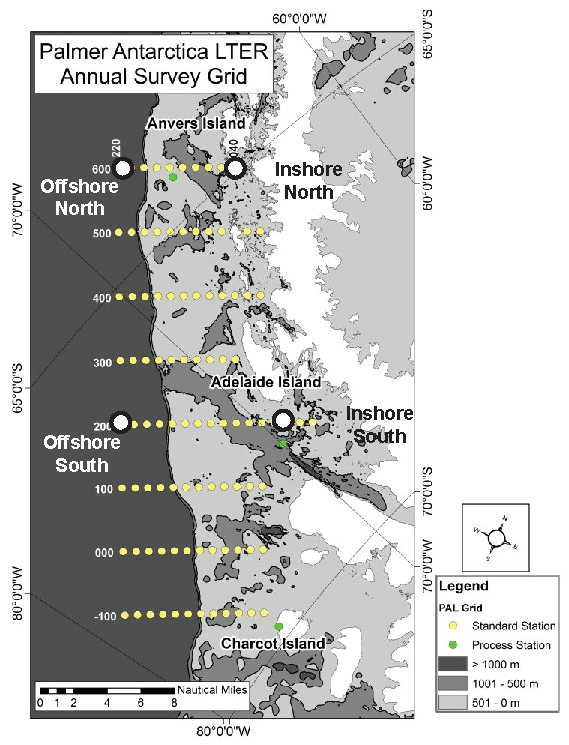
\includegraphics{Chapter_2_MIRADA/Figures/Figure_1_Map} 
	\caption[Map of the Palmer LTER study region.]{Palmer LTER study region along the western Antarctic Peninsula. The white circles indicate the sampling sites.~Land is shown in white, shades of gray indicate depth of water offshore according to legend, and numbers along the sampling grid correspond to LTER designated sampling names.} 
	\label{fig:ltergrid} 
\end{figure}

We sampled and described all three domains of microbial life---Eukarya, Bacteria, and Archaea---through small subunit (SSU) rRNA gene hypervariable amplicon sequencing in order to investigate spatio-temporal variation within domains and the linkages between microbial trophic levels. We found evidence of vertical stratification and temporal variation in community structure corresponding to the seasonal evolution of the upper water column. There were few differences between northern and southern sites. Significant variation between northern and southern assemblages was only evident for microbial eukaryotes and not their bacterial and archaeal counterparts. These results provide core data for comparative study with other aquatic systems, and furnish a baseline against which future changes may be assessed on a range of time and space scales.

\section{Materials and Methods}\label{sc:materials-and-methods}

\subsection{Sample Collection and Processing}\label{ssc:sample-collection-and-processing}

Sampling was conducted on the annual Palmer LTER midsummer research cruise (January -- February 2008). We drew samples from \SI{10}{\m} and \SI{100}{\m} depths from the northern and southern, inshore and offshore corners of the Palmer LTER sampling grid that lies along the western coast of the Antarctic Peninsula (Figure \ref{fig:ltergrid}). We collected duplicate samples using a rosette equipped with 10-liter Niskin bottles and Conductivity, Temperature and Depth (CTD) sensors. To contrast summer and winter water, we also collected an additional Austral winter sample from \SI{10}{\m} depth at the northern, inshore sampling site in August 2008 using a submersible pump with silicone tubing. Environmental data, including nitrate (\ce{NO3}), phosphate (\ce{PO4}), silicate (\ce{SiO4}), particulate nitrogen (P\ce{N}), total nitrogen (T\ce{N}), particulate organic carbon (PO\ce{C}), dissolved organic carbon (DO\ce{C}), chlorophyll \textit{a} (chl \textit{a}), \ce{14C}-primary production, and bacterial abundance and production, were collected through the Palmer Station LTER (\url{http://oceaninformatics.ucsd.edu/datazoo/data/pallter/datasets}). Protocols for these measurements are available in the metadata for each environmental variable. Limited environmental data were available for the winter sample.

We filtered water samples (\SIrange{1}{2}{\L}) through \SI{0.2}{\micro\m} Sterivex\texttrademark~ cartridges (Millipore, Billerica, MA), preserved genomic DNA by flooding the 2-ml filter cartridge reservoir with sucrose lysis buffer (40 mM EDTA, 50 mM \ce{Tris-HCl}, 0.75 M sucrose), and stored the filters at -80\textdegree C until processing. We extracted DNA using a Puregene DNA extraction kit (Qiagen, Valencia, CA) with modifications as described in \citet{amdh09} and stored the DNA at -20\textdegree C until PCR amplification. Bacterial and archaeal V6 16S rRNA and eukaryotic V9 18S rRNA gene hypervariable regions were amplified as described previously \citep{hwmhnbs07, amdh09}, using ``barcoded'' primers which allowed for multiplexed sequencing (see \url{http://vamps.mbl.edu/resources/primers.php} for details). For each sample, we pooled triplicate \SI{50}{\micro\l} PCR reaction products to minimize propagation of PCR errors and purified them using a QIAquick column-based purification kit (Qiagen, Valencia, CA). We sequenced purified amplicons on a 454 Genome Sequencer FLX (Roche, Basel, Switzerland) according to the manufacturer's protocols using the LR70 kit. We trimmed and filtered raw sequence reads as previously described \citep{hhmsw07}. Briefly, 5 bp barcodes were detected and removed, if exact matches to the barcode were not recovered these reads were discarded. Further quality filtering was achieved by requiring exact matches to the proximal and distal primers, removal of any N's in the sequence reads, and removal of all reads less than 50 nucleotides in length. We assigned Operational Taxonomic Units (OTUs) at a 3\% (Bacteria and Archaea) or 6\% (Eukarya) sequence identity clustering level (SLP-PWAL; \citet{hwms10}). We chose a more conservative cut-off for eukaryotic clustering to accommodate microheterogeneities existing in many eukaryotic taxa. In many cases, we were able to achieve genus-level identifications with this cluster width. We also removed all metazoan OTUs from downstream analyses.

\subsection{Alpha and Beta Diversity Estimation}\label{ssc:alpha-and-beta-diversity-estimation}

We determined parametric modeling-based estimates of species richness for Bacteria and Archaea using the CatchAll program \citep{bunge2012estimating} and estimated eukaryotic richness using the non-parametric Chao2 estimator in SPADE \citep{cs10}. For multivariate methods, we employed bacterial and archaeal abundance matrices while eukaryotic abundances were converted to incidence-based (presence/absence) matrices. PC-ORD \citep{p10} was used to conduct a two-way cluster analysis for the archaeal dataset. We generated Morisita-Horn similarity indices for Bacteria and Archaea in EstimateS \citep{c09} and employed Jaccard similarity indices for eukaryotic data in Primer-E (v6, Plymouth, UK). Bray-Curtis and Morisita-Horn similarity indices were generated for resampled bacterial and archaeal data sets. SIMPROF (Primer-E) analyses allowed us to test for significant differences between biological replicates while ANOSIM allowed us to test for differences between samples. We visualized the results using non-metric multidimensional scaling (NMDS) (Primer-E). We performed all calculations using complete abundance matrices, as well as resampled matrices in which the number of sequences reads per sample was made equal through random resampling: 1219 sequences per sample for Bacteria (3218 with replicates pooled), 1005 for Archaea (2502 with replicates pooled), 2370 for Eukarya (4911 with replicates pooled). We only showed resampled data results where resampling deviated from the full dataset result.

\subsection{Unimodal Multivariate Analysis}\label{ssc:unimodal-multivariate-analysis}

We employed CANOCO 4.5 (Microcomputer Power, Ithaca, NY) \citep{Ter-Braak:2002aa} to relate our OTUs to environmental properties. Environmental data were transformed using $ln(x + 0.1)$ and temperature was adjusted to remove negative values by adding 1\textdegree C to each value. Preliminary Detrended Correspondence Analysis yielded gradients close to three so we chose to continue our analyses using the CCA unimodal approach. We employed the automatic forward selection feature in CANOCO to ensure selection of parameters that have low cross-correlation and explain the most variance. The significance of the first CCA axis and all CCA axes combined was tested using Monte Carlo permutation tests with 499 permutations \citep{Ter-Braak:2002aa}.

\subsection{Network Analysis and Data Visualizations}\label{ssc:network-analysis-and-data-visualizations}

We examined co-occurrence patterns across domains using network analysis and significant linear Pearson correlations. For the input matrices we removed all singleton OTUs and only considered OTUs that occurred in at least 50 percent of the samples. We used Cytoscape \citep{smobwr} to visualize the resulting data and only considered significant correlations with an R-value \textgreater{}0.9. We generated bacterial taxonomic bar graphs using Global Alignment Sequence Taxonomy (GAST) \citep{hdhwrs08} and used Qiime v1.4.0 \citep{Caporaso2010-ee} to graphically display the output. The R package routines gplots and heatmap.2 were used to generate the heatmap summary of all microbial eukaryotic OTUs that were encountered with a frequency of greater than 1\% in a given site \citep{t08}. All of our sequence data are MIMARKS-compliant \citep{Yilmaz:2011aa} and have been deposited in the National Center for Biotechnology Information normal and Sequence Read Archives under the accession number SRP041427. Bacterial V6 data were previously deposited under SRP016030 while Eukaryotic V9 were previously deposited under SRP000903. Copies of the MIMARKS table and chapter figures can be accessed at: \url{https://github.com/cmluria/dissertation/Chapter_2_MIRADA}. 

\section{Results}\label{sc:results}

\subsection{Sampling site characteristics}\label{ssc:sampling-site-characteristics}

\afterpage{
\clearpage
\begin{landscape}
\begin{table}
\centering
\caption[Contextual data for sites sampled.]{Contextual data for sites sampled. Differences between depths, inshore and offshore, and north and south comparisons between samples were assessed using student’s t-tests.}
\label{ch1:tab1}
\small
\begin{tabular}{@{}lllllll@{}}
\toprule
Variable                                                     & 10-m Overall & 100-m Overall & 10-m Inshore & 10-m Offshore & 10-m North & 10-m South\\ \midrule
Density                                                      & 27.2**            & 27.4**             & 27.2              & 27.2               & 27.2**          & 27.1**          \\
Salinity                                                     & 33.8**            & 34.2**             & 33.8              & 33.9               & 33.8            & 33.8            \\
Oxygen (µmol/l)                                              & 357*              & 276*               & 366               & 348                & 362             & 352             \\
Temperature (°C)                                             & 0.756             & -0.224             & 0.773             & 0.739              & 0.765           & 0.747           \\
NO3 (µmol/l)                                                 & 18.6*             & 24.8*              & 16.5*             & 20.8*              & 19.5            & 17.8            \\
NO2 (µmol/l)                                                 & 0.38              & 0.28               & 0.25              & 0.5                & 0.35            & 0.4             \\
PON (µmol/l)                                                 & 47.6              & ND                 & 79.9              & 15.2               & 69.2            & 25.9            \\
Total N (µmol/l)                                             & 28.3**            & 36.3**             & 25.1*             & 31.4*              & 29.4            & 27.2            \\
PO4 (µmol/l)                                                 & 1.58***           & 2.10***            & 1.50*             & 1.65*              & 1.6             & 1.55            \\
Si (µmol/l)                                                  & 53.2              & 68.6               & 70.8**            & 35.5**             & 53.2            & 53.2            \\
DOC (µmol/l)                                                 & 45.7              & 43.4               & 46.4              & 45                 & 46.5            & 45.7            \\
POC (µmol/l)                                                 & 210               & ND                 & 349               & 71.8               & 306             & 115             \\
Chlorophyll \emph{a} (µg/l)                                         & 1.71              & 0.147              & 3.21*             & 0.215*             & 2.13            & 1.3             \\
Fluorescence (mg/m$^3$)                                         & 2.3               & 0.189              & 4.1               & 0.506              & 3.14            & 1.47            \\
Bacterial dens. ($10^6$/ml)                                  & 0.227             & 0.225              & 0.242             & 0.212              & 0.189*          & 0.266*          \\
Leucine inc. (pmol/l)                               & 14.6              & ND                 & 22.9              & 6.37               & 18.8            & 10.5            \\ \midrule
                                                             &                   &                    &                   &                    &                 &                 \\
\multicolumn{7}{l}{* $p < 0.1$, ** $p < 0.05$, *** $p < 0.01$}  
\end{tabular}
\end{table}
\end{landscape}
}

The waters in the WAP were consistently cold (<1\textdegree C) and experienced dramatic fluctuations in day length and sea ice cover during the study period. In the austral summer, deep samples (100-m) were more saline and had higher nutrient concentrations (\ce{PO4}, \ce{NO3}, TN, \ce{SiO4}), while surface samples (10-m) contained higher phytoplankton biomass (chl \textit{a}; Table \ref{ch1:tab1}). Within surface samples, we observed differences between inshore and offshore sites, with greater bacterial production and organic substrates (POC and PON) at inshore sites (Table \ref{ch1:tab1}). In general there were not significant environmental differences between the corresponding northern and southern sampling stations (Table \ref{ch1:tab1}).


\subsection{Microbial Community Structure}\label{ssc:microbial-community-structure}

Our three-domain assessment of the microbial communities of the WAP pelagic ecosystem generated \textgreater{}150,000 bacterial, \textgreater{}50,000 archaeal, and \textgreater{}60,000 eukaryotic rRNA amplicon reads from the Palmer LTER study region along the WAP. We selected these sites in order to examine how microbial communities vary with depth, distance from shore, and latitudinal differences in sea ice cover.

\begin{figure}
	[htbp] \centering 
	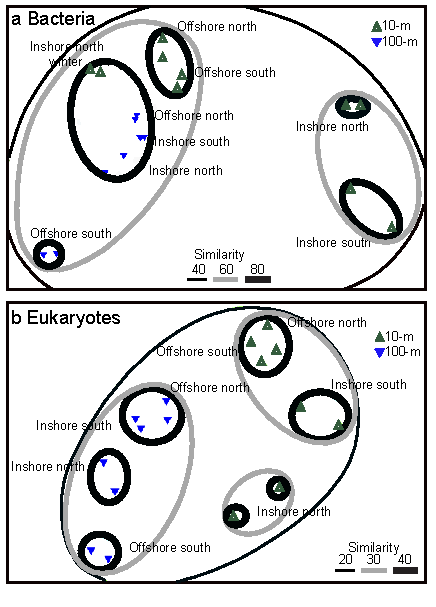
\includegraphics{Chapter_2_MIRADA/Figures/Figure_2_MDS_new_2012_75mm_BW_2013} 
	\caption[Non-metric multidimensional scaling of bacterial Morisita-Horn and eukaryotic Jaccard similarity matrices.]{Non-metric multidimensional scaling of (a) bacterial Morisita-Horn and (b) eukaryotic Jaccard similarity matrices. Bacterial ordination based on samples collected in January and August 2008. Eukaryotic (minus metazoan OTUs) ordination based on samples collected during January 2008 only.} 
	\label{fig:nmds1.1} 
\end{figure}

Bacterial community composition varied significantly by depth (ANOSIM, $p = 0.007$ full, $p = 0.004$ resampled), and slightly among surface samples between inshore and offshore samples (ANOSIM, $p = 0.08$ full, $p = 0.06$ resampled), but showed no significant north-south differences in community structure. NMDS and hierarchical clustering revealed that the inshore surface communities fell into two groups with 60\% similarity, one composed solely of inshore surface samples and one containing all other samples including offshore surface, winter surface and all deep samples, also sharing 60\% similarity (Figure \ref{fig:nmds1.1}). All bacterial samples taken together were 40\% similar to each other. The winter surface sample was more similar to summer deep samples than to any summer surface sample from the same station (Figure \ref{fig:ch1:supp1}). SIMPER analysis showed that 7 OTUs, identified as \textit{Candidatus} Pelagibacter, Oceanospirallales, \textit{Balneatrix}, Flavobacteriaceae, SAR324, \textit{Roseobacter} and Phycisphaeraceae, accounted for over 33\% of the variation between surface and deep communities. Eukaryotes had the greatest degree of variation among samples with some samples having only 20\% similarity. Eukaryotic community composition varied significantly with depth and distance from shore (ANOSIM, $p = 0.001$ and 0.03 respectively for the full dataset; $p= 0.001$ and 0.027 for the resampled dataset), but as with bacterial communities failed to exhibit large differences in beta diversity (between sample diversity) between the north and south stations. Individual eukaryotic OTUs were unable to explain more than 0.5\% of this variation (SIMPER). We detected little variation among archaeal communities (summer 100-m and winter surface) due in part to our inability to detect archaea in surface summer samples and there were few differences in the structure of corresponding northern and southern communities (e.g., northern vs.~southern inshore samples) (Figure \ref{fig:cca1.1}). We did observe significantly higher eukaryotic alpha diversity (species richness) at the northern inshore site (Figure \ref{fig:richness1}) and differences in the relative recoveries of individual eukaryotic OTUs (Figure \ref{fig:ch1:supp2}).

\begin{figure}[htbp] 
\centering 
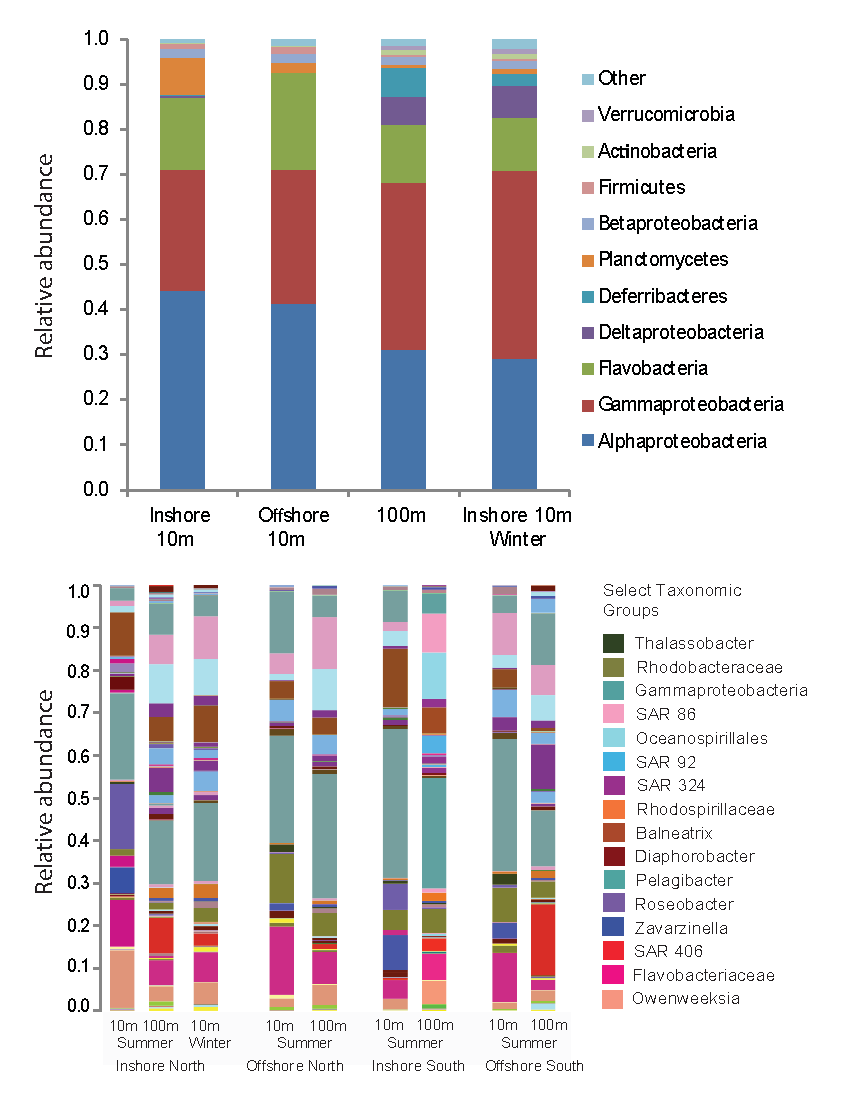
\includegraphics[width=1.0\textwidth]{Chapter_2_MIRADA/Figures/Supplemental_1_Qiime_taxonomic_summary} 
\caption[Relative abundance of most common bacterial taxa from different sets of sites.]{Relative abundance of most common bacterial taxa from (a) coarser taxonomic resolution for inshore and offshore 10 m (north and south pooled), 100 m (north and south inshore and offshore pooled), and winter inshore surface (north only) samples. (b) More fine scaled taxonomic resolution bar graphs for summer vs.~winter, inshore vs.~offshore, and North vs.~South.} 
\label{fig:ch1:supp1} 
\end{figure}


\begin{figure}
	[htbp] \centering 
	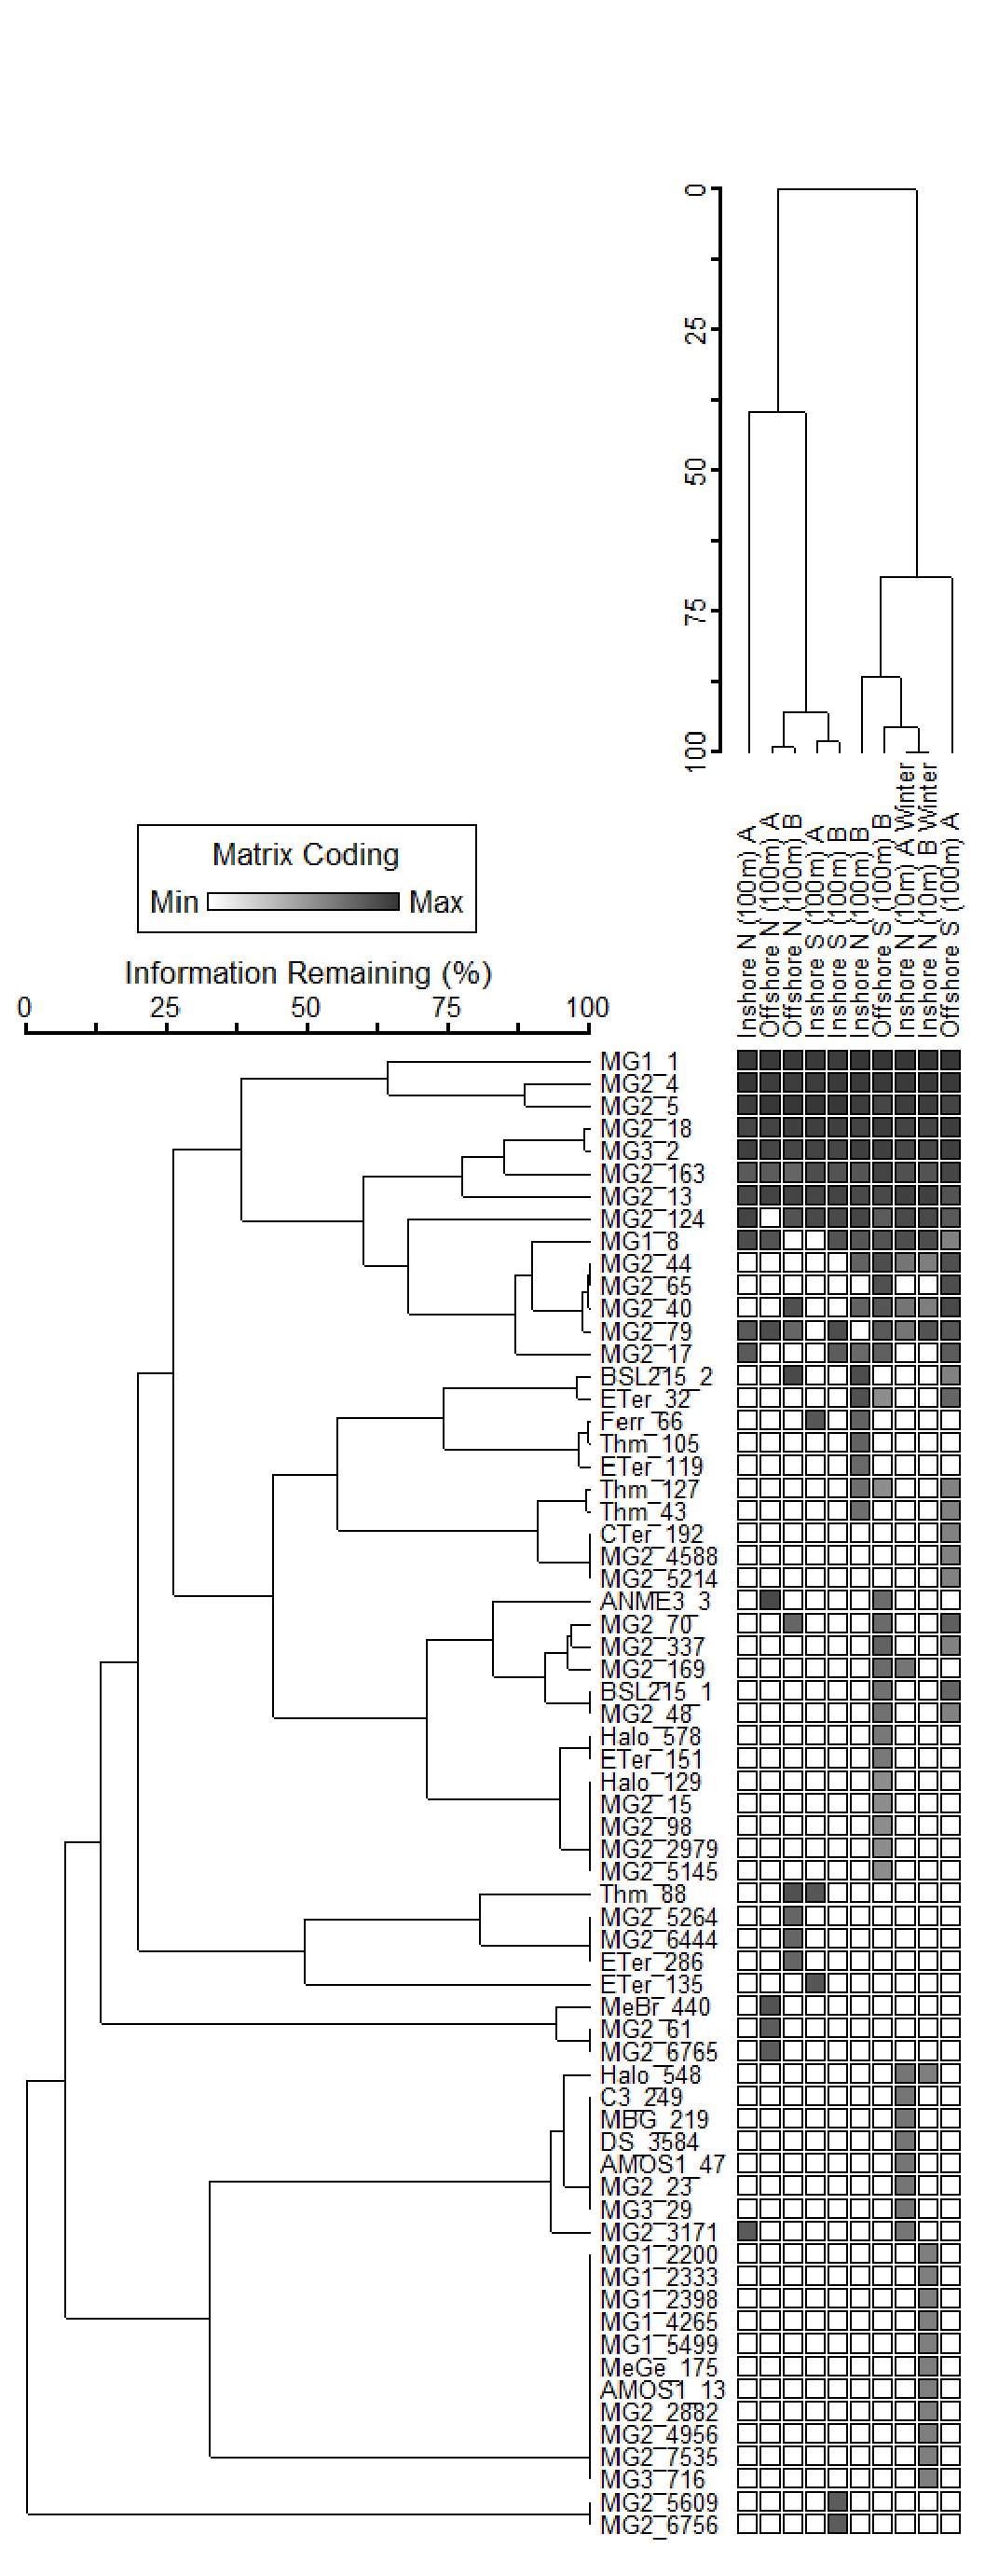
\includegraphics[width=0.5
	\textwidth]{Chapter_2_MIRADA/Figures/Figure_4_PAL_Av6_2way_notrans_Relmax_SOR_aveneigh} 
	\caption[Archaeal two-way cluster analysis.]{Archaeal two-way cluster analysis. Samples were collected from 100-m depth in January 2008 and from the surface in August 2008 (winter). Abbreviations are as follows: MG1 (Marine Group I Crenarchaeota; MG2 Marine Group II Euryarchaeaota; MG3 Marine Group III Euryarchaeota; remaining are miscellaneous Euryarchaeota groups). The matrix coding denotes the relative abundance within the matrix for a given OTU.} 
	\label{fig:cca1.1} 
\end{figure}

\begin{figure}
	[htbp] \centering 
	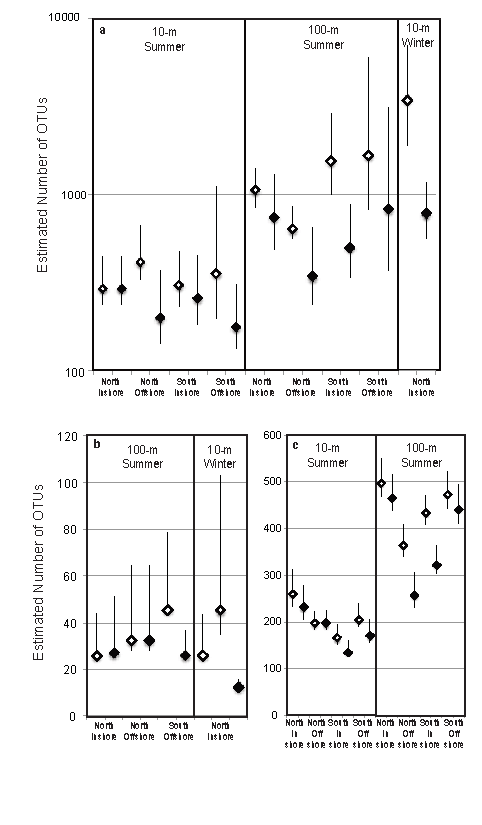
\includegraphics[width=0.7
	\textwidth]{Chapter_2_MIRADA/Figures/Figure_6_PAL_alpha_comp_75mm} 
	\caption[Estimated OTU richness for Bacteria, Archaea, and Eukarya at different sites.]{Species richness estimates of: (a) bacterial, (b) archaeal and (c) eukaryotic OTUs with Bonferroni-corrected 95\% confidence intervals for all samples across a given domain. Filled diamonds are for resampled data. For each of the bacterial samples two replicates were pooled. Eukaryotic diversity estimation required the two replicate samples to calculate a single incidence-based richness estimate for a given pair of samples. For archaeal estimates, south offshore 100-m and winter north inshore replicates are shown individually, north and south offshore 100-m replicates were pooled, and north offshore 100-m estimates were not done. Bacterial and archaeal estimates were calculated using CatchAll while eukaryotic estimates were calculated using Chao2 as implemented in SPADE.} \label{fig:richness1} 
\end{figure}

\begin{figure}[htbp] 
\centering 
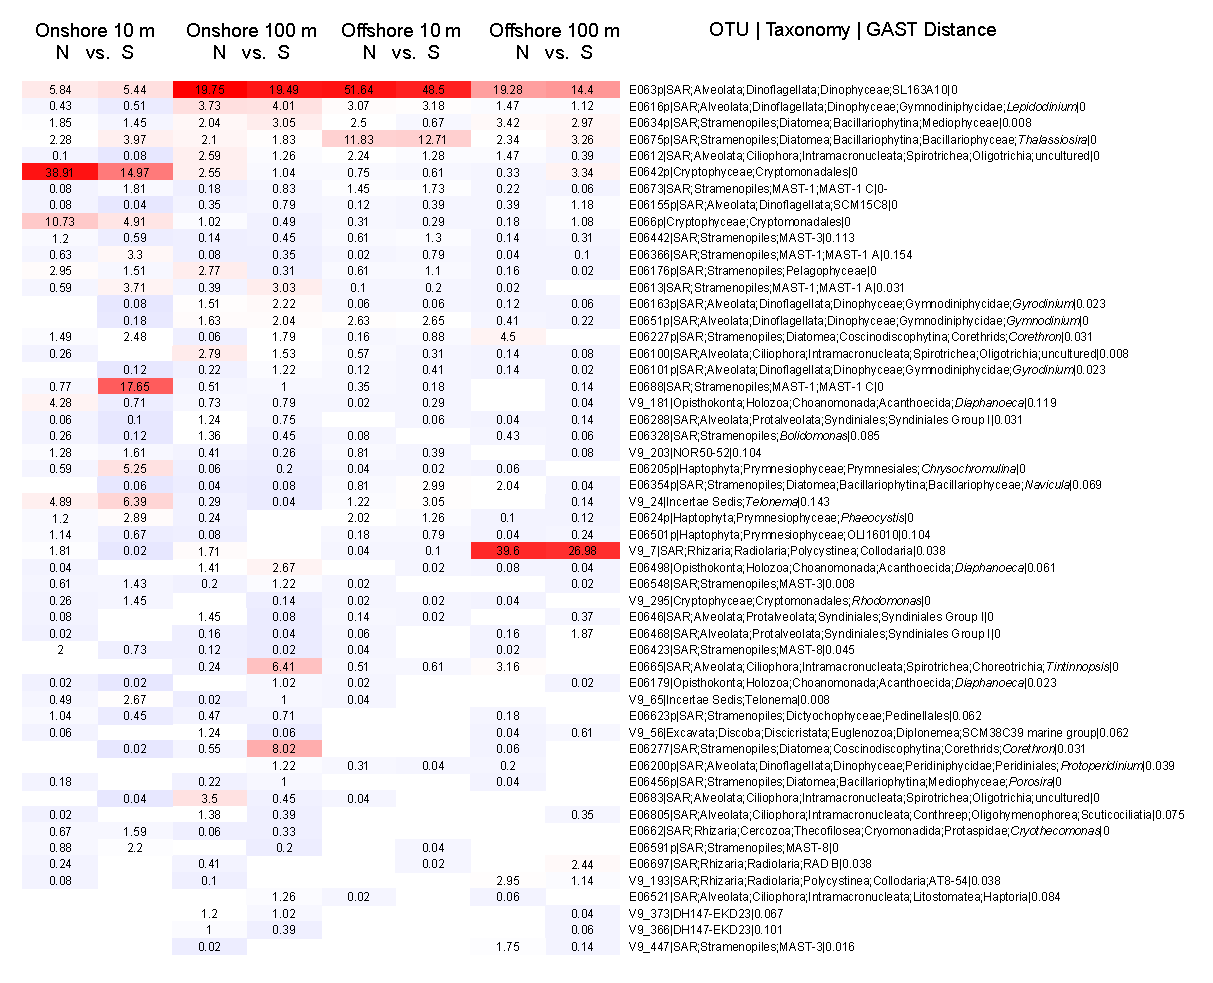
\includegraphics[width=\textwidth]{Chapter_2_MIRADA/Figures/Supplemental_2_euk_random_Rplot_4ms} 
\caption[Heatmap of eukaryotic OTUs.]{Heatmap of eukaryotic OTUs recovered at a frequency of more than 1\% at a given station. Hot colors indicate higher percentages while cooler colors indicate lower percentages, with actual values superimposed over colors. Data shown are normalized by randomly resampling data to the lowest sampling effort. The depth of taxonomic resolution available in the V9 region varied by taxon and is displayed to the right along with Global Alignment for Sequence Taxonomy \citep{hdhwrs08} distance values to the nearest relative in GenBank.} 
\label{fig:ch1:supp2} 
\end{figure}

\begin{figure}
	[htbp] \centering 
	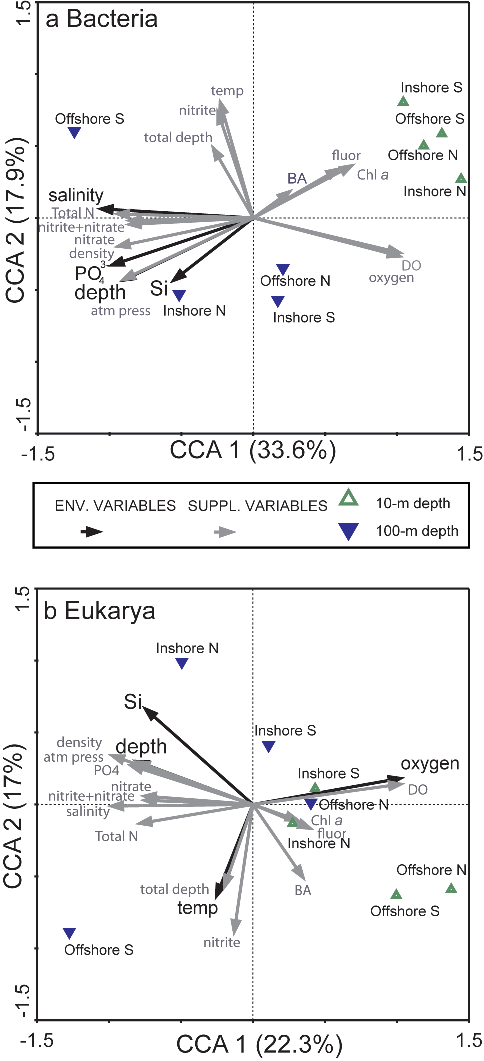
\includegraphics{Chapter_2_MIRADA/Figures/Figure_3_CCA} 
	\caption[Canonical correspondence analysis based on summer bacterial and eukaryotic OTU libraries.]{Canonical correspondence analysis based on (a) bacterial and (b) eukaryotic OTU libraries from water samples collected in January 2008. Explanatory variables (black arrows) and supplementary variables (grey lines) are shown.} 
	\label{fig:cca1.2} 
\end{figure}

We conducted further analyses to identify the linkages between community composition and environmental conditions. We were especially interested in co-occurrence patterns between bacteria and photosynthetic eukaryotes. CCA biplots summarized the relationships between environmental variables and bacteria and eukaryotes (Figure \ref{fig:cca1.2}). The underlying environmental variables determining community structure differed between bacterial and eukaryotic domains. For bacteria, CCA axis 1 was most closely correlated with salinity while CCA axis 2 was most closely correlated with silicate. The first CCA axis explained 33.6\% of the variance in the dataset and the first two axes combined explained 51.5\%. In addition to salinity and silicate, depth and phosphate were also significant explanatory variables shaping bacterial community structure. More so than NMDS, the bacterial CCA analysis showed a marked separation between shallow and deep samples along the vertical salinity gradient. As with NMDS, no obvious north-south separation between samples was evident in our biplots.


Eukaryotic CCA analysis showed a less marked difference between community structures at 100-m than for bacterial communities. The first CCA axis was defined by oxygen and the second by temperature and explained 22.3\% (Axis 1) and 39.3\% (Axes 1 \& 2) of the variation in the dataset respectively. The offshore south 100-m sample in particular was most positively correlated with higher temperature as was seen in the bacterial community analyses.

Due to the limited number of archaeal samples relative to environmental parameters available, we chose to conduct a two-way cluster analysis to explore the relationship between samples and OTU groups (Figure \ref{fig:cca1.1}) instead of conducting a CCA. The resulting two-way cluster diagram shows shared OTU groupings among different samples. Unlike bacterial assemblages, winter inshore 10-m archaeal assemblages clustered most closely with offshore summer southern communities. As with both bacterial and eukaryotic samples, no north-south contrast was revealed in our archaeal analyses. Network analyses using significant Pearson correlations identified positive inter-domain (bacterial-eukaryotic) associations between for example, photosynthetic and heterotrophic community members such as diatoms and Rhodobacteraceae, as well as diatom-SAR11 associations \ref{fig:cooccur1}. Our network analyses also revealed intra-domain (eukaryotic-eukaryotic) correlations, possibly symbiotic or parasitic affiliations (Radiolarian-like-protist and dinoflagellate (alveolate) associations), or perhaps just co-occurring protistan taxa shaped by common environmental constraints.

%
\begin{figure}[htbp] \centering 
	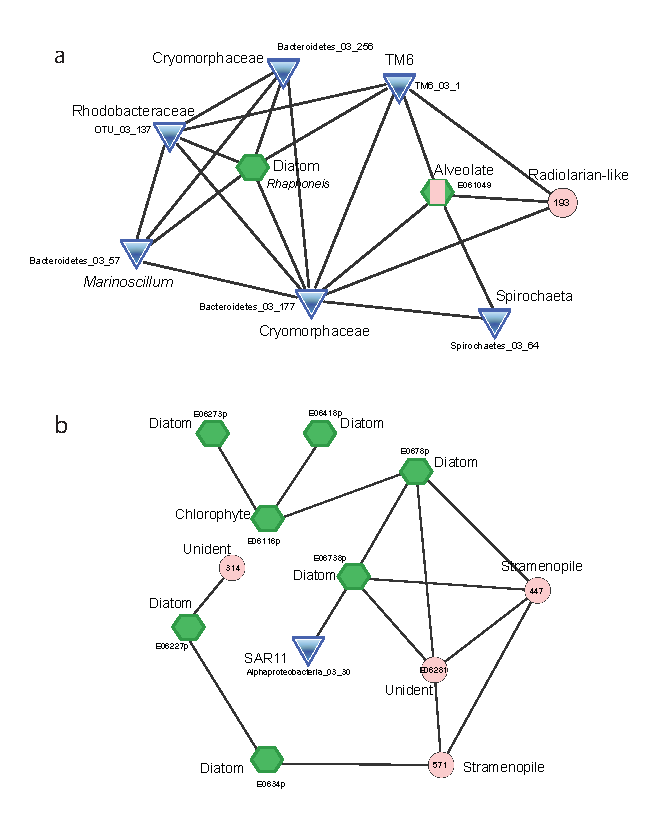
\includegraphics[width=0.9\textwidth]{Chapter_2_MIRADA/Figures/Figure_5_PAL_Ev9Bv6_pooled_50_plusminus90_corr_networkMOD2} 
	\caption[Co-occurrence analysis of combined bacterial and eukaryotic matrices.]{Co-occurrence network analysis of combined bacterial and eukaryotic matrices. Bacteria are indicated by triangles. Lines represent significant Pearson correlations (R>0.9). Pink circles represent microbial eukaryotes that are most likely heterotrophic. Green hexagons represent phototrophs. The pink and green hexagon represents an alveolate of unknown trophic status. (a) A network highlighting Alveolate-Radiolarian interactions, (b) a network focusing on SAR11 and an unknown diatom interaction.} 
	\label{fig:cooccur1} 
\end{figure}

\subsection{Richness and community composition}\label{ssc:richness-and-community-composition}

We detected the highest richness within the bacterial domain (Table \ref{ch1:tab2}, Figure \ref{fig:richness1}a). We observed 234 bacterial OTUs on average with an estimated richness of 520. As with community composition, bacterial richness varied by depth, with 100-m samples having greater observed and estimated diversity (Table \ref{ch1:tab2}, Figure \ref{fig:richness1}a). The winter sample had almost twice the estimated richness (2125) of any summer sample. Over half (51\%) of sequences were classified to the genus level, while an additional 32\% of sequences were identified to the family level. The majority (75 $\pm$ 2\%) of sequences were identified as Proteobacteria, primarily in the Alpha- (36 $\pm$ 3\%) and Gamma- (33 $\pm$ 2\%) subgroups (Figure \ref{fig:ch1:supp1}). Alphaproteobacteria, especially Rhodobacterales, were more important in surface samples, accounting for 43 $\pm$ 2\% of sequences compared to 30 $\pm$ 4\% at 100-m. Inshore surface samples were distinguished by high prevalence of \textit{Roseobacter} (15\% in the north and 6\% in the south). \textit{Candidatus} Pelagibacter (SAR11) was more consistent across surface samples, accounting for 23 $\pm$ 2\% of all sequences. Gammaproteobacteria, primarily SAR86, SAR92, Oceanospirillales, \textit{Balneatrix} and a number of unclassified OTUs, had greater relative abundance in deep samples, accounting for 36 $\pm$ 1\% of sequences. Deltaproteobacteria, especially Desulfobacterales, Nitrospinaceae, and SAR324, were more common at 100-m depth, accounting for 7 $\pm$ 3\% of sequences in deep samples but \textless{}1\% in surface samples. The bulk of the remaining sequences consisted of Flavobacteria, Planctomycetes, and Deferribacteres. Flavobacteria were most abundant in the northern inshore site (28\%). Planctomycetes, especially \textit{Zarvarzinella}, were common at both northern and southern inshore sites (8 $\pm$ 1\%). Deferribacteres were mostly found at 100-m depth (7 $\pm$ 3\%).

\afterpage{
\begin{landscape}
\begin{table}[]
\scriptsize
\centering
\caption[Observed and estimated richness for Bacteria, Archaea, and Eukarya]{Observed and estimated richness for Palmer Station LTER samples using 97\% similarity values for Bacteria and Archaea and 94\% similarity values for Eukarya. Samples for Bacteria and Archaea were pooled unless indicated with a replicate designation after the sample number (e.g. 9.1). Both replicates were used to calculate the eukaryotic diversity estimates. }
\label{ch1:tab2}
\begin{tabular}{@{}lclllllllllll@{}}
    &                                  &           &       & \multicolumn{3}{c}{ARCHAEA}          & \multicolumn{3}{c}{BACTERIA}         & \multicolumn{3}{c}{EUKARYA**}        \\ \midrule
ID  & \multicolumn{1}{l}{Location}     & Depth (m) & Month & No. of Reads & Obs. OTUs & Est. OTUs & No. of Reads & Obs. OTUs & Est. OTUs & No. of Reads & Obs. OTUs & Est. OTUs \\ \midrule
1   & \multirow{2}{*}{Inshore, north}  & 10        & Jan   & -            & -         & -         & 3218         & 126       & 289.4     & 6369         & 211       & 259       \\
1*  &                                  & 10        & Jan   & -            & -         & -         & 3218         & 126       & 289.4     & 4911         & 188       & 229.3     \\
2   & \multirow{2}{*}{Inshore, north}  & 100       & Jan   & 4295         & 21        & 25.7      & 11454        & 513       & 1050.4    & 5568         & 430       & 498       \\
2*  &                                  & 100       & Jan   & 2502         & 20        & 27        & 3218         & 303       & 735.4     & 4911         & 405       & 466.7     \\
3   & \multirow{2}{*}{Offshore, north} & 10        & Jan   & -            & -         & -         & 17676        & 195       & 415       & 4911         & 177       & 194.1     \\
3*  &                                  & 10        & Jan   & -            & -         & -         & 3218         & 103       & 198.8     & 4911         & 176       & 194.5     \\
4   & \multirow{2}{*}{Offshore, north} & 100       & Jan   & 2502         & 21        & 32.3      & 29555        & 350       & 630.3     & 11775        & 313       & 363.5     \\
4*  &                                  & 100       & Jan   & 2502         & 21        & 32.3      & 3218         & 155       & 340.9     & 4911         & 211       & 255.2     \\
5   & \multirow{2}{*}{Offshore, south} & 10        & Jan   & -            & -         & -         & 11845        & 143       & 353.5     & 9078         & 180       & 204.9     \\
5*  &                                  & 10        & Jan   & -            & -         & -         & 3218         & 93        & 176.7     & 4911         & 147       & 169.9     \\
6   & \multirow{2}{*}{Offshore, south} & 100       & Jan   & 9724         & 34        & 45.4      & 21306        & 585       & 1678.4    & 5996         & 407       & 472.6     \\
6*  &                                  & 100       & Jan   & 2502         & 24        & 25.9      & 3218         & 260       & 819.4     & 4911         & 375       & 440.8     \\
7   & \multirow{2}{*}{Inshore, south}  & 10        & Jan   & -            & -         & -         & 4869         & 146       & 303.4     & 7623         & 145       & 162.8     \\
7*  &                                  & 10        & Jan   & -            & -         & -         & 3218         & 120       & 256.8     & 4911         & 125       & 136.4     \\
8   & \multirow{2}{*}{Inshore, south}  & 100       & Jan   & -            & -         & -         & 37524        & 546       & 1551.5    & 11500        & 387       & 431.4     \\
8*  &                                  & 100       & Jan   & -            & -         & -         & 3218         & 206       & 493.9     & 4911         & 285       & 323.3     \\
9.1 & \multirow{2}{*}{Inshore, north}  & 10        & July  & 11941        & 21        & 25.9      & -            & -         & -         & -            & -         & -         \\
9.2 &                                  & 10        & July  & 16026        & 24        & 45.3      & -            & -         & -         & -            & -         & -         \\
9   & Inshore, north                   & 10        & July  & -            & -         & -         & 18410        & 645       & 3474.8    & -            & -         & -         \\
9*  &                                  & 10        & July  & 2502         & 12        & 12.2      & 3218         & 273       & 775.2     & -            & -         & -         \\ \midrule
    &                                  &           &       &              &           &           &              &           &           &              &           &           \\
\multicolumn{3}{l}{*Randomly resampled data.}      &       &              &           &           &              &           &           &              &           &           \\
\multicolumn{3}{l}{**Metazoan reads removed.}      &       &              &           &           &              &           &           &              &           &          
\end{tabular}
\end{table}
\end{landscape}
}


Eukaryotic rRNA gene V9 hypervariable-region sequencing yielded an overall average of 260 observed and 300 estimated OTUs. We did not sequence eukaryotic winter samples so we are unable to contrast seasonal richness patterns in eukaryotes; however, we can say that overall, deeper samples were significantly richer than surface samples. More importantly, we detected increased eukaryotic richness in surface (10 m) and deep (100 m) inshore northern stations as compared to southern ones, but offshore northern and southern stations revealed either no difference or increased richness at depth in the south. Surprisingly, dinoflagellate-related OTUs that constituted the largest eukaryotic OTU class type in our dataset (Figure \ref{fig:ch1:supp2}) did not show depth patterns that were consistent with our expectation that photoautotrophs dominate the euphotic zone and heterotrophs deeper waters, nor did high-performance liquid chromatography-derived pigment data suggest that a disproportionate fraction of the phototrophic community was composed of dinoflagellates. Cryptophytes and diatoms, also among the numerically dominant phototrophs, did not show surface and depth contrasts that might be anticipated of strict phototrophy. This is in contrast to groups like haptophytes which showed increased amplicon read numbers at 10-m vs.~100-m depths. Within 10-m samples, we observed greater relative abundances of cryptophytes at inshore sites while offshore sites were dominated by dinoflagellates and diatoms (Figure \ref{fig:ch1:supp2}). Archaea had the lowest richness of the three domains, with an average of 22 observed and 33 estimated OTUs (Table \ref{ch1:tab2}). Marine Group I Crenarchaeota (MG1: Thaumarchaeota) and Marine Groups II and III (MG2, MG3) Euryarchaeota dominated our samples accompanied by a number of less abundant Thermoplasmatales, Halobacteriales, and Methanosarcinales. MG3 was significantly more abundant ($p<0.05$) in our summer northern inshore and southern offshore samples (8\% relative abundance vs.~0.5\% for all other samples). The winter assemblage differed from summer assemblages with a higher abundance of Thaumarchaeota (80\%) and a lower abundance of MG2 (19\%).



\section{Discussion}\label{sc:discussion}

\subsection{Seasonal, vertical and spatial variation in phytoplankton-heterotroph coupling}\label{ssc:seasonal}

We observed significant differences in microbial community structure (and apparent differences in archaeal abundance) based on depth (10-m and 100-m) (bacteria and eukaryotes), proximity to shore (eukaryotes) and between winter and summer seasons (bacteria and archaea). Depth-based differences were consistent with previous reports of strong vertical stratification in community composition in other environments \citep{dk05,bpbsblfd09}. Results from CCA showed that bacterial and eukaryotic community composition correlated with salinity and silicate for bacteria and temperature and oxygen for eukaryotes: all factors that are influenced by water column vertical stratification. In this context, the similarity between our 10-m surface winter sample and our 100-m summer samples is not surprising. This similarity reflects the origin of the summertime, minimally-modified remnant ``Winter Water'' below the seasonal thermocline \citep{msisv08,dsvse12}. During the Antarctic winter, the water column is divided into two main water masses: warm, nutrient-rich Circumpolar Deep Water (CDW) overlaid by cold, relatively fresh Antarctic Surface Water (AASW) \citep{cmmkpbs07,msisv08}. The AASW results from convective mixing and cooling in winter and can extend to several hundred meters in depth. In the spring, increasing surface temperatures and meltwater from sea ice and glaciers result in water column stratification and the isolation of a deep remnant of the cold, now relatively saline AASW. This cold remnant with a core at about 100 meters is traditionally known as Winter Water (WW) \citep{m34}. Previous findings suggested that WW 100-m communities in summer and winter surface microbial communities might share some features, including more abundant archaea \citep{mtmwjd98,Church2003-oj}. Furthermore, in a comparison of clone libraries generated from winter and summer surface water samples, \citet{grwddecm12} found increased abundance of genes related to chemolithoautotrophy, typically found in deeper marine habitats, during the Antarctic winter. Our results demonstrate that seasonal patterns in WAP water column structure are reflected in bacterial and archaeal community composition.

Several lines of evidence suggest that the mechanism driving the observed succession of microbial community structure from winter to summer is enrichment by organic matter generated by photoautotrophs. Order of magnitude increases in bacterial production rates \citep{dsvse12} must be accompanied by increased resources. The summer bacterial community is characterized by many sequences indicating heterotrophic capabilities \citep{grwddecm12}. Microautoradiography-FISH determinations showed that the most abundant OTUs utilized amino acids and dissolved proteins \citep{straza2010abundance}. A summer bacterial community from the WAP demonstrated reduced diversity in response to experimental glucose enrichment, consistent with our field observations \citep{dmegm11}. In contrast, a summertime sample from the Mediterranean Sea grown over five generations (15 days) in continuous culture in the presence of a complex substrate derived from a phytoplankton culture exhibited increased diversity relative to an unamended control \citep{lckbo13}. The samples and experimental conditions differed between these experiments, preventing simple conclusions about relationships between organic enrichment and diversity.

In the present study, we did not find a significant correlation between phytoplankton biomass and bacterial community composition within summer 10-m samples, although CCA analyses showed silicate to be a significant factor influencing bacterial community structure. The LTER study grid encompasses an inshore-offshore gradient with average (1993-2013) phytoplankton biomass ranging from 4 mg chl \textit{a} m$^{-3}$ on the coast to 0.3 mg chl \textit{a} m$^{-3}$ over the continental slope (\url{http://pal.lternet.edu/data};  \citealt{gvf05,sdv96,sbbs98,sbv98}). We observed high phytoplankton biomass (chl \textit{a}) at the inshore stations in the present study. Despite marked differences in chlorophyll and eukaryotic community composition, unlike eukaryotic communities, bacterial community composition between inshore and offshore sites was only significantly different at the 90\%, but not at the 95\% confidence level based on our ANOSIM analyses. While eukaryotic communities were much less similar to each other overall than bacterial communities, caution should be applied in interpreting absolute magnitudes of the similarity values between abundance-based data (bacteria) and presence/absence (eukaryotes) data. We suggest that none of the surface bacterial communities were carbon-limited in summer but that the relative differences in phytoplankton biomass between sites may have in some way influenced bacterial community composition.

\subsection{Community composition across three domains}\label{ssc:community}

Most studies of bacterial diversity in Antarctic waters have used culture-dependent or community fingerprinting techniques. For example, significant inter-seasonal variation in bacterial community composition was found using DGGE \citep{mpmtbwd98,mg07}. A few studies have used clone libraries to investigate bacterial diversity, finding high diversity within the Gammaproteobacteria and Cytophaga-Flavobacteria-Bacteroidetes (CFB) divisions \citep{ggdsad06,Piquet2011-ot}. More recently, studies have adopted next-generation sequencing approaches to contrast sub-Antarctic and Antarctic bacterial community richness, structure and biogeography \citep{Ghiglione2012-qm, wlwdbhamrrc13, wvrlc13}.

Alphaproteobacteria, Gammaproteobacteria, and Bacteroidetes dominated the bacterial communities we sampled (c.f. \citet{ggdsad06, pcrbslth07, Piquet2011-ot,Ghiglione2012-qm, wlwdbhamrrc13, wvrlc13}. We identified abundant amplicons from several ``ubiquitous'' clusters such as SAR11, SAR86, and SAR324 \citep{pph05}, but also noted the absence of cyanobacteria such as \textit{Prochlorococcus} and \textit{Synechococcus} that are typically absent or rare in bacterial communities in the Antarctic Zone \citep{wlwdbhamrrc13,wywabdlc13}. In addition to the ubiquitous and dominant SAR11, \textit{Roseobacter} was another significant alphaproteobacterium that was likely associating with phytoplankton at shallow depths \citep{Ghiglione2012-qm,wlwdbhamrrc13,wywabdlc13}.

Despite a growing body of knowledge, linking microbial community composition to function remains a significant challenge. However, the contrasts we observed among the abundances of different taxa are suggestive of coupling between primary productivity and bacterial/archaeal presence and community composition. Although overall community composition did not vary significantly among surface samples, a few clades displayed marked differences in relative abundance between sites, indicating different ecological niches at different sampling locations. For example, Planctomycetes, especially \textit{Zarvarzinella}, were more abundant at near-shore sites where algal biomass was highest, in contrast with previous studies wherein Planctomycetes were detected in low abundance in the Southern Ocean \citep{wywabdlc13}. Culture-dependent and -independent techniques have shown that the CFB division is particularly prominent in situations with high DOC availability, e.g. in sea ice \citep{bkjwah03} or during phytoplankton blooms \citep{Glockner1999-yc,Abell2005-vh} perhaps due to superior competitive exploitation of algal-derived carbon \citep{pfgwwa11}. Positive associations between diatoms and Rhodobacteraceae, Cryomorphaceae, and SAR11 respectively in our study also suggest coupling between heterotrophs and photoautotrophs. The significantly increased relative abundance of some proteobacterial clusters (e.g.~Desulfobacterales, Nitrospinaceae, SAR324) in our 100-m samples could indicate that chemolithotrophy is relatively important deeper in the water column \citep{grwddecm12} in the summer. This is consistent with a previous report of Desulfobacterales in winter samples in the Antarctic Peninsula \citep{Ghiglione2012-qm} and SAR324's inferred role in chemautotrophy in the cold, dark ocean \citep{smpswlrpmgsdhs11}. Similarly, archaeal abundance was apparently very low in summer surface waters. These bacterial and archaeal distribution patterns may reflect inability of chemolithotrophs to compete successfully under summer conditions.

A notable aspect of our study was our use of amplicon pyrosequencing to assess the diversity of all three microbial domains, including eukaryotes. Our study detected similar magnitude and trends in increased bacterial richness in winter versus summer as reported previously \citep{Ghiglione2012-qm}, but also added insights into archaeal and eukaryotic richness with depth and location relative to the shoreline. Namely, archaea showed opposite trends to bacteria with decreased richness in our resampled datasets in the winter versus summer with overall numbers of OTUs an order of magnitude less than bacteria and eukaryotes. Like bacteria, eukaryotes also displayed increased richness at depth while archaeal richness at different depths was difficult to ascertain given our inability to detect archaea in summer surface samples.

Previous studies of WAP eukaryotic diversity have relied primarily on pigment data and microscopy \citep{rvz02, rjbf02, gvfsrq03, gvkf03, acccg10} or only considered richness \citep{amdh09}. Large diatoms and cryptomonads generally account for the bulk of phytoplankton biomass, while unidentified photosynthetic flagellates are numerically dominant \citep{vhh93, rjbf02, gvkf03, acccg10}. \citet{gvkf03} observed strong inshore-to-offshore gradients in biomass and community composition and attributed differences between northern and southern inshore blooms (cryptomonads in the north versus diatoms in the south) to differential timing of sea ice retreat. Diatom assemblages are highly variable from year to year \citep{acccg10}, although several genera including \textit{Corethron}, \textit{Chaetoceros}, \textit{Fragilariopsis}, \textit{Odontella}, and \textit{Nitzschia} are common \citep{gvfsrq03,acccg10}, and often co-occur with \textit{Phaeocystis antarctica} \citep{rjbf02, gvkf03}. Cryptophytes were more prevalent in the northern surface waters, but dinoflagellates were the most abundant OTU in our study. The prevalence of dinoflagellates was not consistent with our pigment data or microscopic observations. One likely explanation for over-representation of dinoflagellate-related OTUs may be that dinoflagellates are known to possess many copies of their rRNA genes (\textgreater{}12,000 for dinoflagellates such as \textit{Akashiwo sanguinea}; \citealt{zmnmv05}), while picoeukaryotes may have four orders of magnitude fewer. Another more speculative explanation is that perhaps the dinoflagellate signals detected in large quantities in our study are the result of these cells engaging in kleptoplasty (chloroplast theft from other phototrophs) \citep{gmdc07} allowing them to serve as mixotrophs as needed. This may also help explain why we failed to see dinoflagellate-specific pigment signatures in our HPLC data. Another possible explanation is that the detected dinoflagellate signal derives from heterotrophic and not phototrophic dinoflagellates. Results of our network analyses pointed to Group I alveolates known to include parasitic and therefore heterotrophic clades as possible contributors to eukaryotic niche diversity as a whole. Furthermore, diatom and cryptophyte abundance did not vary significantly with depth, suggesting possible alternative survival strategies such as mixotrophy or heterotrophy \citep{bacccgps00,tsrg06} or possible persistence of environmental DNA \citep{cvcl12,cvl12}.

\subsection{Microbial Diversity, Resilience, and Climate Change}\label{microbial-diversity-resilience-and-climate-change}

\citet{cltcl11} conducted a similar, 3-domain pyrosequencing study in the Amundsen Gulf, Canadian Arctic over the 2003-2010 period of rapid warming and sea ice loss. They observed significant changes in community composition within the bacterial, archaeal and eukaryotic domains over time, and reductions in overall bacterial diversity when samples were pooled into pre- and post-2007 groups. The Palmer LTER study region encompasses a strong climatic gradient running roughly north to south along the Antarctic Peninsula \citep{msisv08,smsi08}. Changes have been more dramatic in the northern part of the region, with greater atmospheric and ocean warming \citep{mk05} and larger reductions in sea ice cover. In response the region has experienced reductions in the populations of ice-dependent species such as Adèlie penguins \citep{dcddghmmmms12}, Antarctic krill \citep{aspr04} and large-celled phytoplankton \citep{mddfmss09} over the past few decades. Thus the WAP presents north and south regions at different stages of climate change, sea ice reduction and ecosystem transformation. It is intriguing that despite well-documented latitudinal trends in phytoplankton and higher trophic levels, we only observed significant differences in microbial richness among eukaryotic microbes and not their bacterial and archaeal counterparts. These differences in eukaryotic richness were not consistent between inshore and offshore sites so we assume that they are not merely the effect of diversity increases due to environmental DNA from surface waters. Beta-diversity patterns between northern and southern stations were less obvious except perhaps for northern inshore eukaryotic communities. These observations relate to ongoing questions about microbial biogeography and community resilience.

The similarity observed between northern and southern assemblages may reflect the timing of sampling. We found that the oceanographic conditions at our sampling sites were quite similar at this time (Table \ref{ch1:tab1}). Many WAP latitudinal trends (i.e.~temperature and sea ice duration and extent) are most apparent during autumn, winter, and spring \citep{dcddghmmmms12}. Properties such as sea ice extent or primary production may or may not reflect gradients or longer-term trends in any single year.

Microbial communities can be similar at kilometer distances but dissimilar tens to hundreds of km apart, supporting the idea of coherent community patches in the open sea \citep{hscf06,mncawa12}. Surface currents in the WAP are \textasciitilde{} \SIrange{0.1}{1}{\meter \per\second} \citep{sa09}, giving an advective timescale between the northern and southern stations of 5-10 days. Bacterial assemblages should have ample time for turnover during transit, so latitudinal similarity over this distance due simply to physical mixing is unlikely \citep{wvrlc13}.

Microbial community resilience may also contribute to the observed lack of variation between northern and southern sites overall. Microbial community composition can be sensitive to disturbances in temperature and carbon enrichment among other factors \citep{am08}. However, fast growth rates, metabolic flexibility, and rapid evolution could increase the stability of microbial community composition and facilitate return to a pre-disturbance state. Microbial communities might vary between the north and south during the winter and spring when greater environmental differences are observed, but then quickly reach a common summer community composition. In contrast, larger, longer-lived organisms integrate the effects of change over years (krill) to decades (penguins, seals).

\section{Conclusions}\label{conclusions}

Analysis of microbial eukaryotic, bacterial and archaeal communities from four sites separated by 200 (cross-shelf) and 400 km (alongshelf) along the WAP revealed relatively low spatial variability in microbial community composition. Community composition responded more to the environmental variability represented by 10-m and 100-m depths than to more subtle differences in production and climate forcing between different sites. Northern versus southern patterns in richness were only represented in inshore microbial eukaryotic communities. Furthermore, we found that bacterial and archaeal assemblages in 100-m summer samples were similar to winter surface (10-m) communities reflecting established seasonal patterns in water column stratification and turnover. While we can begin to speculate on relative differences in community function based on SSU rRNA gene amplicon sequencing, further efforts are needed to examine the abundance and expression of functional genes in order to find the connections between microbial communities and ecosystem function in this fragile and rapidly changing region.


\chapter{Seasonal succession of free-living bacterial communities in coastal waters of the Western Antarctic Peninsula}\label{ch:swi}

\chapterdisclaimer{This chapter is adapted from the following publication:\\
Luria, C. L., Amaral-Zettler, L. A., Ducklow, H. W., and Rich, J. J. (2016). Seasonal succession of free-living bacterial communities in coastal waters of the Western Antarctic Peninsula. \emph{Frontiers in Microbiology} 7, 1731.\\
\\
Catherine Luria, Linda Amaral-Zettler, Hugh Ducklow, and Jeremy Rich designed and conducted the study. Linda Amaral-Zettler and Jeremy Rich contributed sequence data for the study. Catherine Luria analyzed data and wrote the manuscript with guidance from Jeremy Rich. Linda Amaral-Zettler, Hugh Ducklow, and Jeremy Rich provided input and edited the manuscript.
}


\section{Abstract}\label{sc:abstract2}
The marine ecosystem along the Western Antarctic Peninsula (WAP) undergoes a dramatic seasonal transition every spring, from almost total darkness to almost continuous sunlight, resulting in a cascade of environmental changes, including phytoplankton blooms that support a highly productive food web. Despite having important implications for the microbial loop and the biological carbon pump, little is known about how these changes impact bacterial succession in this region. Using 16S rRNA gene amplicon sequencing, we measured changes in free-living bacterial community composition and richness during a nine-month period that spanned winter to the end of summer. Chlorophyll \emph{a} concentrations were relatively low until summer when a major phytoplankton bloom occurred, followed three weeks later by a high peak in bacterial production. Richness in bacterial communities varied between \textasciitilde{}1,200-1,800 observed operational taxonomic units (OTUs) before the major phytoplankton bloom (out of \textasciitilde{}43,000 sequences per sample). During peak bacterial production, OTU richness decreased to \textasciitilde{}700 OTUs. The significant decrease in OTU richness only lasted a few weeks, after which time OTU richness increased again as bacterial production declined towards pre-bloom levels. OTU richness was negatively correlated with bacterial production and chlorophyll \textit{a} concentrations. Unlike the temporal pattern in OTU richness, community composition changed from winter to spring, prior to onset of the summer phytoplankton bloom. Community composition continued to change during the phytoplankton bloom, with increased relative abundance of several taxa associated with phytoplankton blooms, particularly \textit{Polaribacter}. Bacterial community composition began to revert toward pre-bloom conditions as bacterial production declined. Overall, our findings clearly demonstrate the temporal relationship between phytoplankton blooms and seasonal succession in bacterial growth and community composition. Our study also highlights the importance of high-resolution time series sampling, especially during the relatively under-sampled winter and spring, which enabled us to discover seasonal changes in bacterial community composition that preceded the summertime phytoplankton bloom.

\section{Introduction}\label{introduction2}

Strong seasonal patterns in the marine ecosystem west of the Antarctic Peninsula (WAP) provide a natural experiment to assess how bacteria respond over time to changes in both biotic and abiotic factors. The Antarctic spring brings about a cascade of environmental changes, including light-driven modification of dissolved organic matter (DOM), sea ice melting and retreat, warmer water temperatures and stratification of the water column. These physical changes trigger phytoplankton blooms that support large stocks of upper level consumers \citep{Smetacek2005-tz} and represent a potentially important sink for atmospheric \ce{CO2} \citep{Arrigo2008-xp}.

In the water column, some bacterial taxa are adapted to colonize and attach to particles through surface adhesion and gliding motility, while other taxa are more adapted towards life as free-living cells \citep{dang2016}. This is reflected in differences in community composition between the particle attached and free-living communities \citep{delong1993phylogenetic, Ortega-Retuerta2013freeliving, rieck2015freeliving}. Particle attached bacteria play an important role in the initial degradation of particulate matter, hydrolyzing polymers and releasing smaller molecules that can diffuse away from particles and be utilized by free-living bacteria \citep{dang2016}. While particle attached bacteria may have higher specific activity, free-living cells generally contribute more to overall bacterial activity in the water column due to greater overall cell abundance, but there are exceptions \citep{iriberri1987, turley1994freeliving, rieck2015freeliving}. Therefore, studies that focus on free-living cells describe an important part of the bacterial community but not the entire community \citep{Teeling2012-jz, williams2013role, Sunagawa1261359}.

Bacterial interactions with phytoplankton contribute to ecosystem function in multiple ways in both the WAP and the global ocean \citep{Cole1982-yp, Croft2005-em, Sher2011-op}. Sustained primary production is partly dependent upon the microbial loop, in which particle attached and free-living bacteria degrade DOM and are consumed by bacterivores, thereby recycling nutrients \citep{Azam1983-wo}. Studies in marine ecosystems indicate that bacterial growth, in turn, is frequently dependent on phytoplankton-derived dissolved organic matter (DOM) \citep{Church2000-wc, Moran2001-ot, Morn2002-cx, Piquet2011-ot, dsvse12, Kim2014-oj}. Phytoplankton-derived carbon likely influences the succession of bacterial communities as various bacterial taxa differ in their ability to degrade phytoplankton-derived DOM and particulate detritus \citep{Kerkhof1999-nr, Pinhassi2004-kc, Teeling2012-jz}. Lower bacterial diversity, in terms of both richness and evenness, accompanies seasonal changes, reflecting an increase in abundance of relatively few bacterial taxa \citep{Gilbert2012-ta, Ladau2013-ro}.

Certain groups of bacteria (e.g., Flavobacteria and Rhodobacteraceae) increase in abundance during phytoplankton blooms, while other groups such as \emph{Pelagibacter} are better adapted to the free-living state non-bloom conditions \citep{williams2013role, Buchan2014-yh, Voget2015-ch}. Flavobacteria, described as `first responders' to phytoplankton blooms, break down complex organic matter by direct attachment and exoenzymatic attack of phytoplankton cells and phytoplankton-derived detrital particles \citep{williams2013role}. An abundant genus of Flavobacteria in the bacterioplankton is \emph{Polaribacter}, which possess traits consistent with a life-strategy of particle attachment and polymer degradation \citep{Fernandez-Gomez2013-wr}. However, \emph{Polaribacter} is metabolically flexible and also abundant in the free-living community, indicating that its ecological niche likely extends beyond particle attachment \citep{williams2013role, smith2013freeliving}. Flammeovirgaceae, a family within Bacteroidetes, has also been associated with the degradation of algal-derived polysaccharides \citep{Chan2015-pw, Liu2015-po, Voget2015-ch}. Members of Rhodobacteraceae are often found in close association with phytoplankton blooms in either the particle attached or free-living fraction of the community. They generally utilize small molecular weight substrates, including the degradation products produced by Flavobacteria \citep{Pinhassi2004-kc, West2008-vp, wemheuer2015green}.

Studies of bacterial seasonal succession have emphasized the role of bacteria as degraders of labile organic matter \citep{Teeling2012-jz, Moran2015-dd, Needham2016-xb}. However, there is increasing evidence that bacterial interactions with phytoplankton may influence the development of phytoplankton blooms themselves through bacterial production of key vitamins, chelating agents, or hormones that stimulate or impede phytoplankton growth \citep{Amin2012-tv, Amin2015-pp, Prieto2015-oi, Wang2016-lt}. Bacterial succession prior to the onset of phytoplankton blooms has been arguably under-studied \citep{Moran2015-dd, Needham2016-xb}.

Previous analyses in the WAP, based either on community fingerprinting techniques (i.e. denaturing gradient gel electrophoresis) over one or more seasons, or on high-throughput DNA sequencing from limited mid-winter and mid-summer sampling dates, hint at a relationship between bacterial community succession and phytoplankton blooms similar to that observed in more temperate regions \citep{mpmtbwd98,mg07,grwddecm12, Luria2014-dj}. However, the intervening time period between winter and summer is severely under-sampled in the WAP, as it is throughout the Southern Ocean, making comparisons to other systems difficult. Our objective was to obtain a new high-resolution seasonal time-series of bacterial properties to determine how free-living bacterial succession proceeds during the dynamic Antarctic winter-to-summer transition. We hypothesized that a phytoplankton bloom would trigger bacterial succession as has been demonstrated previously in temperate regions (e.g., \citealt{Teeling2012-jz}). Our findings on bacterial community succession provide new evidence of coupling between phytoplankton and bacterial blooms.



\section{Materials and Methods}\label{materials-and-methods2} 

\subsection{Field sampling and contextual data}\label{field-sampling-and-contextual-data} 
Seawater samples were collected from coastal surface waters at Palmer Station, on the west coast of the Antarctic Peninsula at one to two week intervals beginning in the austral mid-winter (July 2013) and ending in late summer (March 2014). Samples were drawn directly from a seawater intake located at a depth of \SI{6}{\m}, \SI{16}{\m} from the station. Triplicate 20-L samples were collected in acid-washed Nalgene carboys and immediately transferred to the laboratory for processing. All processing took place in a 0\textdegree C cold room to maintain initial water temperature.

Each 20-L carboy was sub-sampled for dissolved nutrient (phosphate, silicate, nitrite and nitrate), particulate organic carbon and nitrogen (POC and PON), chlorophyll \textit{a} (chl \textit{a}), and bacterial abundance and bacterial production measurements. Samples were collected and processed according to Palmer LTER standard protocols (\url{http://oceaninformatics.ucsd.edu/datazoo/data/pallter/datasets}). Briefly, nutrient samples were filtered through combusted \SI{0.7}{\micro\meter} glass fiber filters (Whatman, GE Healthcare Life Sciences, Piscataway, NJ) and frozen at -80\textdegree C until analysis on a SEAL AutoAnalyzer 3 \citep{ducklow_doi_2016a}. POC and PON samples were collected on combusted \SI{0.7}{\micro\meter} glass fiber filters from 1-3 L seawater and were frozen at -80\textdegree C until analysis via combustion using a Perkin Elmer 2400 Series II CHNS/O Analyzer. Chl \textit{a} samples, as with POC and PON, were collected on \SI{0.7}{\micro\meter} glass fiber filters from 1-3 L seawater and were assayed fluorometrically using acetone extracts \citep{schofield_doi_2016}. Bacterial abundance samples were analyzed by flow cytometry following the protocol of \citet{Gasol2000-mn}, with SYBR\textsuperscript{\textregistered} Green I nucleic acid staining (Invitrogen, Carlsbad, CA) on an Accuri C6 flow cytometer (BD Biosciences, San Jose, CA) \citep{ducklow_doi_2016b}. Bacterial production rates were derived from rates of \ce{^3H}-leucine incorporation, as previously described \citep{dsvse12,ducklow_doi_2016b}. 

Samples for bacterial community composition were collected via gentle vacuum filtration (-0.5 bar vacuum) of approximately 2-6 L of seawater through successive \SI{3.0}{\micro\meter} polycarbonate (EMD Millipore, Billerica, MA) and \SI{0.22}{\micro\meter} polyethersulfone (EMD Millipore, Billerica, MA) filters. Filters were flash-frozen with liquid \ce{N2} and stored at -80\textdegree C until further processing. 

\subsection{16S rRNA gene library generation }\label{s-rrna-gene-library-generation} 

Bacteria that passed through \SI{3.0}{\micro\meter} pore size filters and were retained on \SI{0.22}{\micro\meter} pore size filters were analyzed, and therefore our focus is on the free-living bacterial community composition and not the particle attached component. DNA was extracted from cells captured on the \SI{0.22}{\micro\meter} pore size filters using a DNeasy Plant Mini Kit (Qiagen, Valencia CA) with an additional bead-beating step. Initially, each filter was cut into small pieces and placed into a tube along with \SI{0.1}{\micro\meter} diameter silica beads. After incubation with AP1 and RNase as in the manufacturer's protocol, samples were vigorously vortexed for 1 minute to lyse cells. DNA extraction was then completed according to the manufacturer's protocol. 

For each DNA sample, the V6 hypervariable region of the 16S rRNA gene was amplified in two stages following the protocol described previously in \citet{Eren2013-ob}. In the first stage, \textasciitilde{}100 bp of the V6 region were amplified in triplicate \SI{33}{\micro\liter} PCR reactions containing 1.0 unit of Platinum Taq Hi-Fidelity Polymerase (Life Technologies, Carlsbad CA), 1X Hi-Fidelity buffer, \SI{200}{\micro\Molar} dNTP PurePeak DNA polymerase mix (Pierce Nucleic Acid Technologies, Milwaukee, WI), 2.0 mM \ce{MgCl2}, 0.06\% BSA, \SI{0.2}{\micro\Molar} forward and reverse non-fusion primers \citep{Eren2013-ob}, and approximately 10 ng template DNA. The PCR reaction consisted of a 3-minute initial denaturation step at 94\textdegree C, 25 cycles of 94\textdegree C for 30s, 60\textdegree C for 45s, and 72\textdegree C for 60s, and a final 2-minute extension at 72\textdegree C. After amplification, triplicate samples were pooled and purified products using a MinElute Reaction Cleanup Kit (Qiagen, Valencia CA) with DNA finally eluted in \SI{10}{\micro\liter} of Qiagen EB buffer.

After quality checks using a Fragment Analyzer (Advanced Analytics, Ames IA), a second fusion PCR reaction was conducted with a set of custom fusion primers consisting of Illumina adaptors, 12 different inline barcodes (forward primers), 8 dedicated indices (reverse primers), and the same V6 primer sequences used in the first round of PCR. The PCR reaction conditions were similar to those described above except that only a single reaction was run for each sample with approximately 2-3 ng purified PCR product as template and 10 reaction cycles. After the final concentration of PCR products was determined using a Qubit 3.0 fluorometer with PicoGreen (LifeTechnologies, Carlsbad CA), equimolar amounts of each sample were pooled. The 200-240 bp fraction of the sample pool was selected on 1\% agarose using Pippin Prep (SageScience, Beverly MA) and the final DNA concentration was measured using qPCR (Kapa Biosystems, Woburn MA) prior to sequencing on one lane of an Illumina HiSeq 1000 cycle paired-end run.

\subsection{Data analysis}\label{data-analysis}

Low-quality sequences were filtered from the resulting data by discarding reads without 100\% consensus between forward and reverse paired-end sequencing reads \citep{Eren2013-ob}. Observed taxonomic units (OTUs) were clustered using Qiime's (v 1.9.1) open reference OTU picking with the default UCLUST method, a minimum cluster size of 2, and a 97\% similarity threshold and were assigned Greengenes taxonomy (version 13\_8; \citealt{Caporaso2010-ee, Edgar2010-gq, McDonald2012-qf}). After removing OTUs classified as chloroplasts, rarefied libraries were produced by randomly down-sampling to the smallest library size, 43,308 sequences. Subsequent analyses were based on rarefied libraries unless otherwise indicated.

Alpha diversity metrics included observed richness (number of OTUs observed in each library), Shannon's diversity, and Pielou's evenness, as well as non-parametric Chao-Jost richness estimates based on un-rarefied libraries as implemented in the R package \code{iNEXT} \citep{Chao2012-nw, chao2014rarefaction}. The beta diversity between samples was visualized with non-metric multidimensional scaling (NMDS) based on Bray-Curtis similarity using the \code{metaMDS} function in the \code{vegan} package for R \citep{Oksanen_2015}. NMDS was also used to assess several normalization methods for un-rarefied libraries: converting read numbers to relative abundances, as well as Relative Log Expression (RLE) and Trimmed Mean of M-Values (TMM) normalizations as implemented in \code{edgeR} \citep{McMurdie2013-bb}.

\begin{figure}[ht] 
\centering 
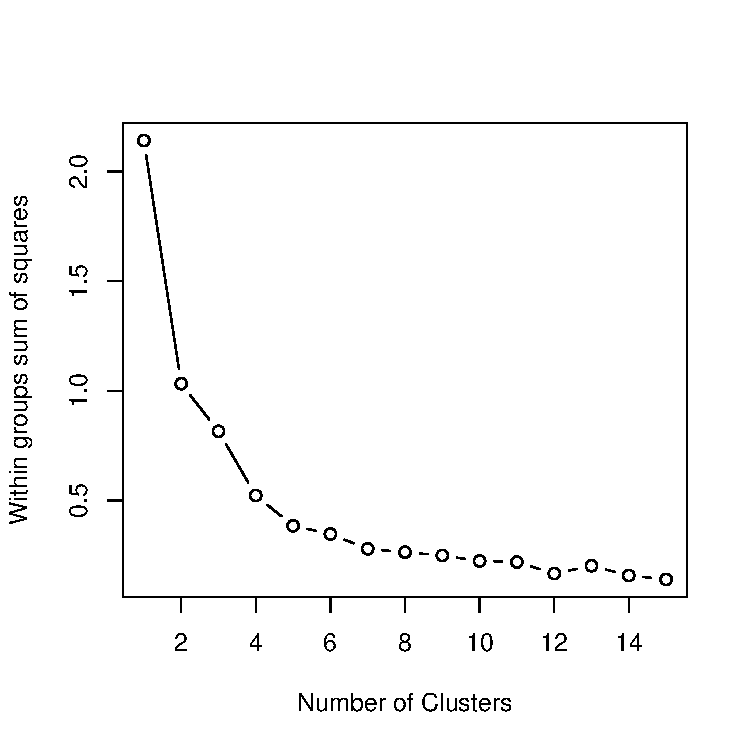
\includegraphics[width=0.6\textwidth]{Chapter_3_SWI/Figures/Supplemental_Figure_1_k_selection}
\caption[Scree plot of number of k-means clusters versus within groups sum of squares.]{k-means analysis of Loess filtered OTUs. $k = 5$ clusters was manually chosen to partition non-overlapping clusters in the network analysis.} 
\label{fig:ch2:supp2_2} 
\end{figure}

To identify OTUs with non-random temporal patterns, we first selected OTUs with a relative abundance ${\geq}$ 0.01 in at least three samples. We assessed the seasonality of this subset through local polynomial regression (LOESS) with serial day as the independent variable and relative abundance as the dependent variable, using $r^{2} > 0.8$ as a threshold to identify OTUs with non-random temporal patterns. We used these OTUs to generate a co-occurrence network based on Pearson's correlation ($r > 0.5$) using the Cytoscape (version 3.4.0; \citealt{smobwr}) CoNet plugin (version 1.1.1.beta; \citealt{faust2012microbial}). We extracted non-overlapping clusters from this network through k-means clustering using the Cytoscape clusterMaker2 plugin (version 0.9.5; \citealt{morris2011clustermaker}) after first selecting a reasonable value for k through the evaluation of a scree plot of within-clusters sum of squares (Figure \ref{fig:ch2:supp2_2}). The resulting network clusters were visualized in Cytoscape. This helped us to identify groups of OTUs with similar temporal trends.


\afterpage{
\begin{landscape}
\begin{table}[htbp]
\centering
\caption[Univariate and stepwise linear regressions of bacterial production in relation to environmental factors.]{Univariate and stepwise linear regressions of bacterial production in relation to environmental factors. Each reported $r^2$ represents a separate regression analysis.}
\label{ch2:tab1}
\begin{tabular}{@{}lllll@{}}
\toprule
Environmental factor (EF)         & Measured univariate\textsuperscript{a} $r^2$         & Interpolated univariate\textsuperscript{b} $r^2$        & Stepwise lags\textsuperscript{c} (days)       & Stepwise $r^2$       \\ \midrule
Temperature                       & 0.46                                                & 0.59                                                   & 0, 10                                        & 0.68                 \\
Phosphate                         & 0.49                                                & 0.75                                                   & NSd                                          & NS                   \\
Silicate                          & 0.29                                                & 0.53                                                   & NS                                           & NS                   \\
Nitrate+nitrite                   & 0.52                                                & 0.77                                                   & NS                                           & NS                   \\
POC                               & 0.34                                                & 0.62                                                   & 0, 10, 20                                    & 0.79                 \\
PON                               & 0.31                                                & 0.62                                                   & 0, 20                                        & 0.69                 \\
Chl \emph{a}                             & 0.23                                                & 0.25                                                   & 0, 10, 20                                    & 0.93                 \\ \midrule
                                  &                                                     &                                                        &                                              &                      \\
\multicolumn{5}{l}{\textsuperscript{a} Univariate linear regression of measured variables ($p<10^{-5}$, degrees of freedom (df)=48,}                                                 \\
\multicolumn{5}{l}{except for chl \emph{a} where $p<10^{-7}$ and df=99).}                                                                                                         \\
\multicolumn{5}{l}{\textsuperscript{b} Univariate linear regression of interpolated variables ($p<10^{-15}$, df=162, except for chl \emph{a} where df=234).}                       \\
\multicolumn{5}{l}{\textsuperscript{c} Significant lags ($p<0.001$) in the final stepwise linear regression equations based on minimized AIC are shown}                              \\
\multicolumn{4}{l}{($p<10^{-15}$, df=162, except for chl \emph{a} where df=234).}                                                                                &                \\
\multicolumn{5}{l}{\textsuperscript{d} NS is not shown due to significant multicollinearity between different lags (VIF \textgreater 5).}                                                                                
\end{tabular}
\end{table}
\end{landscape}
}

We used univariate linear regression to assess the relationships between bacterial production and abundance and environmental predictors (temperature, inorganic nutrient levels, DOC, POC, and PON) using the \code{lm} function in R \citep{t08}. Additionally, we built distributed lag models in order to account for potentially delayed bacterial responses to changes in environmental parameters \citep{jorgenson1966rational}. In order to introduce lags to our data, we first used linear interpolation as implemented in the R package \code{zoo} to predict values between sampling dates and create regular time series \citep{zeileis2005zoo}. Interpolation added data between measured time points; therefore, results were generally more significant in the analysis of interpolated data compared to measured data, as indicated by $p$-values and some cases $r^2$-values (Table \ref{ch2:tab1}, compare measured univariate $r^2$ to interpolated univariate $r^2$). However, results for regression analyses were significant based on a cut-off of $p<10^{-5}$, whether measured or interpolated data were analyzed (Table \ref{ch2:tab1}). After testing different combinations of lag, we selected the following form for distributed lag models, where \emph{BR} is a bacterial response (i.e. production or abundance) and \emph{EF} is an environmental factor:

\emph{BR $\sim$ (EF with 0-day lag) + (EF with 10-day lag) + (EF with 20-day lag)}

From this initial equation, independent variables (i.e. \emph{EF} with different lags) were selected through stepwise linear regression based on minimizing Akaike information criterion (AIC) as implemented in the R packages \code{dynlm} and \code{MASS} \citep{venables2002modern,zeileis2016dynlm}. Variables were added and removed in order of greatest reduction in AIC in a stepwise manner (i.e. backward elimination and forward selection), thereby seeking an optimal balance between goodness of fit and parameterization. Models with multicollinearity, based on variance inflation factors (VIF) > 5, were discarded. Final linear regression models were assessed for: 1) fit, 2) significance, 3) VIF, 4) AIC, and 5) parsimony.

All of our sequence data are MIMARKS-compliant \citep{Yilmaz:2011aa} and will be deposited in the NCBI SRA. Copies of the MIMARKS table and chapter figures as well as the R code used for all data analysis and figure production can be accessed at: \url{https://github.com/cmluria/dissertation/Chapter_3_SWI}. 

\section{Results}\label{results}

Our sampling period encompassed changes in day length from \textasciitilde{}4 hours of sunlight when we began sampling in July to \textasciitilde{}22 hours of sunlight in December. Water temperatures reached a minimum of \hbox{-}1.1\textdegree C in August and a maximum of 1.6\textdegree C in January (Figure \ref{fig:ch2:supp2_4}). Sea ice cover in the Palmer region is variable from year to year; 2013 was a heavy sea ice year with dense sea ice cover during the winter that persisted at significant levels until December \citep{Stammerjohn2008-nj, massom2014state}. Chl \textit{a}, a proxy for phytoplankton biomass was low (\textless{}\SI{0.6}{\micro\gram\per\liter}) until October when a brief increase in chl \textit{a} occurred. The primary phytoplankton bloom, based on chl \textit{a}, peaked in early January, after which chl \textit{a} declined towards pre-bloom levels (Figure \ref{fig:chla_bp_richness}A). Dissolved inorganic nutrients (phosphate, silicate, and nitrate) were drawn down during the summer bloom, while particulate carbon and nitrogen increased, reflecting phytoplankton production (Figure \ref{fig:ch2:supp2_4}). Silicate drawdown was less than nitrate during the summer bloom, suggesting that other phytoplankton groups in addition to diatoms contributed to the bloom. Bacterial production was very low but still detectable from July to October (Figure \ref{fig:chla_bp_richness}B). By January, bacterial production increased substantially, peaking about 3 weeks after the peak in chl \textit{a} (Figure \ref{fig:chla_bp_richness}A, B). Our bacterial production rates measured from the seawater intake were similar to those measured at a near shore station (Figure \ref{fig:ch2:bpcomp}; data available at doi:10.6073/pasta/814628d18d4e23753d1164f0bd81095e). 

While several individual factors (phosphate, silicate, nitrate and nitrite, POC, and PON) were significantly correlated with bacterial production, stepwise linear regression revealed that chl \emph{a} with time lags of 0, 10, and 20 days was a very good predictor of both bacterial production ($r^2 = 0.93$) and abundance ($r^2 = 0.62$; Figure \ref{fig:supp2_6} and Table \ref{ch2:tab1}). Adding additional lag terms to this model did not improve the fit based on $r^2$. However, removing lag terms decreased the fit (e.g., Table \ref{ch2:tab1}, compare interpolated univariate $r^2$ to stepwise $r^2$). Although we tested regressions incorporating multiple environmental factors as independent variables, the resulting models did not improve upon the distributed lag model based on chl \emph{a} alone and furthermore, often displayed multicollinearity. 

\begin{figure}[ht!] 
\centering 
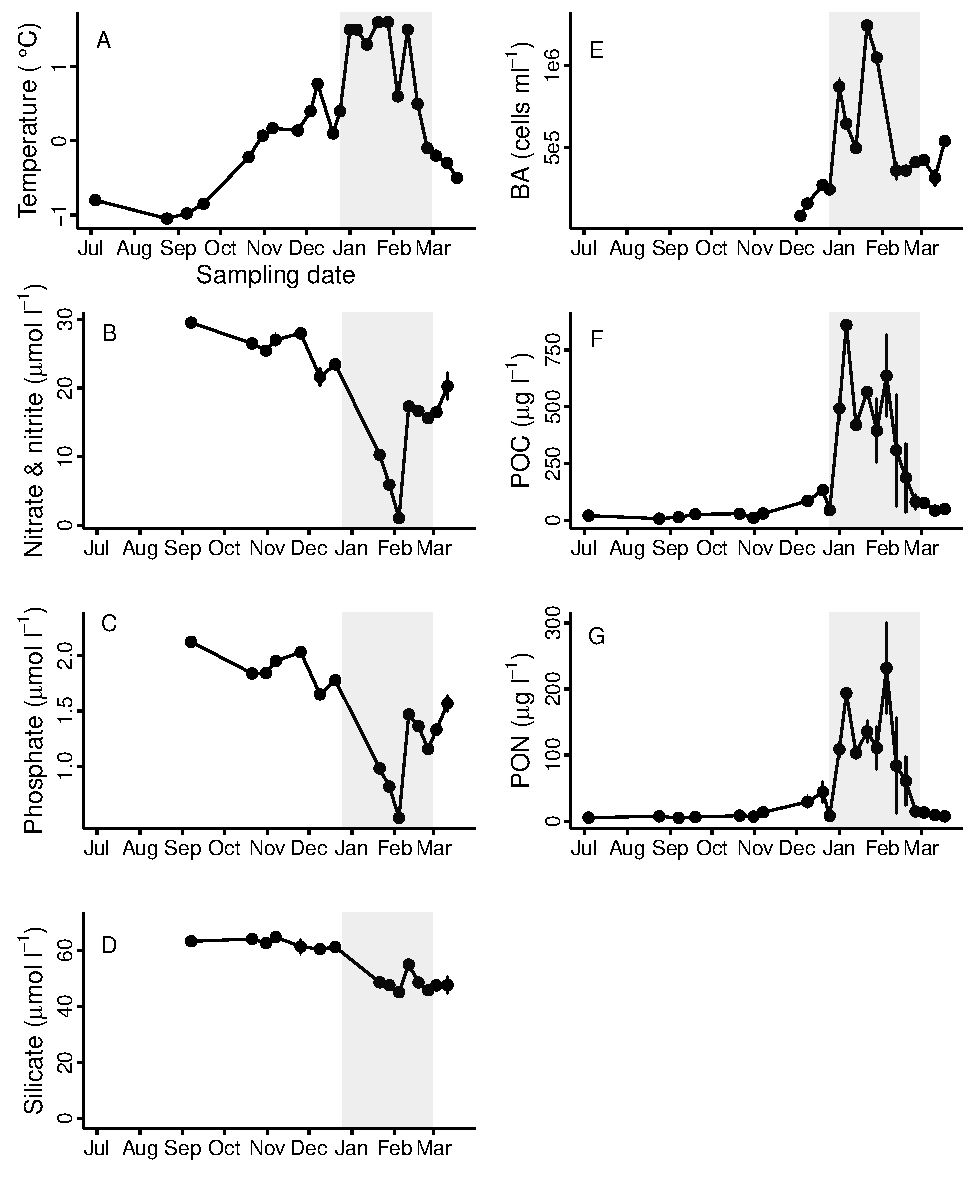
\includegraphics[width=\textwidth]{Chapter_3_SWI/Figures/Supplemental_Figure_2_ancillary_data_noDOC} 
\caption[Contextual data for bacterial community composition time series.]{Contextual data associated with sequence data including (A) temperature, (B) nitrate and nitrite, (C) dissolved inorganic phosphate, (D) dissolved silicate, (E) bacterial cell abundance (BA), (F) particulate organic carbon, and (G) particulate organic nitrogen. Mean and standard error for each time point are shown.} 
\label{fig:ch2:supp2_4} 
\end{figure}

\begin{figure}[ht!] 
\centering 
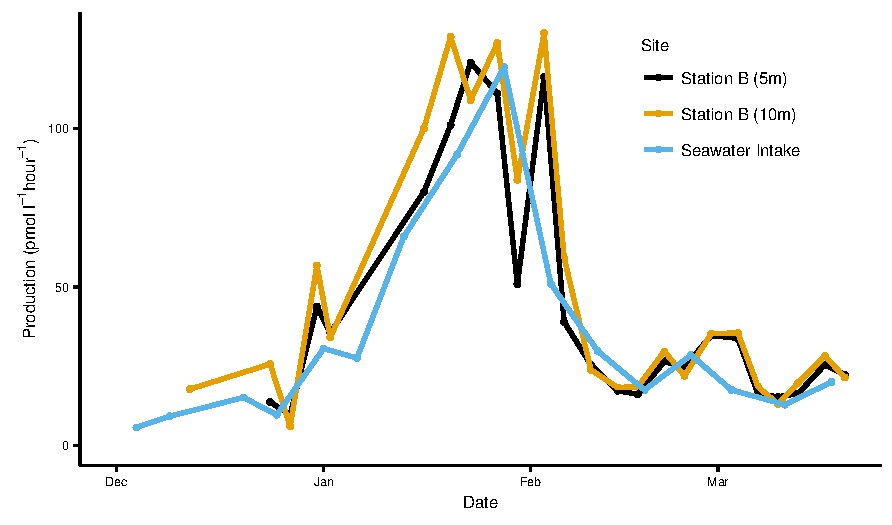
\includegraphics[width=1.0\textwidth]{Chapter_3_SWI/Figures/Supplemental_Figure_3_BP_Comparison_Across_Sites} 
\caption[Comparison of bacterial production in the Palmer Station seawater intake and at Palmer LTER Station B.]{A comparison of bacterial production from Palmer Station seawater intake and LTER Station B at 5-m and 10-m depths, December 2013-March 2014.} 
\label{fig:ch2:bpcomp} 
\end{figure}

\begin{figure}[ht!] 
\centering 
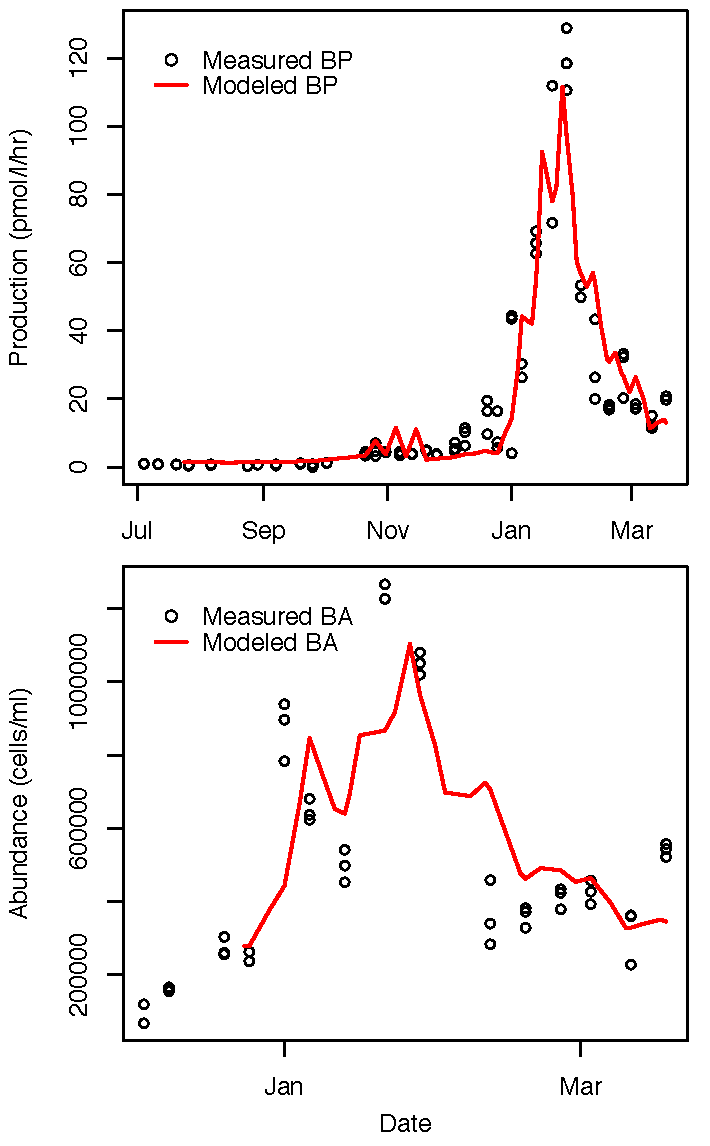
\includegraphics[width=0.6\textwidth]{Chapter_3_SWI/Figures/Supplemental_Figure_4_BP_and_BA_models} 
\caption[Measured bacterial production and abundance and values predicted through a distributed lag model.]{Measured and modeled (A) bacterial production and (B) bacterial abundance. The model fit for both production and abundance is the stepwise linear regression equation of chlorophyll \emph{a} with 0-, 10-, and 20-day lags, with minimized AIC.} 
\label{fig:supp2_6} 
\end{figure}

\begin{figure}[ht!] 
\centering 
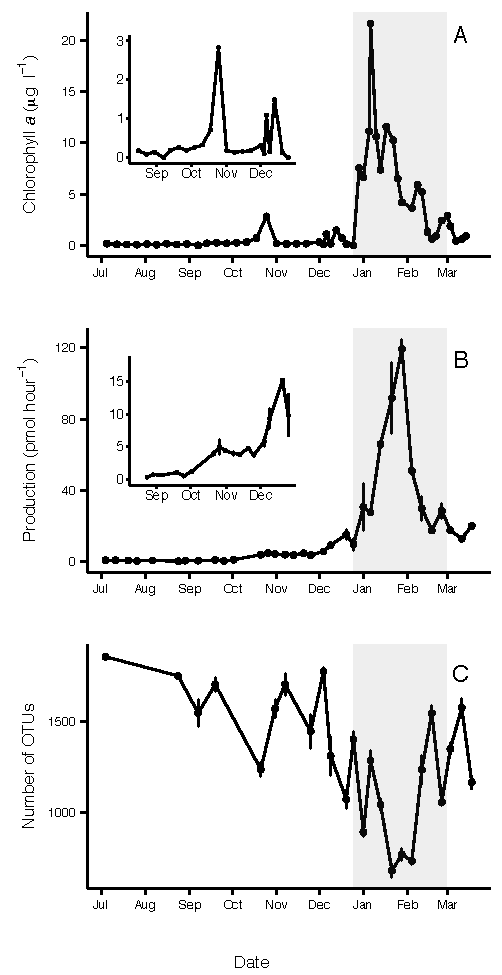
\includegraphics[width=0.6\textwidth]{Chapter_3_SWI/Figures/Figure_1_Chla_BP_richness} 
\caption[Changes in chlorophyll \emph{a}, bacterial production, and OTU richness over the nine-month time series.]{Characteristics of the summer phytoplankton bloom period (highlighted in grey), based on (A) increased chl \emph{a}, (B) increased bacterial production, and (C) decreased free-living bacterial OTU richness. Insets are shown corresponding to the time period before the summer phytoplankton bloom (A and B). Error bars represent standard error for each date.} 
\label{fig:chla_bp_richness} 
\end{figure}

In total, 68 samples, spread across 24 sampling dates, were sequenced, yielding 15 million short-read V6 16S rRNA gene sequences (\textasciitilde{}50,000-550,000 per library) corresponding to the free-living bacterial community, assigned to 28,857 OTUs. Given recent discussion regarding the statistical validity of library resampling \citep{McMurdie2014-iu}, we assessed different methods to characterize bacterial richness and community composition using un-rarefied sequence libraries. Although the method described by \citet{chao2014rarefaction} is intended to estimate true richness based on coverage regardless of sequencing depth, both OTU number ($p < 0.001, r^2 = 0.4)$ and estimated richness ($p <0.001, r^{2} = 0.35$) significantly correlated with library size (Figure \ref{fig:ch2:unrarrich}). This may indicate that the species abundance distributions vary widely among our datasets \citep{gwinn2015evaluating}. Likewise, NMDS based on un-rarefied sequence libraries showed the influence of initial library size even after relative abundance, RLE, and TMM normalizations (Figure \ref{fig:ch2:sixpanord}). For these reasons, all subsequent analyses relied on libraries rarefied to the smallest library size of 43,308 sequences.


\begin{figure}[ht!] 
\centering 
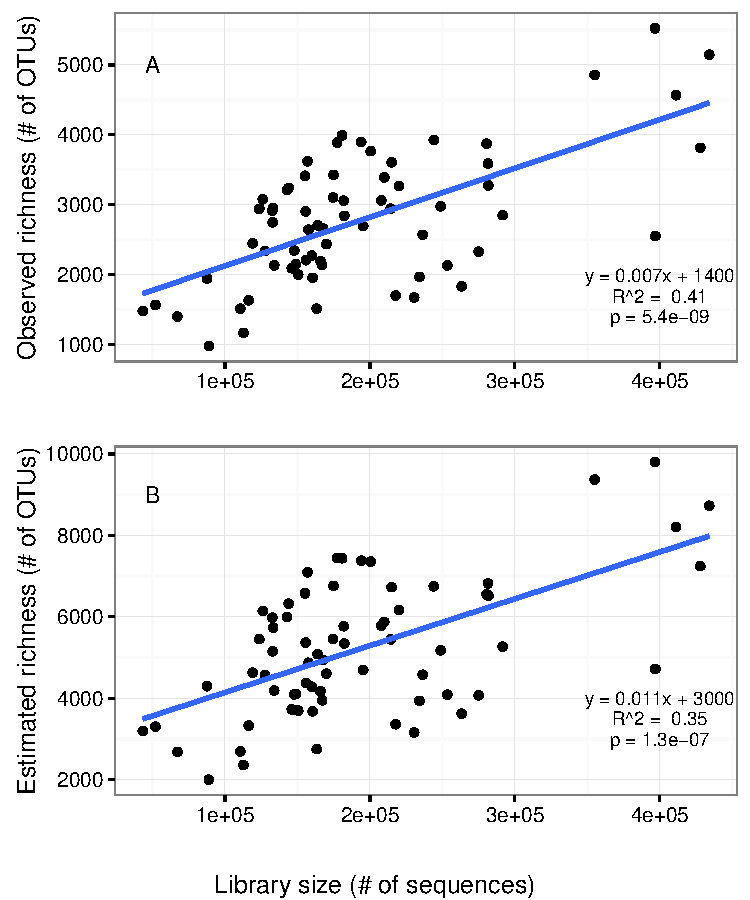
\includegraphics[width=0.7\textwidth]{Chapter_3_SWI/Figures/Supplemental_Figure_5_unrarefied_estimated_richness} 
\caption[Observed and estimated (Chao-Jost) richness versus un-rarefied library size.]{Both (A) observed richness and (B) Chao-Jost estimated richness had significant, positive correlations with un-rarefied library size.} 
\label{fig:ch2:unrarrich} 
\end{figure}

\begin{figure}[ht!] 
\centering 
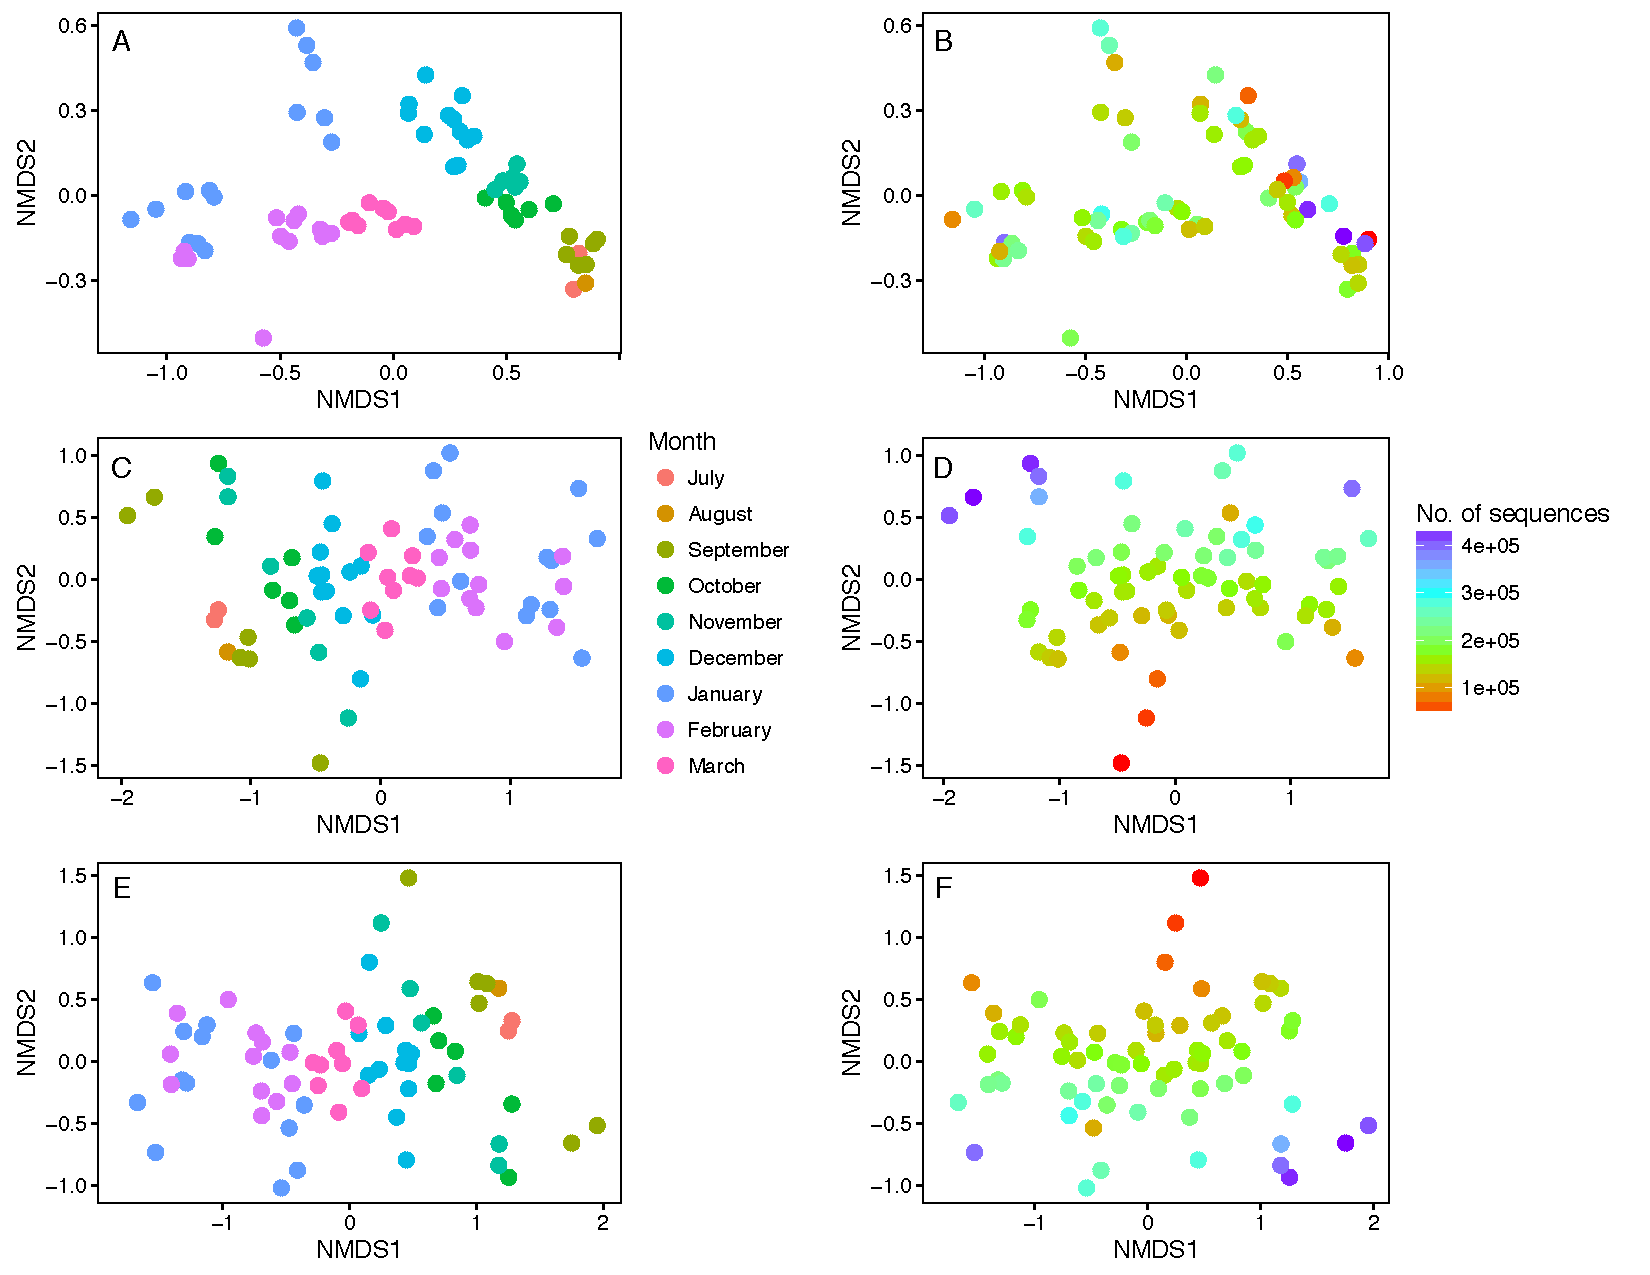
\includegraphics[width=\textwidth]{Chapter_3_SWI/Figures/Supplemental_Figure_6_Six_panel_ordination} 
\caption[Non-metric multidimensional scaling based on Bray-Curtis similarity matrices for un-rarefied libraries after three different normalization methods.]{Non-metric multidimensional scaling after running three different
normalization methods to accommodate size differences between un-rarefied libraries: simple conversion to relative abundance color-coded by month (A) and un-rarefied library size (B), Relative Log Expression (RLE) normalization (C-D), and Trimmed Mean of M-Values (TMM) normalization (E-F). Figures in left column contain samples color-coded by month. Figures in right column contain samples color-coded according to library size (number of sequences) prior to normalization.} 
\label{fig:ch2:sixpanord} 
\end{figure}


Observed richness for the free-living bacterial community varied significantly between midwinter and midsummer ($p < 0.0001$), ranging from a maximum of approximately 1800 OTUs in July to a minimum of approximately 700 OTUs in January (Figure \ref{fig:chla_bp_richness}C). On average, Chao-Jost estimated richness was four times greater than observed richness. Richness was negatively correlated with chl \emph{a} ($p<0.001, r^{2} = 0.16$) and bacterial production ($p<0.0001, r^{2} = 0.55$). A Tukey's HSD comparison across months confirmed that the decline in richness was significant in January and February ($p < 0.05$). Shannon Diversity and Pielou's evenness were also significantly lower in January ($p <0.0001$).


\begin{figure}[ht!] 
\centering 
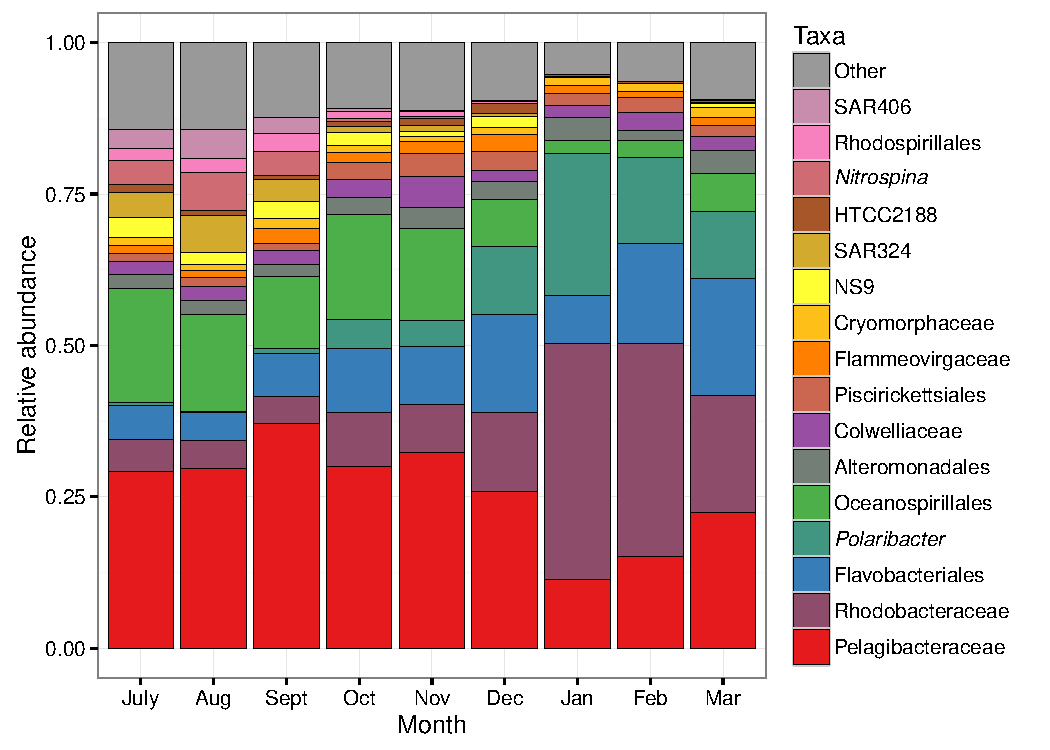
\includegraphics[width=\textwidth]{Chapter_3_SWI/Figures/Figure_2_taxa_barplot} 
\caption[Taxonomic changes in bacterial community composition over the nine-month time series.]{Taxonomic changes in free-living bacterial community composition over the 9-month sampling period. Mean relative abundance in each month is shown. Each taxon contains one or more OTUs grouped according to taxonomic assignment to genus level or higher. The lowest taxonomic level available is shown.} 
\label{fig:taxa_barplot} 
\end{figure}

Figure \ref{fig:taxa_barplot} provides a broad overview of the changes in relative abundance of free-living bacterial taxa that occurred over the course of the season. Oceanospirillales and Pelagibacteraceae were the most abundant groups in winter and spring (July-November). SAR406, Rhodospirillales, and Deltaproteobacteria, including \textit{Nitrospina} and SAR324, were present at greater relative abundances in winter and early spring (July-September) than later in the field season. Changes in the relative abundances of taxonomic groups became most evident in January when Rhodobacteraceae had greater relative abundances than Pelagibacteraceae. \textit{Polaribacter} also increased significantly in January. We did not account for variation in 16S rRNA copy number and thus may have underestimated the abundances of lower copy number taxa like Pelagibacteraceae and overestimated the abundances of higher copy number taxa like Colwelliaceae. In addition to changes in relative abundances for broad taxonomic groups, co-occurrence network analysis with k-mean clustering revealed five temporal pattern types, with individual OTUs that peaked (i) during the winter or early spring, (ii) just prior to the summer bloom, (iii) very early in the summer bloom, (iv) at summer mid-bloom, or (v) after the summer bloom subsided (Figures \ref{fig:otu_succession} and \ref{fig:ch2_network_kmeans}). Some OTUs that were assigned the same family-level classification (e.g. Rhodobacteraceae) had distinct temporal patterns corresponding to different times during the summer bloom. 


\begin{figure}[htbp] 
\centering 
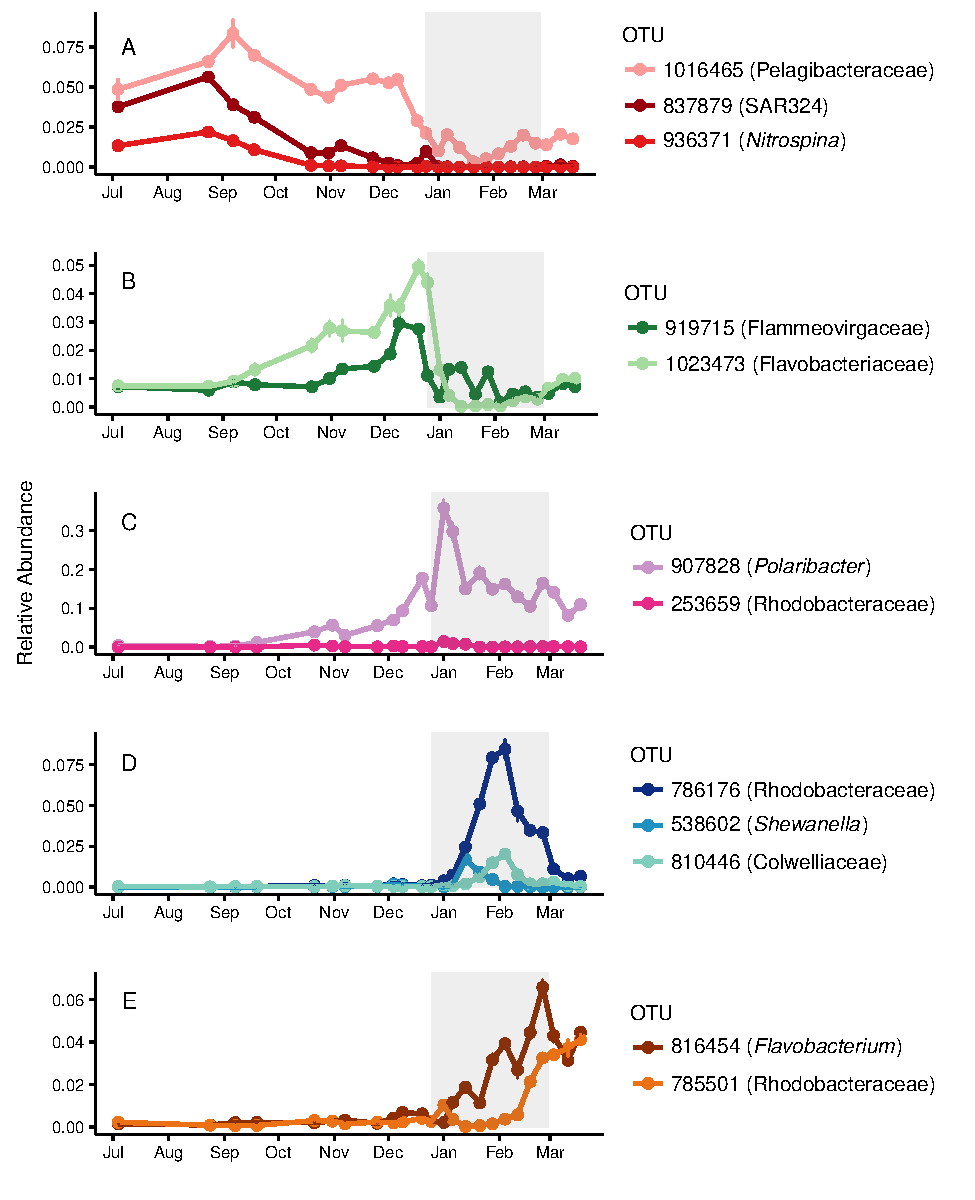
\includegraphics[width=\textwidth]{Chapter_3_SWI/Figures/Figure_3_OTU_succession_post_network_analysis} 
\caption[Five classes of successional patterns observed for individual OTUs over the nine-month time series.]{Successional patterns of free-living bacterial OTUs that peaked (A) during the winter or early spring, (B) prior to the summer bloom onset, (C) early in the summer bloom, (D) middle of the summer bloom, or (E) end of the summer bloom. Mean relative abundance and standard error for each date are shown. The affiliation of each OTU at the lowest taxonomic resolution available is shown.}
\label{fig:otu_succession} 
\end{figure}

Non-metric multidimensional scaling, based on Bray-Curtis similarities, demonstrated a shift in community composition from July through December before the onset of the summer phytoplankton bloom (Figure \ref{fig:ch2_nmds}). Community composition continued to change from December to January as the summer phytoplankton bloom developed. March samples clustered midway between the July-November and late January-early February samples, perhaps reflecting the beginning of a return to a pre-bloom community structure. PERMANOVA confirmed that community composition varied significantly between months ($p=0.$001). Bacterial communities fell into five groups based on hierarchical clustering of Bray-Curtis similarities. These groups corresponded to different time periods and ranges of bacterial production: July to November (winter and spring; \textless{} \SI{5}{\pico\mole \per\liter \per\hour}), December and March (before and after the summer bloom; \SIrange{5}{21}{\pico\mole \per\liter \per\hour}), early January (beginning of the summer bloom; \SIrange{26}{44}{\pico\mole \per\liter \per\hour}), late January to early February (summer mid-bloom; \SIrange{50}{129}{\pico\mole \per\liter \per\hour}), and late February (late in the summer bloom; \SIrange{17}{43}{\pico\mole \per\liter \per\hour}).

\begin{figure}[htbp] 
\centering 
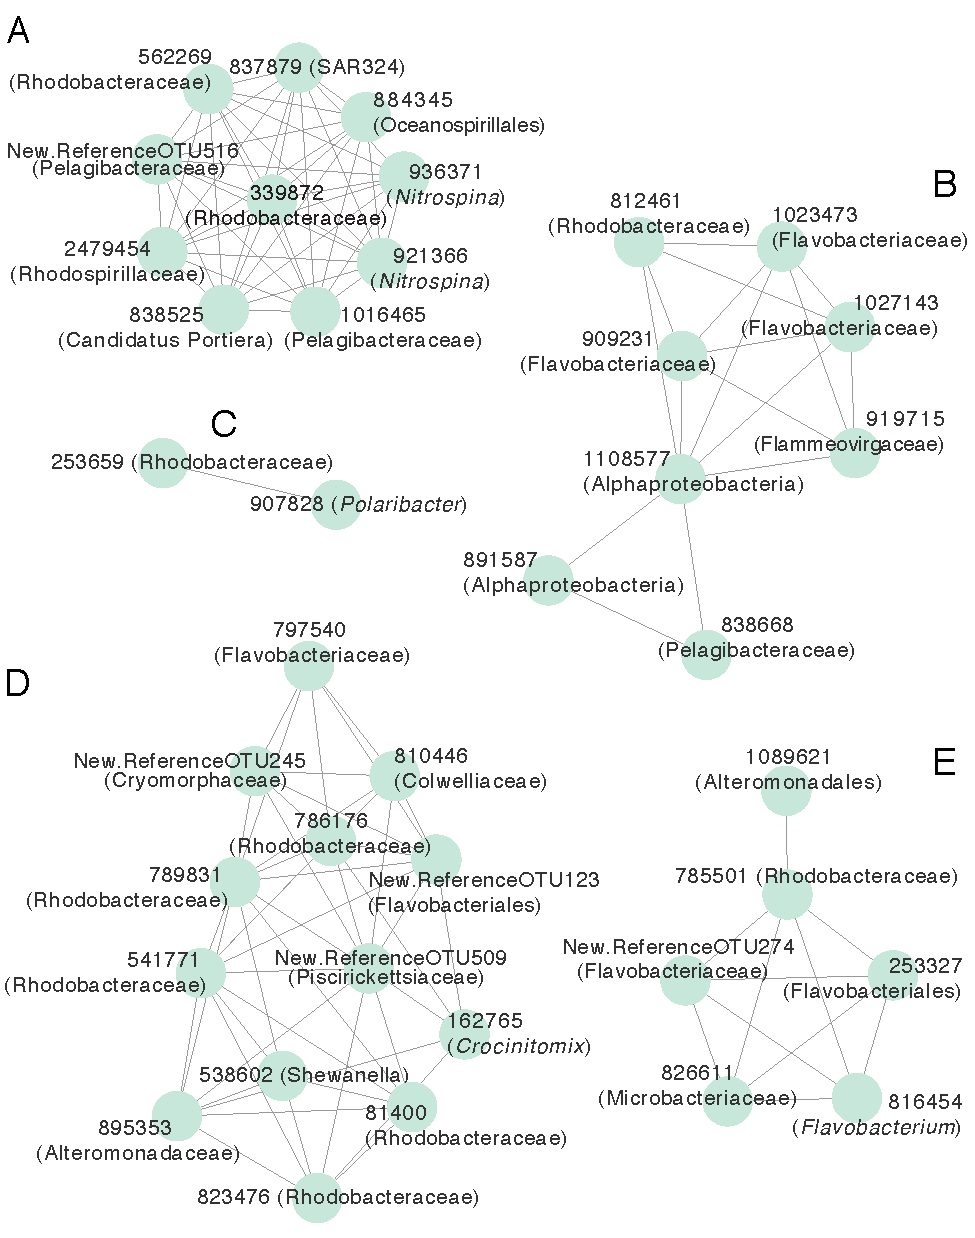
\includegraphics[width=0.8\textwidth]{Chapter_3_SWI/Figures/Figure_4_otu_network_LoessPrefilter_kmeans_Pearsons} 
\caption[Co-occurrence networks of OTUs that displayed strong temporal patterns in relative abundance.]{Correlation network of free-living bacterial OTUs with strong temporal patterns in relative abundance, based on Pearson's correlation ($r > 0.5$) of LOESS-filtered OTUs. OTUs were partitioned into non-overlapping clusters using k-means clustering ($k = 5$).${~}$Edges represent positive correlations and nodes represent individual OTUs, labeled with OTU identification number and lowest level of taxonomic resolution available. The letters designate clusters that represented OTUs that peaked (A) during the winter or early spring, (B) prior to the summer bloom onset, (C) early in the summer bloom, (D) middle of the summer bloom, or (E) end of the summer bloom. Representative OTUs from each cluster are shown in Figure \ref{fig:otu_succession}.} 
\label{fig:ch2_network_kmeans} 
\end{figure}

\begin{figure}[htb!] 
\centering 
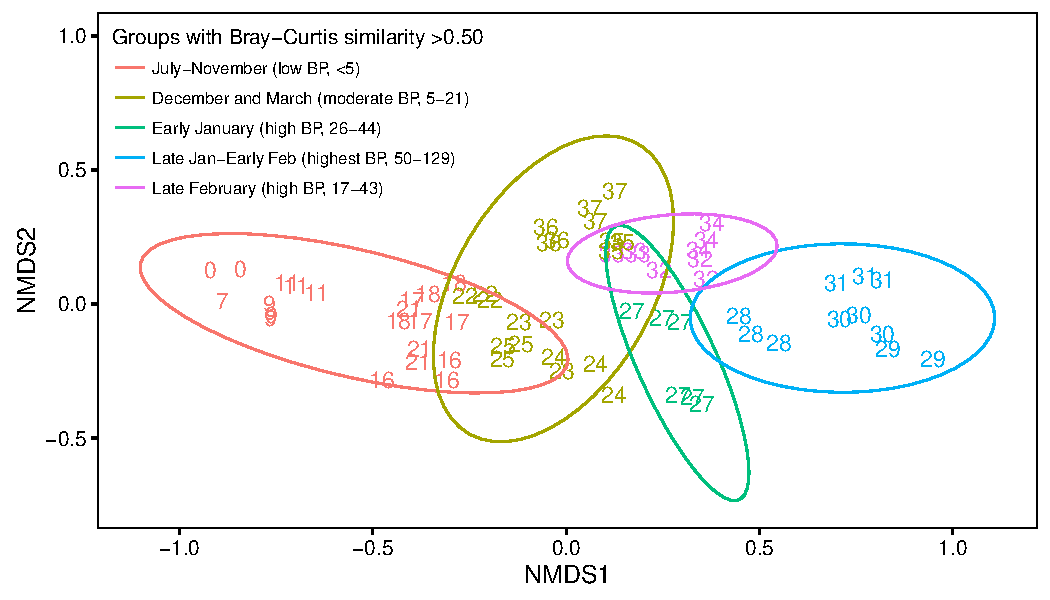
\includegraphics[width=0.9\textwidth]{Chapter_3_SWI/Figures/Figure_5_NMDS} 
\caption[Non-metric multidimensional scaling (NMDS) of Bray-Curtis similarity indices based on OTU relative abundance.]{Non-metric multidimensional scaling of Bray-Curtis similarity indices of free-living bacterial community composition based OTU relative abundance. Number labels indicate when the sample was collected in weeks since the initial sampling date in July. Identical number labels indicate three replicate samples collected at the same time, except in week 27 (early January) when replicate samples were collected on two separate days. Not every week was sampled during the study period, as indicated by number labels. Color indicates different groups according to hierarchical clustering with a Bray-Curtis similarity cut-off of 0.5. Ellipses represent the 0.95 confidence interval for each Bray-Curtis similarity group. The time period and range of bacterial production (BP) corresponding to each Bray-Curtis similarity group are shown. } 
\label{fig:ch2_nmds} 
\end{figure}

\section{Discussion}\label{discussion}

We observed a significant decline in free-living bacterial OTU richness as bacterial production increased during the midsummer phytoplankton bloom. Previous studies of temperate systems have also reported diversity maxima in the winter and minima in the summer \citep{Gilbert2012-ta, Ladau2013-ro}. Similar seasonal trends in bacterial OTU richness have been reported at a much lower resolution in Antarctic waters \citep{Ghiglione2012-qm,Georges2014-ng,grwddecm12,Luria2014-dj}. \citet{Gilbert2012-ta} observed relatively gradual changes, reporting that day length and serial day alone explained over 66\% of the observed variance in richness during a 6-year time series study of the English Channel. Likewise, during a six-year study in the Northwest Atlantic Ocean, \citet{El-Swais2015-yx} observed a much longer period of decreased richness during the summer and spring that accompanied an extended period of increased primary production. In contrast, we observed only a brief period (\textasciitilde{}4 weeks) of decreased richness that coincided with increased bacterial production rates. The abbreviated nature of phytoplankton blooms in the WAP along with high-resolution temporal sampling, enabled us to observe this pattern, which contrasts with the multiple annual blooms and/or long periods of sustained growth seen in temperate systems. The results of our study demonstrate close temporal linkages between episodic but biologically significant events like phytoplankton blooms and bacterial production and richness. 

In addition to changes in alpha diversity, we measured temporal variation in the taxonomic composition of free-living bacterial communities. The most abundant winter bacterial taxonomic group in our amplicon sequence data was Pelagibacteraceae, a globally abundant clade that correlates negatively with primary production \citep{Morris2002-xb,Sowell2009-oc}. Several bacterial taxa involved in alternative energetic pathways, e.g. SAR406 (sulfur oxidation; \citealt{wright2014genomic}), \textit{Nitrospina} (nitrite oxidation; \citealt{Spieck2014-sp}), and SAR324 (sulfur oxidation and carbon fixation; \citealt{Sheik2014-yg}) dominated early in the winter, in accordance with previous suggestions that chemolithoautotrophy is an important metabolism contributing to cellular production during the winter \citep{grwddecm12,williams2012metaproteomic,manganelli2009major}. Although we did not sequence archaea in this study, ammonia-oxidizing Thaumarchaeota contribute significantly to chemolithoautotrophy during winter, and overall ammonia oxidation rates are higher in winter than summer \citep{tolar2016contribution}. The seasonality in \textit{Nitrospina} may be related to changes in ammonia oxidation rates. 

While species richness did not change significantly until the phytoplankton bloom in summer, free-living bacterial community composition began to change as early as October, with declining relative abundances of Pelagibacteraceae, SAR406, SAR324, and \textit{Nitrospina}. As the season progressed, increasing competition or top-down control may have caused declines in the relative abundances of these taxa, while increasing water temperatures and therefore increased water column stratification would have prevented replenishment of taxa from deeper waters. The increased relative abundances of taxa like Flavobacteriaceae, \textit{Polaribacter}, Flammeovirgaceae, and Rhodobacteraceae before the summer phytoplankton bloom is somewhat surprising given the low levels of chl \textit{a} and bacterial production during this time period. A brief increase in chl \textit{a} in late October coincided with a decline in richness and an increase in bacterial production. While richness increased when chl \textit{a} subsided, bacterial production remained slightly elevated over the next two months. These pre-summer changes in community composition could reflect a direct response by certain bacterial taxa to increasing sunlight, in addition to low-level and ephemeral increases in phytoplankton. For example, some marine Flavobacteria, including \textit{Polaribacter}, contain proteorhodopsin, a light-driven proton pump that can enhance growth in low-nutrient conditions, while Rhodobactaceae have been shown to carry out aerobic anoxygenic photosynthesis \citep{gonzalez2008genome,Kimura2011-eh,Xing2015-kz,Voget2015-ch}. Whether or not pre-summer changes in bacterial community composition are associated with bacterial feedbacks on phytoplankton growth is not known \citep{Amin2012-tv,Amin2015-pp,Prieto2015-oi,Wang2016-lt}. 

As the summer phytoplankton bloom developed, we observed changes in community composition that corresponded to changes in bacterial production. The relative abundance of free-living \textit{Polaribacter} doubled while that of Rhodobacteraceae tripled during the phytoplankton bloom. We noted that different OTUs within Flavobacteriaceae, including \textit{Polaribacter}, and Rhodobacteraceae peaked at different points during the phytoplankton bloom. This suggests niche specialization by different taxa within these groups, perhaps corresponding to different stages in the successive degradation of phytoplankton-derived organic compounds \citep{Teeling2012-jz,Klindworth2014-ba}. \textit{Polaribacter} occurred in a cluster with only one other OTU (Figure \ref{fig:otu_succession} and \ref{fig:ch2_network_kmeans}), suggesting a strong competitive advantage for \textit{Polaribacter} early in the bloom, in support of the hypothesized role of this taxon \citep{williams2013role}. Rhodobacteraceae OTUs that peaked later in during the bloom may utilize secondary products of decomposing organic matter, such as low molecular weight compounds \citep{Voget2015-ch}. We observed a mid-bloom increase in the relative abundance of Gammaproteobacteria, including \textit{Shewanella} and Colwelliaceae, taxa previously associated with substrate rich environments \citep{Baelum2012-re,Delmont2014-ng}. Early February peaks in the abundance of OTUs classified as Rhodobacteraceae and Colwelliaceae corresponded to almost complete depletion of nitrate and nitrite, an unusual event in the WAP that might have caused phytoplankton to release carbohydrates \citep{hansell2014biogeochemistry}. It is important to note that our focus on the <\SI{3.0}{\micro\meter} fraction of the bacterial community excluded particle-associated bacteria, that may have played an increasingly important role as the phytoplankton bloom developed \citep{riemann2000dynamics}.

We used distributed lag models to statistically test the dynamic relationship between phytoplankton abundance based on chl \textit{a} and bacterial production and abundance during this period. The inclusion of 10- and 20-day lags in our model allowed us to capture a greater portion of the variability in these relationships. In January, peak bacterial production occurred about 20 days after the peak in chl \textit{a}, in agreement with previous studies of Antarctic phytoplankton bloom dynamics \citep{billen1991phytoplankton,ducklow2001seasonal}. A secondary chl \textit{a} peak in mid-January would have presumably also contributed to the peak in bacterial production that occurred about 10 days later.${~}$Bacterial reliance on high molecular weight phytoplankton-derived organic matter that must undergo extracellular hydrolysis prior to bacterial uptake is thought to drive such temporal lags \citep{billen1991phytoplankton,ducklow2001seasonal,lancelot1991modelling,kirchman2001glucose}. Furthermore, some DOM fractions may become available through intermediate trophic processes (e.g. zooplankton sloppy feeding or excretion; \citealt{dsvse12}). The significance of both 10- and 20-day lags may reflect the complex nature of WAP DOM degradation, in which individual bacterial taxa respond within different time frames and specialize in different fractions of the DOM pool \citep{nikrad2014uptake,bowman2015microbial,kim2016decedal}.

We hypothesize that resource supply from phytoplankton-derived carbon was the primary factor driving the summertime shift in free-living bacterial community composition, although biotic interactions and top-down control by grazing and viral lysis likely modulate the patterns that we observed \citep{bird1999uncoupling,Brum2016-ig}. Our measurements did not directly address the underlying mechanisms controlling temporal patterns in bacterial community composition. In particular, we did not directly measure the composition or turnover of organic compounds that we hypothesize contributed to changing bacterial communities. Our study and other similar studies also lack a multi-year dimension to be definitive. Nevertheless, the general pattern that we observed is consistent with the view that increased resource supply of a diverse pool of organic compounds that results from phytoplankton blooms plays a strong role in structuring bacterial communities \citep{Teeling2012-jz,Buchan2014-yh}. 

Taken together, our bacterial production, richness, and community composition data indicate strong trophic coupling between bacteria and phytoplankton. Our results agree with previous reports that WAP bacterial density and production are positively correlated with primary production \citep{Church2003-oj,Ortega-Retuerta2008-pk}, but contrast with earlier reports that the microbial loop is uncoupled from primary producers during spring phytoplankton blooms \citep{Bird1991-sx,bird1999uncoupling,Karl1991-cs,duarte2005experimental}. Although community shifts like those we observed suggest strong potential for degradation of labile phytoplankton-derived organic matter \citep{Landa2014-yg}, WAP bacterial standing stocks and productivity are low relative to primary production (\textasciitilde{}5\% versus 10-20\% global average; \citealt{dsvse12,kim2016decedal}). Despite the longstanding debate about the role of temperature in limiting bacterial production in cold water, several analyses found that temperature is not the principal factor regulating bacterial growth in the Antarctic \citep{dsvse12,thingstad1991bacteria,Kirchman2009-sg}. However, there is growing evidence, including results from this study, that labile organic matter availability is a primary factor controlling bacterial growth and community composition in Antarctica \citep{Kirchman2009-sg,dsvse12,kim2016decedal}. 


 
\chapter{Influence of phytoplankton-derived dissolved organic matter on marine bacterial community dynamics on the Western Antarctic Peninsula}\label{ch:dom}

\chapterdisclaimer{This work was performed in collaboration with Linda Amaral-Zettler, Hugh Ducklow, Daniel Repeta, Andrew Rhyne, and Jeremy Rich.\\
\\
Catherine Luria, Linda Amaral-Zettler, Hugh Ducklow, and Jeremy Rich designed and conducted the study with assistance from Dan Repeta and Andrew Rhyne. Linda Amaral-Zettler and Jeremy Rich contributed sequence data for the study. Catherine Luria analyzed data and wrote this chapter with guidance from Jeremy Rich. 
}


\section{Abstract}

Bacterial interactions with dissolved organic matter (DOM), largely produced by phytoplankton, drive much of the movement of carbon through the oceanic food web and the global carbon cycle. The extent to which DOM, especially phytoplankton exudates, drives bacterial community assembly is unclear and describing the complex interactions between bacteria and marine DOM remains an important challenge. The marine ecosystem of the Western Antarctic Peninsula (WAP) undergoes a dramatic seasonal transition each spring that culminates in intense summer phytoplankton blooms, providing a dynamic system in which to study these interactions. We tested the hypothesis that WAP bacterial growth and community succession are primarily driven by the availability of labile DOM  through a series of mesocosm experiments that spanned the WAP spring transitional period (August-December 2013). The addition of DOM, in the form of cell-free exudates extracted from \emph{Thalassiosira weissflogii} diatom cultures to 50-L mesocosms led to changes in bacterial abundance, production, and community composition. The timing of each experiment (i.e. early spring versus late spring) influenced the magnitude and direction of these changes. For example, the same DOM treatment applied at different times during the season resulted in different levels of bacterial production and different bacterial community composition, including a striking mid-season shift between Colwelliaceae and \emph{Polaribacter}. Our findings suggest that the timing of phytoplankton blooms can alter bacterial community response, perhaps indicating the influence of priority effects. Strong interannual variability as well as long-term climate change may shift the timing of WAP phytoplankton blooms and bacterial responses to this shift could have profound implications for the bacterial-mediated movement of carbon and nutrients through the WAP ecosystem.

\section{Introduction}

Marine dissolved organic matter (DOM) represents the largest exchangeable reservoir of carbon on Earth and drives a considerable fraction of the oceanic food web \citep{hedges1992global}. Phytoplankton production is the dominant source of marine organic material, with an estimated 50\% of algal production entering the DOM pool through a variety of mechanisms \citep{lampert1978release,fogg1983ecological,gobler1997release}. The resulting DOM pool is a complex mixture of thousands of organic compounds with varying degrees of lability. Over 90\% of the material released by algae is considered labile and is consumed and respired within days; meanwhile, a wide variety of more recalcitrant compounds accumulate in seawater and are available for long-term sequestration in the deep ocean \citep{ducklow2001seasonal}. Despite long-term ramifications for atmospheric \ce{CO_2} concentrations, the interplay between diverse bacterial assemblages and complex DOM pools is poorly understood. 

 

Phytoplankton blooms are associated with shifts in bacterial community composition \citep{Pinhassi2004-kc,Teeling2012-jz,Klindworth2014-ba}, perhaps due to changes in DOM availability and composition. Previous studies provide conflicting reports of generalist assemblages that can utilize a wide variety of substrates \citep{mou2007bacterioplankton,newton2010genome,chronopoulou2015generalist} as well as communities of specialists that are adapted to take advantage of only certain classes of DOM compounds and respond quickly to disturbance \citep{cottrell2000natural,am08,nelson2012tracking,sarmento2012use,Klindworth2014-ba,sharma2014distinct}. Nonetheless, some general trends based on broad taxonomic groups have emerged. For example, certain groups of bacteria (e.g., Flavobacteria and Rhodobacteraceae) tend to increase in abundance during phytoplankton blooms, while other groups such as \emph{Pelagibacter} appear better adapted to non-bloom conditions \citep{williams2013role,Buchan2014-yh,Voget2015-ch}. 

 

The Western Antarctic Peninsula (WAP) provides a dynamic environment in which to study bacterial response to phytoplankton blooms. The WAP system undergoes an extreme seasonal transition every spring, from almost total darkness to almost continuous sunlight, resulting in a synchronized cascade of environmental changes that culminates in intense phytoplankton blooms, supporting a highly productive food web \citep{Venables2013-me,Smetacek2005-tz}. Bacterioplankton activity closely follows the annual phytoplankton cycle and bacterial growth and succession are thought to be largely driven by DOM availability \citep{Kirchman2009-sg,dsvse12}, the relationship between phytoplankton-derived DOM and bacteria has not been directly tested. Furthermore, the WAP is subject to strong inter-annual variability in sea ice and upper water column dynamics, while dramatic warming of the WAP region over the last 50 years has reduced sea ice extent and led to earlier sea ice retreat in the spring \citep{saba2014winter,vaughan1996recent,mk05,thomas2009ice,Stammerjohn2008-nj}. It is not known how changes in the timing of sea ice retreat, and subsequently of phytoplankton blooms, may alter bacteria-DOM interactions and carbon cycling. 

We conducted a series of DOM-addition mesocosm experiments that spanned the WAP spring transitional period to examine how pre-bloom communities react to changes in DOM availability. While many previous DOM-addition experiments have relied upon relatively simple compounds (e.g. glucose or amino acids), which may be poor analogs for the organic carbon utilized by marine bacteria in the WAP \citep{dmegm11,straza2010abundance}, we used diatom exudates, a more complex substrate. Our goals were to assess how diatom exudates alter the bacterial community and how these alterations change depending on the timing of the experiment in relation to the season. We hypothesized that DOM additions would change bacterial community composition and that the magnitude of these DOM-driven changes would decrease as the season progressed and organic carbon availability increased in the environment. 

 

\section{Methods}

\subsection{DOM preparation} 

Large-scale (500L) axenic cultures of \emph{Thalassiosira weissflogii}, a well-characterized marine diatom, were grown in f/2 medium \citep{f2guillard1975} in custom acid-washed polycarbonate containers. The cultures were harvested at seven days when they had developed dense growth but were still in the exponential growth phase. Previous work shows that \emph{T. weissflogii} DOM exudates collected at this stage are primarily comprised of carbohydrates, acetate, and lipids and are enriched for carbohydrates relative to seawater \citep{aluwihare1999comparison}. The create an f/2 "control," the same volume of f/2 media was treated identically, but was not inoculated with \emph{T. weissflogii}. This control was to account for any DOM in the f/2 seawater itself. 

Cells and particulate matter were removed via peristaltic pump-driven serial filtration through combusted GF/F filters (Whatman, GE Healthcare Life Sciences, Piscataway, NJ, USA) and acid-washed \SI{0.2}{\micro\meter} polyethersulfone membrane filter capsules (Whatman, GE Healthcare Life Sciences, Piscataway, NJ, USA) using acid-washed platinum-cured silicon tubing (Masteflex, Cole Parmer, Vernon Hills, IL). The filtrate was collected in clean acid-washed polycarbonate containers, acidified by adding sufficient hydrochloric acid to lower the pH to \textasciitilde{}5.0, and stored in the dark until further processing. 

Solid phase extraction of DOM, which has been shown to capture \textasciitilde{}60\% of marine DOM on average \citep{dittmar2008simple}, was performed by pumping the filtrate through C18 HPLC columns (Cole Parmer, Vernon Hills, IL) at a rate of 50 ml min$^{-1}$. The columns were prepared by gravity-driven flushing with 100 ml methanol followed by 200 ml of MilliQ water (EMD Millipore, Merck KGaA, Darmstadt, Germany). DOM was eluted from the C18 columns into combusted roundbottom flasks by flushing the columns with 100 ml of methanol. The DOM solution was gently warmed to 35 \textdegree C and was concentrated by vacuum evaporation followed by flushing with nitrogen gas as needed, leaving a dried residue suitable for transport. Aliquots of the DOM solution were retained to measure DOC concentration on a Shimadzu TOC analyzer (Shimadzu, Inc., Columbia, MD). 

Prior to mesocosm experiments, the dried DOM was re-dissolved in a \SI{0.2}{\micro\meter}-filtered 10 mM sodium hydroxide solution. The solution was centrifuged for 15 minutes at 3240 rpm to remove any particulate matter, which was retained, dried, and weighed to re-calculate the DOC concentration and make necessary amendment volume adjustments. 

 

\subsection{Mesocosm experiments}

Mesocosm experiments were conducted in August, September, October, and December 2013 at Palmer Station, Antarctica. Acid-washed 50 L polycarbonate carboys were filled directly from a seawater intake located at a depth of 6 m, 16 m from the shore. The intake was sampled prior to any filtering on station. The collected water was divided into two groups: (1) control (no additions, $n=3$) and (2) +DOM (\SI{40}{\micro\mole} DOM addition; $n=3$). An additional f/2 control treatment ($n=3$) was included in the October experiment. The carboys were incubated for 10 days under \emph{in situ} temperatures and continuous light with PAR levels inside the carboys of \SI{1e15}{quanta~\cm^{-2}~\second^{-1}} inside carboys).

Chlorophyll \emph{a} (chl \emph{a}) and phaeopigment, dissolved organic carbon (DOC), dissolved inorganic nutrients (phosphate, silicate, nitrite and nitrate), and bacterial production ($^{3}$H-leucine incorporation rates) were assessed every 48 hours for 10 days using methods previously described in Chapter 3. Bacterial abundance samples were also collected every 48 hours and were analyzed by flow cytometry with SYBR \textsuperscript{\textregistered} Green I nucleic acid staining (Invitrogen, Carlsbad, CA) on a Guava easyCyte flow cytometer (EMD Millipore, Billerica, MA). Samples for bacterial community composition were collected on days 0, 6, and 10 by filtering \textasciitilde{}2L water through successive \SI{3.0}{\micro\meter} polycarbonate and \SI{0.22}{\micro\meter} polyethersulfone (EMD Millipore, Billerica, MA) filters. Filters were flash-frozen with liquid \ce{N_2} and stored at -80\textdegree C until further processing. Samples for particulate organic carbon (POC) and particulate organic nitrogen (PON) were collected on days 0 and 10 as described in Chapter 3. All sampling took place at incubation temperatures. 

 

\subsection{16S rRNA gene library generation} 

Sequence libraries were generated as in \citet{Eren2013-ob}, with modifications as described in Chapter 3. Briefly, DNA was extracted from cells captured on the \SI{0.22}{\micro\meter} pore size filters (i.e. "free-living" bacterioplankton) using a DNeasy Plant Mini Kit (Qiagen, Valencia CA) with an additional bead-beating step. For each DNA sample, the V6 hypervariable region of the 16S rRNA gene was amplified by polymerase chain reaction (PCR) with custom fusion primers that contained Illumina adaptors and inline barcodes (forward primer) or dedicated indices (reverse primer) \citep{Eren2013-ob}. Size-selected PCR products were quantified and pooled in equimolar amounts prior to sequencing on one lane of an Illumina HiSeq 1000 cycle paired-end run. 

Low-quality sequences were filtered from the resulting data by discarding reads without 100\% consensus between forward and reverse paired-end sequencing reads \citep{Eren2013-ob}, resulting in more than 16 millions sequences across 81 libraries. OTUs were clustered using Qiime (v 1.9.1; \citealt{Caporaso2010-ee}) with open reference OTU picking with the default UCLUST method (Edgar 2010), a minimum cluster size of 2, and a 97\% similarity threshold and were assigned Greengenes taxonomy (version 13\_8; \citealt{McDonald2012-qf}). After removing OTUs classified as Chloroplasts, rarefied libraries were produced by randomly down-sampling to the smallest library size of 64271 sequences spread among 14751 OTUs. All of our sequence data are MIMARKS-compliant \citep{Yilmaz:2011aa} and will be deposited in the NCBI Sequence Read Archive. 

\subsection{Data analysis}

We estimated community turnover rate by dividing carbon biomass, derived from bacterial abundance with a conversion factor of \SI{e-14}{\gram} C per cell, by the rate of carbon uptake, derived from bacterial production measurements with a conversion factor of 1500 g C per mole \ce{^3H}-leucine incorporated. To separate the effects of experiment month, experiment day (i.e. days into incubation period), and treatment on environmental parameters, we used ANOVA to compare linear models based on different combinations of independent variables using the \code{lm} and \code{anova} functions in R \citep{t08}. 

Alpha diversity metrics, including the number of OTUs observed in each library, Shannon's diversity, and Pielou's evenness, were calculated using the \code{BiodiversityR} package in R \citep{kindt2005tree}. The beta diversity between samples was visualized with non-metric multidimensional scaling (NMDS) based on Bray-Curtis similarity using the \code{metaMDS} function in the \code{vegan} R package \citep{Oksanen_2015}. Co-occurrence network analyses based on Pearson's correlations revealed relationships among OTUs and between OTUs and external variables (i.e. experimental treatments and bacterial production). Networks were generated using the Cytoscape CoNet plugin (version 1.1.1.beta; \citealt{faust2012microbial}) and were visualized in Cytoscape (version 3.4.0; \citealt{smobwr}). Copies of the MIMARKS table and chapter figures as well as the R code used for all data analysis and figure production can be accessed at: \url{https://github.com/cmluria/dissertation/Chapter_4_DOM}. 

\section{Results}

Our experiments spanned the winter-to-late spring period, which was characterized by relatively consistent environmental conditions before the onset of an intense phytoplankton bloom in January, described in Chapter 3. Chl \emph{a} remained quite low, below \SI{1}{\micro\gram \per\liter} in the environment except for brief increase to \SI{2.8}{\micro\gram \per\liter} that corresponded to the onset of our October experiment, compared to a peak in chl \emph{a} of \textasciitilde{}\SI{20}{\micro\gram \per\liter} during the summer bloom (Figure \ref{fig:ch3:swi}  and \ref{fig:ch3:chla_poc_pon} ). During our experimental period (August - December 2013), temperatures increased steadily from -1.2 to 0.8\textdegree C. Sea ice persisted into December, beyond our last experiment, and water column light availability would have been relatively low \citep{massom2014state}. Inorganic nutrients (nitrate and nitrite, phosphate, silicate) were somewhat lower in October, corresponding to the brief increase in chl \emph{a}, but were never depleted (Figure \ref{fig:ch3:swi}  and \ref{fig:ch3:nutrients} ). DOC increased from \textasciitilde{}\SI{40}{\micro\mole} in August to \textasciitilde{}\SI{60}{\micro\mole}  in December. POC increased from \textasciitilde{}\SI{10}{\micro\gram \per\liter}  at the onset of the first experiment to \textasciitilde{}\SI{70}{\micro\gram \per\liter}  at the onset of the last experiment, but this increase is minor relative to the \SI{800}{\micro\gram \per\liter}  recorded during the January phytoplankton bloom. There was a slight enrichment of POC at the beginning of the experiments in DOM+ mesocosms, corresponding to \textasciitilde{}10\% of added DOC (Figure \ref{fig:ch3:swi}  and \ref{fig:ch3:chla_poc_pon}). While bacterial abundance was fairly stable, bacterial production increased slightly, from {\textless}\SI{1}{\pico\mole \per\liter \per\hour} to \textasciitilde{}\SI{5}{\pico\mole \per\liter \per\hour}  during the experimental period, compared to a peak of \textasciitilde{}\SI{120}{\pico\mole \per\liter \per\hour}  during the January bloom (Figure \ref{fig:ch3:environment_BA_BP_turnover}). This increase was associated with a doubling of the community turnover rate (Figure \ref{fig:ch3:environment_BA_BP_turnover}). 

\begin{figure}[htbp] 
\centering 
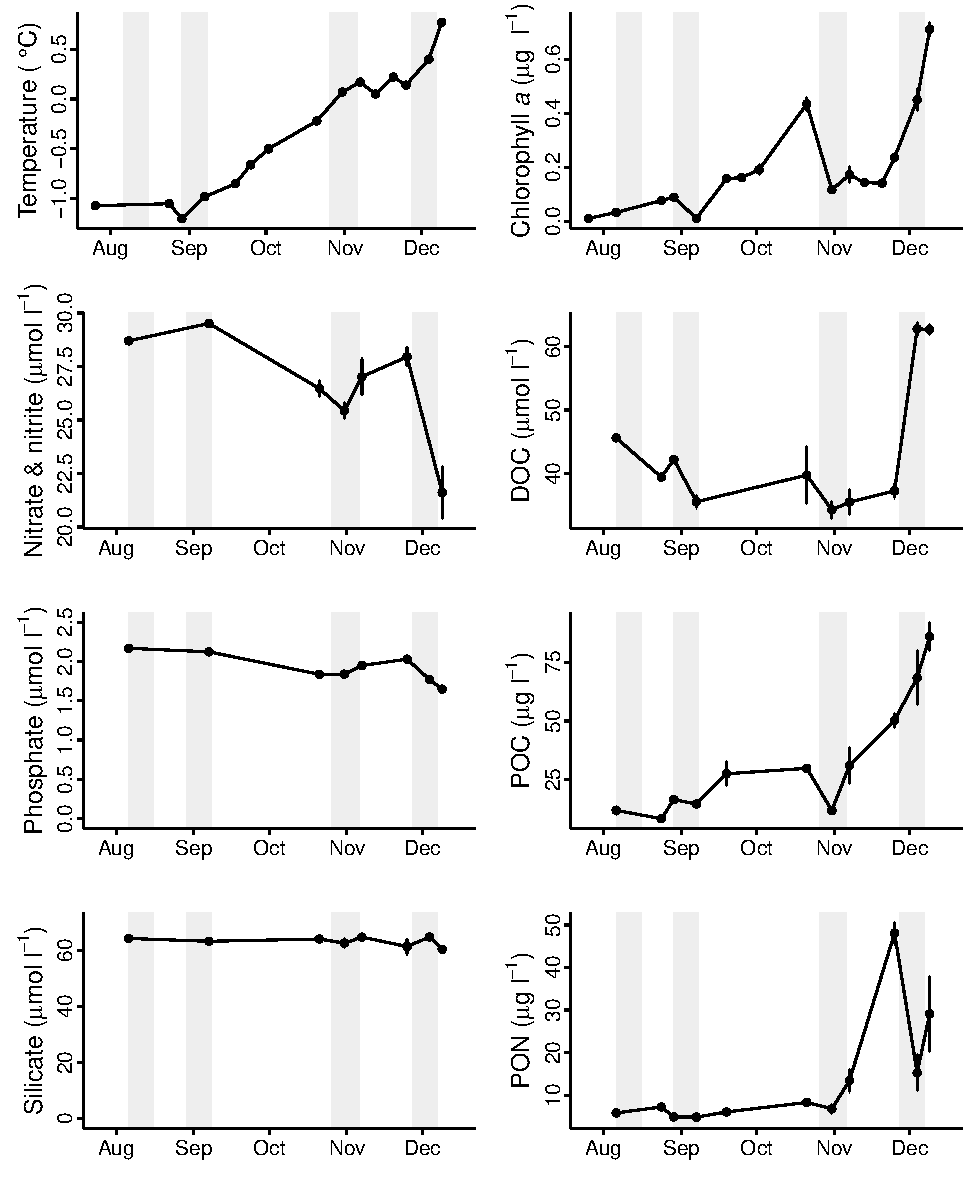
\includegraphics[width=0.8\textwidth]{Chapter_4_DOM/Figures/Supplemental_Figure_1_SWI_data}
\caption[Environmental conditions during the experimental period, August-December 2013.]{Temperature, inorganic nutrients (nitrate/nitrite, phosphate, silicate), chlorophyll \emph{a}, DOC, POC, and PON in the environment during the experimental period, August – December 2013. The timing of the four experiments is indicated by shaded bars.} 
\label{fig:ch3:swi} 
\end{figure}

\begin{figure}[ht!] 
\centering 
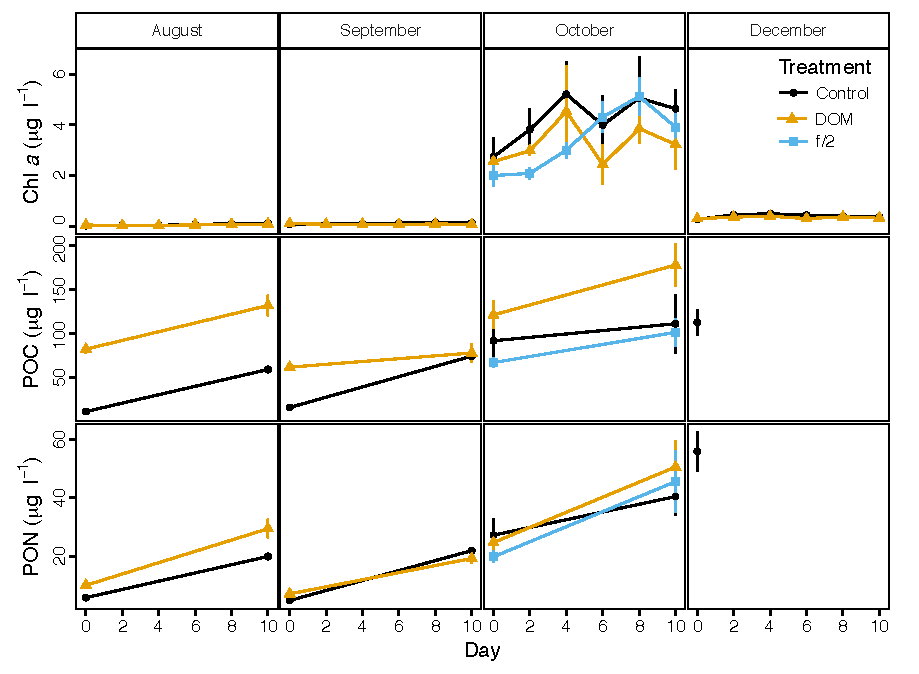
\includegraphics[width=\textwidth]{Chapter_4_DOM/Figures/Supplemental_Figure_2_Chla_POC_PON}
\caption[Chlorophyll \emph{a}, particulate organic carbon, and particulate organic nitrogen concentrations over the course of four experiments.]{Chlorophyll \emph{a}, particulate organic carbon, and particulate organic nitrogen concentrations over the course of four experiments.
} 
\label{fig:ch3:chla_poc_pon} 
\end{figure}

\begin{figure}[ht!] 
\centering 
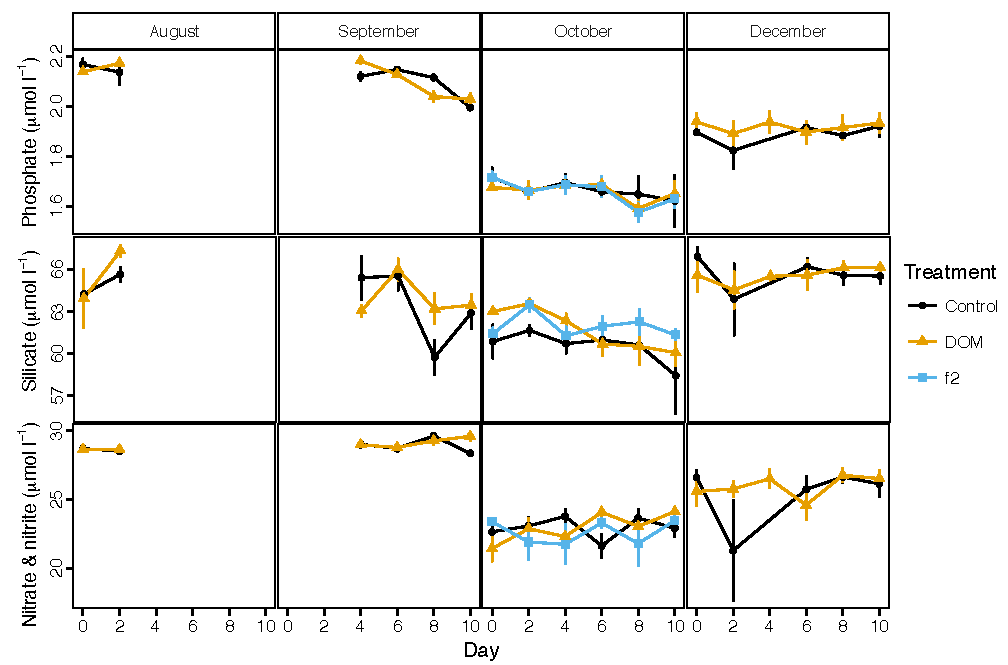
\includegraphics[width=\textwidth]{Chapter_4_DOM/Figures/Supplemental_Figure_3_Nutrients}
\caption[Inorganic nutrient (phosphate, silicate, and nitrate/nitrite) concentrations over the course of four experiments.]{Inorganic nutrient (phosphate, silicate, and nitrate/nitrite) concentrations over the course of four experiments.} 
\label{fig:ch3:nutrients} 
\end{figure}

\begin{figure}[ht!] 
\centering 
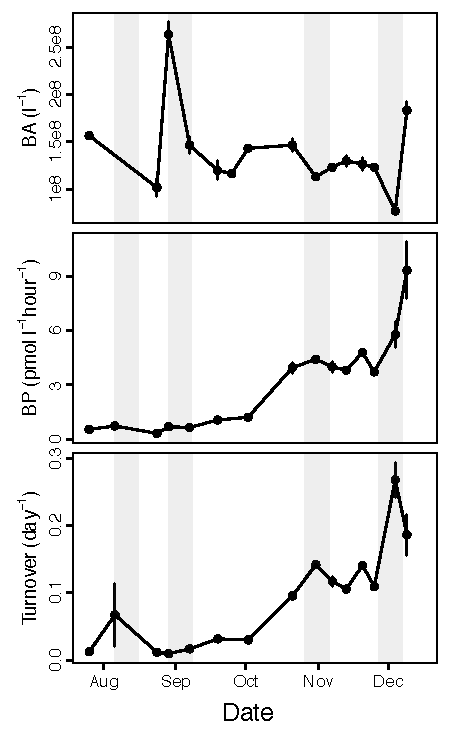
\includegraphics[width=0.5\textwidth]{Chapter_4_DOM/Figures/Figure_1_environment_BA_BP_turnover}
\caption[Bacterial abundance, bacterial production, and estimated community turnover rates in the environment during the experimental period, August – December 2013.]{Bacterial abundance (BA), bacterial production (BP), and estimated community turnover rates in the environment during the experimental period, August – December 2013. The timing of the four experiments is indicated by shaded bars.} 
\label{fig:ch3:environment_BA_BP_turnover} 
\end{figure}


Bacterial abundance increased over time in both control and DOM+ mesocosms, but the increases were more substantial in the DOM+ mesocosms than in the control mesocosms after Day 6 of the August, September, and October experiments (Figure \ref{fig:ch3:BA_BP_Turnover_Richness}). Although the initial values were similar, final DOM+ cell abundances were \textasciitilde{}50\% greater in October than in August and September. Treatment ($p = 0.0002$) and incubation day ($p = 6 \times 10^{-12}$) were more important drivers of variability than month ($p = 0.01$). Bacterial production (BP) increased over time in all mesocosms, but there were differences in BP between control and DOM+ mesocosms (Figure \ref{fig:ch3:BA_BP_Turnover_Richness}). During the first part of the season (August and September), BP increased more quickly in the DOM+ mesocosms, but BP in the control mesocosms ultimately reached similar levels, with 200- to 400-fold increases in all mesocosms. In the later part of the season (October and December) BP was fairly stable in the control mesocosms, with only 2- to 3-fold increases by Day 10. BP increased in the DOM+ mesocosms, but did not reach the same levels as earlier in the season, with only 10- to 20-fold increases. While BP varied between control and DOM+ mesocosms, treatment effects were less significant ($p < 0.005$) than the effects of day and month (both $p < 10^{-6}$). Estimated turnover rates tracked bacterial production, with the highest rates occurring in the DOM+ mesocosms in the August and September experiments.


\begin{figure}[ht!] 
\centering 
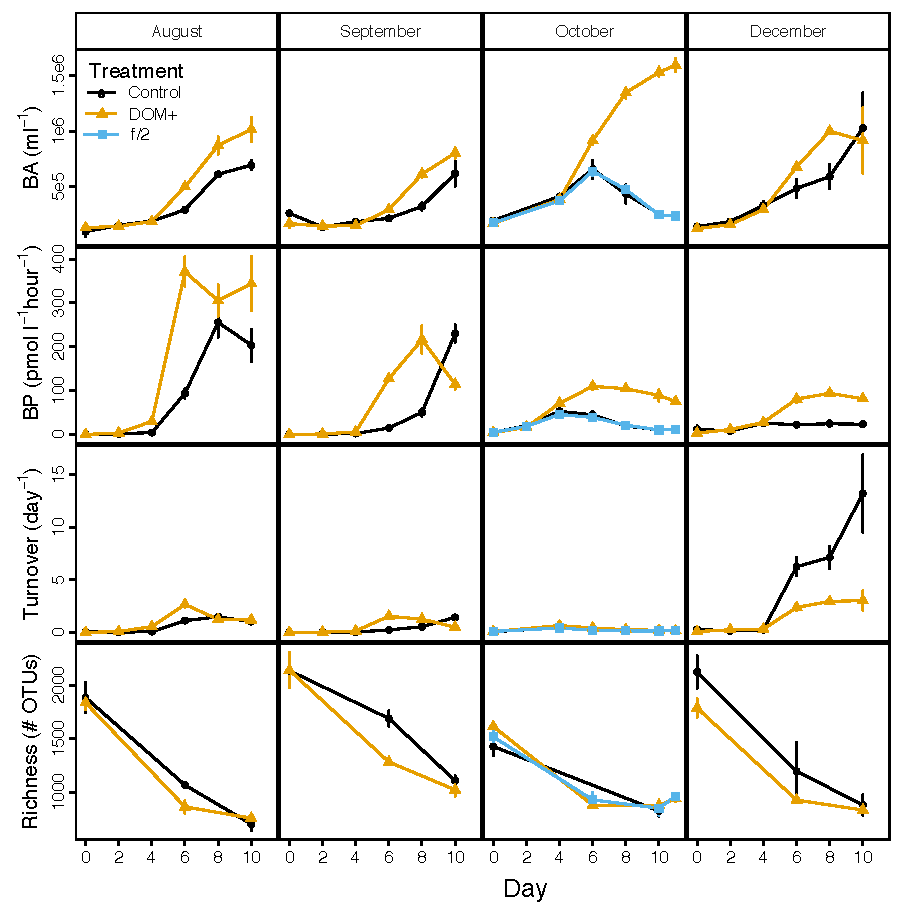
\includegraphics[width=0.9\textwidth]{Chapter_4_DOM/Figures/Figure_2_BA_BP_Turnover_Richness}
\caption[Bacterial abundance, bacterial production, estimated community turnover rates, and OTU richness over the course of four experiments.]{Bacterial abundance (BA), bacterial production (BP), estimated community turnover rates based on abundance and production, and observed OTU richness over the course of four experiments.} 
\label{fig:ch3:BA_BP_Turnover_Richness} 
\end{figure}


OTU richness, which was around 2000 OTUs on Day 0 of the August, September, and December experiments, had dropped to {\textless}1000 OTUs by Day 10 (Figure \ref{fig:ch3:BA_BP_Turnover_Richness}). Day 0 richness was slightly lower (\textasciitilde{}1500 OTUs) during the October experiment, but reached Day 10 levels similar to those in the other experiments. Evenness and Shannon diversity also declined in most mesocosms (Figure \ref{fig:ch3:alpha_diversity}). As with bacterial production, although the rate of decline sometimes varied between control and DOM+ mesocosms, day ($p < 2 \times 10^{-16}$) and month ($p < 10^{-6}$) outweighed treatment effects ($p < 0.1$). While OTU richness was significantly negatively correlated with both bacterial production ($p = 10^{-6}, r^{2}=0.25$) and abundance ($p < 3 \times 10^{-8}, r^{2}=0.35$), experimental day alone explained that greatest amount of variance ($r^{2}=0.71, p < 2 \times 10^{-16}$). 

\begin{figure}[htbp] 
\centering 
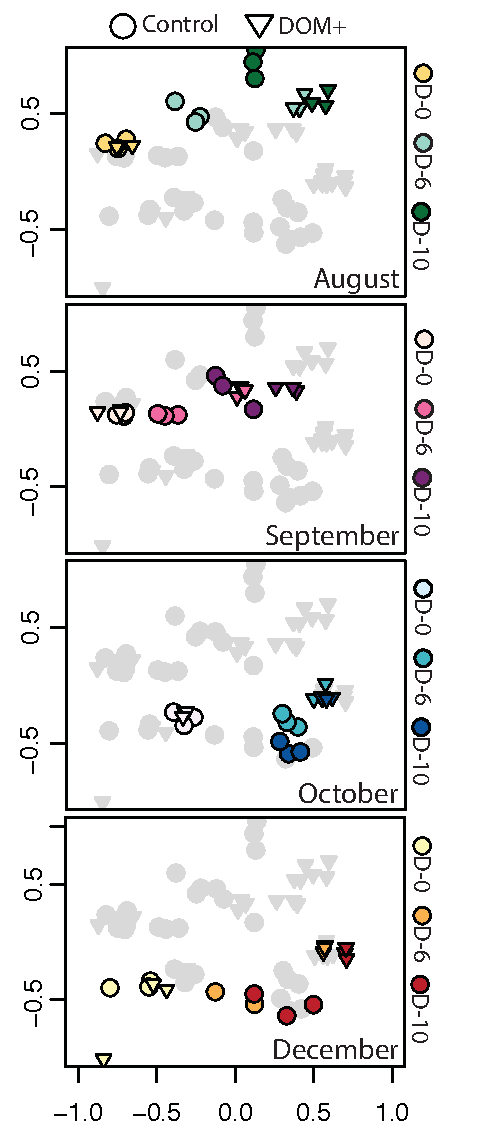
\includegraphics[width=0.5\textwidth]{Chapter_4_DOM/Figures/Figure_3_nmds}
\caption[Non-metric multidimensional scaling (NMDS) of Bray-Curtis similarity indices based on OTU relative abundance.]{Non-metric multidimensional scaling (NMDS) of Bray-Curtis similarity indices based on OTU relative abundance. Each point corresponds to an individual mesocosm replicate and sampling date ($n=3$ per time point per treatment). All samples from all experiments are shown in each panel. A different experiment is highlighted in each panel, with all other experiments shown in grey. Within each panel, different colors correspond to different sample days (0, 6, and 10). Control mesocosm communities are denoted by circles and DOM+ mescosm communities are denoted by triangles. For day 6 of the October experiment, f/2 control data is show in lieu of the regular control.} 
\label{fig:ch3:nmds} 
\end{figure}

\begin{figure}[ht!] 
\centering 
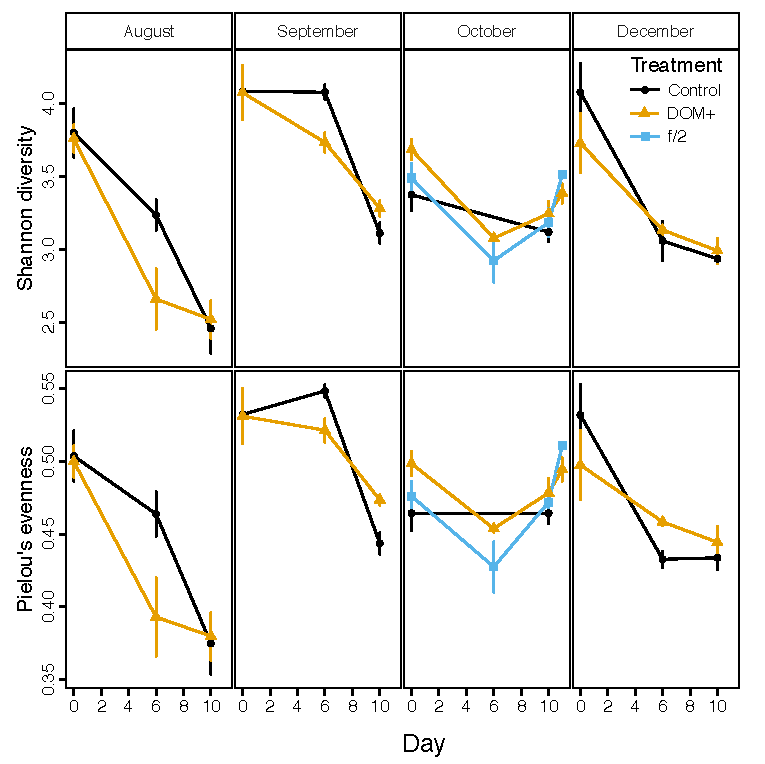
\includegraphics[width=\textwidth]{Chapter_4_DOM/Figures/Supplemental_Figure_4_alpha_diversity}
\caption[Alpha diversity metrics (Shannon diversity and Pielou’s evenness) over the course of four experiments.]{Alpha diversity metrics (Shannon diversity and Pielou’s evenness) over the course of four experiments.} 
\label{fig:ch3:alpha_diversity} 
\end{figure}

NMDS based on Bray-Curtis similarity visualizes how communities changed between months, experimental time points, and treatments (Figure \ref{fig:ch3:nmds}). NMDS axis 1 reflects changes that occurred within each experiment. By Day 6, the DOM+ mesocosm communities had reached or were quite close to their Day 10 state, while the control mesocosm communities continued to change as the experiment progressed. NMDS axis 2 reflects changes between experiments. The early spring experiments (August and September) and late spring experiments (October and December) are closely aligned with each other, but a relatively large shift occurred between September and October. Community composition in the first pair of experiments remained distinct from that in the second pair of experiments through the whole incubation period, indicating that the starting community composition was an important factor influencing the final community composition.


\begin{figure}[ht!] 
\centering 
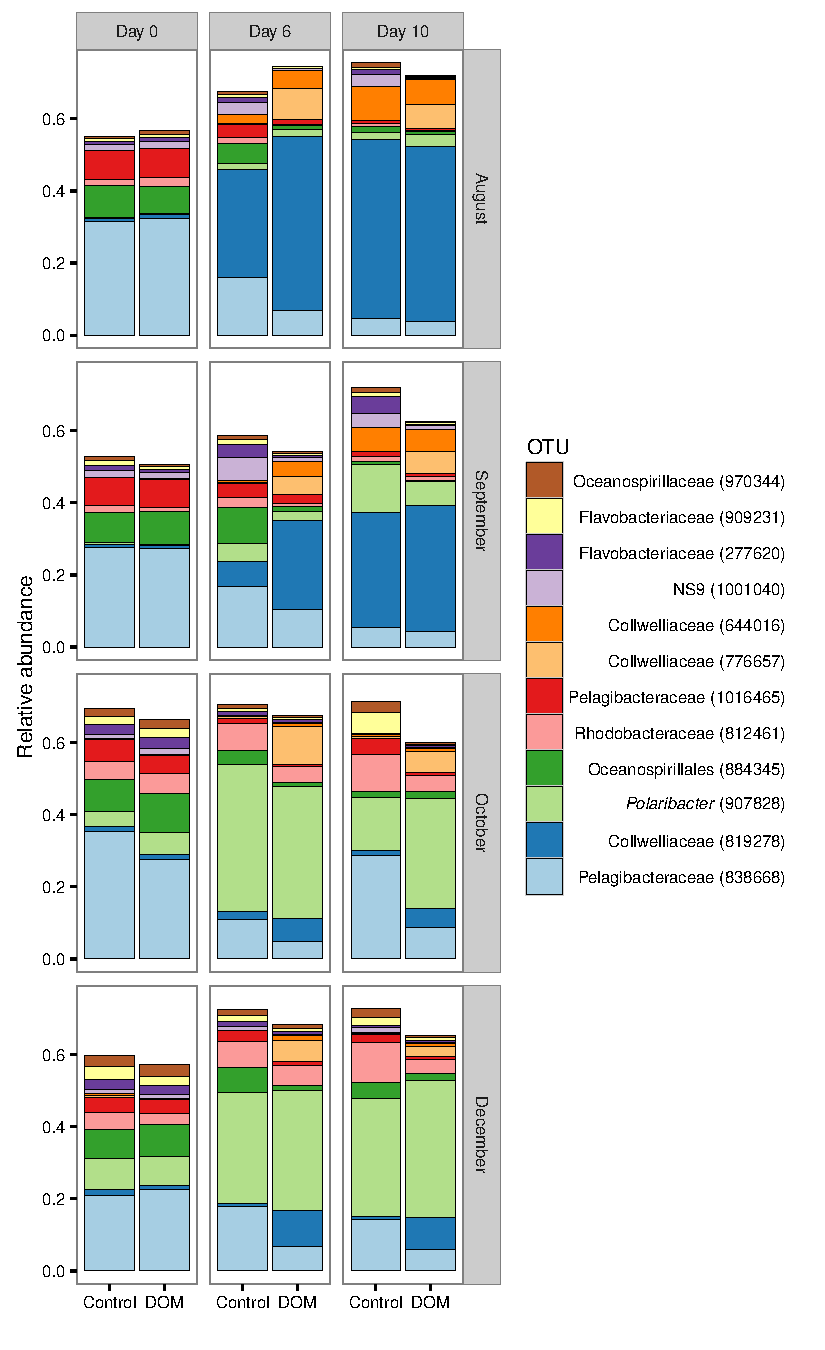
\includegraphics[width=0.8\textwidth]{Chapter_4_DOM/Figures/Figure_4_OTU_barplot}
\caption[Changes in the mean relative abundance of the top 12 OTUs (by mean relative abundance) across all experiments.]{Changes in the mean relative abundance of the top 12 OTUs (by mean relative abundance) across all samples. On Day 6 of the October experiment, the f/2 control is shown in lieu of the regular control.} 
\label{fig:ch3:otu_barplot} 
\end{figure}


Figure \ref{fig:ch3:otu_barplot}  shows the relative abundances of the top 12 OTUs (by mean relative abundance across all samples), which together represent ~50-75\% of each community. In all four experiments, OTUs classified as Pelagibacteraceae, Oceanospirillales, and SAR324 declined over time, while OTUs classified as Collwelliaceae and \emph{Polaribacter} increased in relative abundance. However, the relative importance of the two most abundant OTUs, Collwelliaceae (819278) and \emph{Polaribacter} (907828), shifted between September and October, with relatively small changes in initial community composition between September and October corresponding to much larger differences by the end of each experiment (Figure \ref{fig:ch3:otu_barplot}). In August and September, Collwelliaceae was slightly more abundant than \emph{Polaribacter} at Day 0. By Day 10, this difference was exaggerated with Collwelliaceae making up \textasciitilde{}40\% while \emph{Polaribacter} made up only \textasciitilde{}20\% of the community. As the season progressed, \emph{Polaribacter} became more prominent in the environment and the trend during experiments was reversed; by the end of the October and December experiments, Collwelliaceae made up only \textasciitilde{}7\% of the community, while Polaribacter made up \textasciitilde{}35\% of the community in DOM+ mesocosms. Of the top 12 OTUs, 6 varied in relative abundance by 5\% or more at one or more time points between the DOM+ and control communities (Figure \ref{fig:ch3:treatment_effect}). Colwelliaceae (819278 and 776657) were always more abundant in the DOM+ mesocosms, while Rhodobacteraceae (812461), Oceanospirillales (884345), and Pelagibacteraceae (838668) were always more abundant in the control. \emph{Polaribacter} (907828) displayed both positive and negative treatment effects at different times. 

\begin{figure}[htbp] 
\centering 
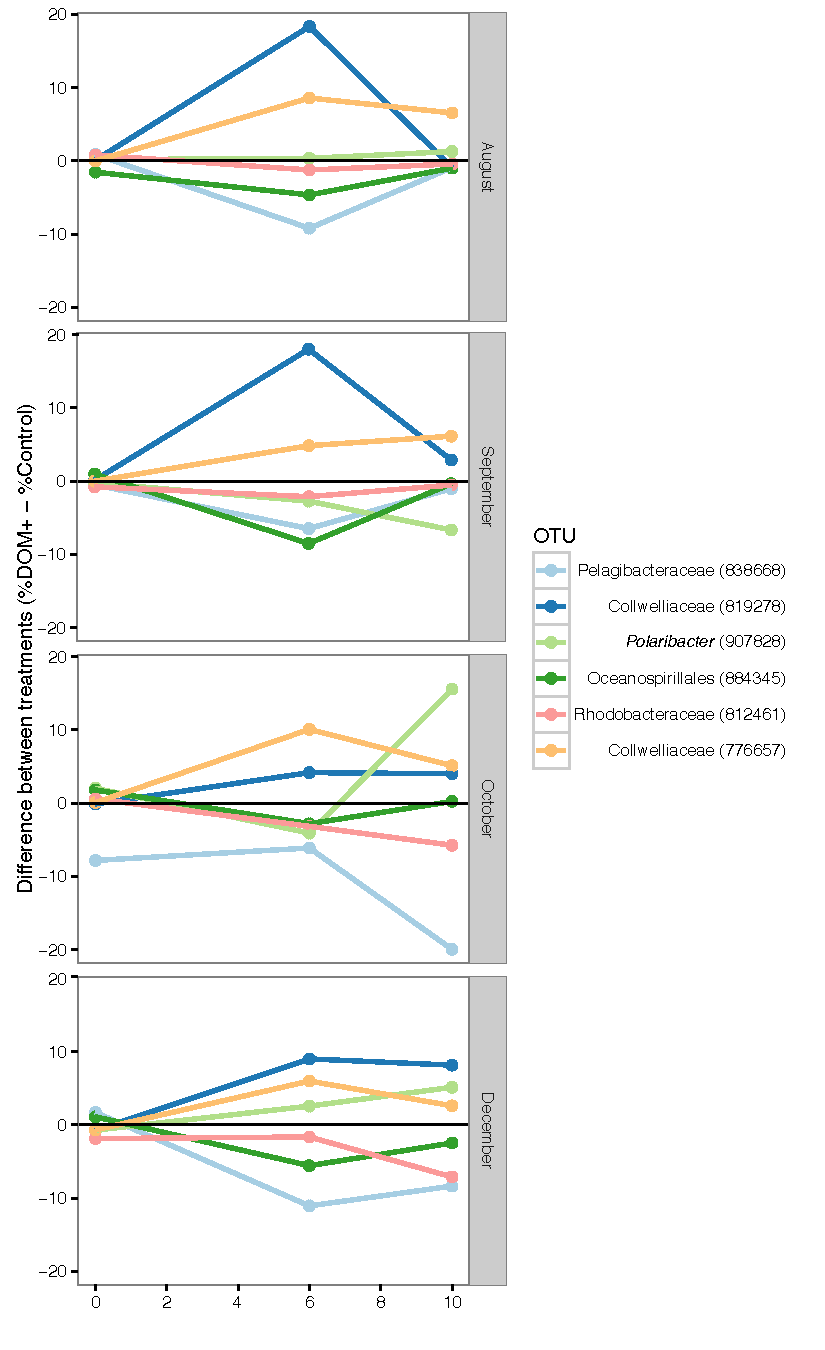
\includegraphics[width=0.8\textwidth]{Chapter_4_DOM/Figures/Figure_5_treatment_effect}
\caption[Difference in OTU relative abundance (\%) between the DOM-amended and control mesocosms.]{Difference in OTU relative abundance (\%) between the DOM-amended and control mesocosms. Out of top 12 OTUs (by mean relative abundance, see Figure 2), only OTUs showing more than ±5\% change are plotted. On Day 6 of the October experiment, the f/2 control is shown in lieu of the regular control.} 
\label{fig:ch3:treatment_effect} 
\end{figure}

We identified a sub-network of OTUs that were significantly associated with either the control group or the DOM treatment ($r > 0.5$; Figure \ref{fig:ch3:network}). All of the OTUs that were positively correlated with DOM+ were classified as Gammaproteobacteria, primarily Colwelliaceae. Several, but not all of these OTUs were negatively correlated with the control. Only one OTU, classified as NS9, was positively correlated with the control. A second sub-network linking OTUs to bacterial production shows that many Colwelliaceae OTUs correlated positively with bacterial production, as opposed to a number of Alphaproteobacteria OTUs, over half of them classified as Pelagibacteraceae, as well as two Gammaproteobacteria, HTCC2089 and HTCC2188, which were negatively correlated ($r > 0.7$).

\begin{figure}[htbp] 
\centering 
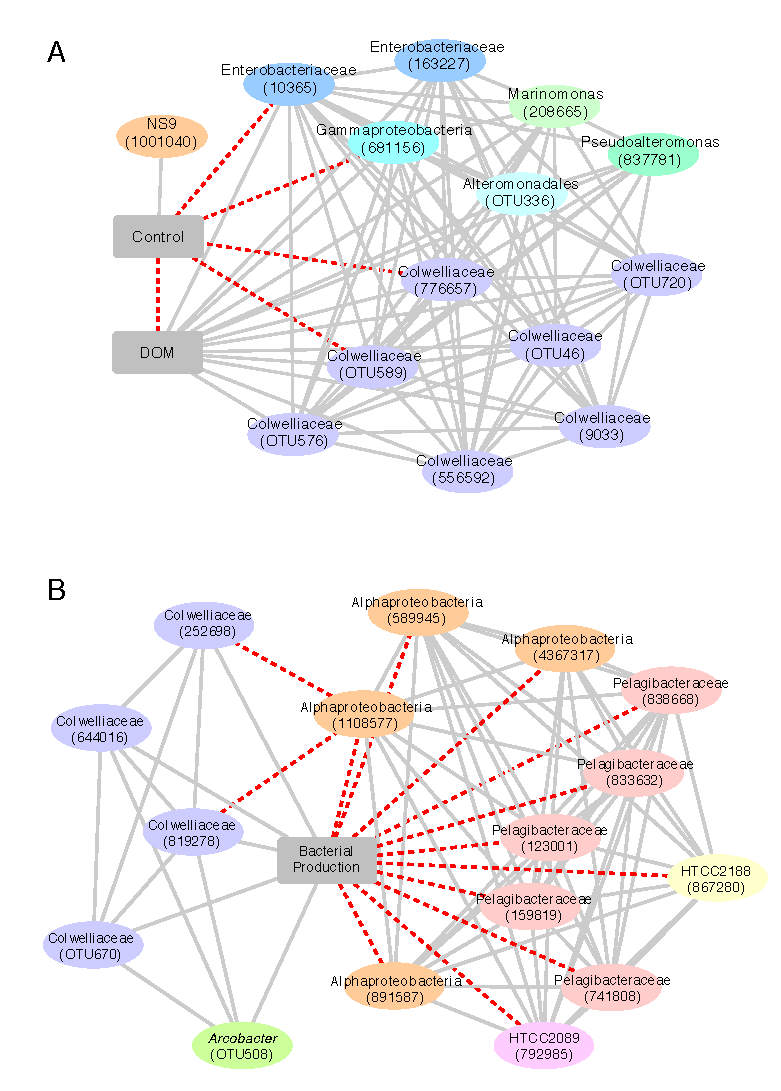
\includegraphics[width=0.9\textwidth]{Chapter_4_DOM/Figures/Figure_6_Network}
\caption[Sub-networks of highly correlated OTUs built around treatment level (control versus DOM+ and bacterial production.]{Sub-networks of highly correlated OTUs built around A) treatment level (control versus DOM+; $r > 0.5$) and B) bacterial production ($r > 0.7$). For clarity, only OTUs that appeared in at least 20\% of samples and had a mean relative abundance > $1$x$10^{-4}$ are shown. Solid, grey lines represent positive correlations; dashed, red lines represent negative correlations. Closest taxonomic identification and reference number (in parentheses) are given for each OTU.} 
\label{fig:ch3:network} 
\end{figure}

\section{Discussion}

Phytoplankton blooms and the resulting release of labile DOM are thought to be a major driver of marine bacterial community composition. Observational studies have shown that bacterial community composition and activity vary during phytoplankton blooms \citep{pinhassi2000seasonal,fandino2001variation,West2008-vp,tada2011differing,Teeling2012-jz,Klindworth2014-ba,wemheuer2015green}. This body of work suggests that bacterial succession allows for optimal DOM degradation, as bacterial groups with different metabolic strategies and substrate preferences display a high degree of niche partitioning in order to carry out different stages of DOM decomposition \citep{cottrell2000natural,alonso2007seasonal,poretsky2010transporter,rinta2012bacterial,sarmento2012use,Teeling2012-jz}. Niche partitioning may relieve direct competition between taxa and help explain high microbial diversity \citep{Teeling2012-jz,hutchinson1957concluding}. Alternatively, some studies have found that changes in DOM supply only slightly affect bacterial community composition, suggesting that physiological responses of metabolically versatile bacteria may be a factor, in addition to niche partitioning \citep{kirchman2004changes,rooney2005links,rink2007effects}.

There is growing evidence that labile organic matter availability is a primary factor controlling bacterial growth and community composition in Antarctica \citep{thingstad1991bacteria,Kirchman2009-sg,dsvse12,Kim2014-oj,luria2016seasonal}. However, directly testing the effects of phytoplankton-derived DOM on bacterial seasonal succession has proven challenging. Mesocosm experiments, like the one we conducted here, have traditionally relied on adding low molecular weight compounds like glucose or amino acids \citep{havskum2003silicate,allers2007response,gomez2012structuring}. For example, \citet{dmegm11} demonstrated that glucose enrichment of WAP seawater reduced bacterial diversity. Using more complex DOM substrates derived from phytoplankton cultures, several recent studies have shown that a wider range of bacteria respond readily to phytoplankton-, especially diatom-derived DOM, and that DOM originating from different phytoplankton species stimulates different bacterial phylogenetic groups \citep{sarmento2012use,nelson2012tracking,romera2011net}. Conversely, \citet{Landa2014-yg} and \citet{sharma2014distinct} found that varied natural DOM sources did not have differential effects on bacterial community composition despite variation in carbon quality and quantity. We selected the diatom \emph{T. weissflogii} as a DOM source as it is robust, well characterized, and a member of a genus that is widespread in the WAP region. However, the quantity and quality of DOM exuded by phytoplankton vary with species and physiological state and DOM from a single source (one species in one growth phase) does not represent the entire spectrum of changes in DOM composition and supply that probably occur during a phytoplankton bloom \citep{becker2014closely,Landa2014-yg}. 

Two OTUs were dominant across treatments, Colwelliaceae (819278) in the August and September experiments and \emph{Polaribacter} (907828) in the October and December experiments. Although marine Flavobacteria, including \emph{Polaribacter}, are heterotrophs that target high molecular weight organic matter and have been shown to increase in abundance during phytoplankton blooms, \emph{Polaribacter} did not show a consistent response to DOM amendments as opposed to simple `container effects,' the disturbance inherent in establishing a mesocosm \citep{cottrell2000natural,Pinhassi2004-kc,Abell2005-xu,gonzalez2008genome,Fernandez-Gomez2013-wr,Xing2015-kz,delong1993phylogenetic,Glockner1999-yc,West2008-vp,Teeling2012-jz}. The Colwelliceae family, on the other hand, responded quite strongly to DOM amendments, in excess of container effects. Colwelliaceae were abundant and diverse during the experiments, accounting for 9\% of all OTUs and 21\% of all sequences, as opposed to 3.6\% of OTUs and 2.6\% of sequences in the environment. A network of OTUs associated with DOM amendments was entirely comprised of Colwelliaceae and other Gammaproteobacteria. \emph{Colwellia} species are ubiquitous in polar environments and have been shown to metabolize an array of carbohydrates \citep{techtmann2016colwellia}. Interestingly, while Flavobacteria are perhaps more commonly associated with phytoplankton blooms, several previous studies have shown that Gammaproteobacteria, especially \emph{Alteromonas}, respond readily to natural DOM amendments during mesocosm experiments \citep{mccarren2010microbial,Landa2014-yg,romera2011net}.

Some of the changes in community structure observed during our experiments mirrored the changes that occur in the environment during a phytoplankton bloom. We compared abundant bacterial taxa from our mesocosm experiments to the seasonal time-series described in Chapter 3. Prevalent OTUs classified as Pelagibacteraceae (1016465 and 838668), Oceanospirillales (884345), and SAR324 (837879) decreased in both the experiment and the environment, while OTUs classified as \emph{Polaribacter} (907828), Flavobacteriaceae (1023473 and 909231), and Rhodobacteraceae (812461 and 789131) increased in both. Some of these changes presumably reflect resource partitioning to allow for optimal degradation. 

Although changes in the environment in substrate availability and bacterial community composition were relatively minor during the experimental period (August-December), as compared to the more dramatic changes that occurred during the January phytoplankton bloom, we observed substantial differences between experiments in bacterial production, turnover, and community composition. The maximum rate of bacterial production achieved in the DOM+ mesocosms halved between the September and October experiments. Furthermore, the shift between two dominant OTUs (i.e. \emph{Polaribacter} and Colwelliaceae) that occurred between the September and October experiments was striking. Relatively small changes in the abundances of these two OTUs in the environment were seemingly amplified during the experiments, resulting in divergent communities at the end of the early season experiments versus the late season experiments. 

The factors that governed this shift are unclear. Despite longstanding debate about the role of temperature in regulating bacterial production \citep{pomeroy2001temperature,Kirchman2009-sg}, a decade-scale study found that the relationship between bacterial production and temperature varied from year to year and was even negative in some years \citep{dsvse12}. Changes between experiments might also be attributable to differing bacterial mortality rates in the initial inoculum. Predation has been shown to increase exponentially with temperature and during natural and synthetic phytoplankton blooms \citep{garzio2013microzooplankton,Bird1991-sx,Duarte2005-dm}, while \citet{Brum2016-ig} found that viral abundance and lysogeny increased during the spring-to-summer transition. However, the extent to which initial mortality rates would have varied between experiments, when bacterial abundance and production were relatively stable in the environment, is unclear. 

Alternatively, we might attribute the observed changes not to concurrent environmental conditions but rather to historical contingencies \citep{martiny2006microbial}. Our initial hypotheses were grounded in the niche model of community assembly in which similar environmental conditions (e.g. DOM enrichment) select for the same or similar species from a diverse initial species pool, producing communities with similar structures \citep{fuhrman2006annually}. This contrasts with the neutral model of community assembly in which stochastic forces, including growth, dispersal, and mortality, dominate \citep{hubbell2001unified}. While the differences we observed may be governed by factors that we did not consider (i.e. predation), we suspect that stochastic `priority effects' played some role in determining the final community composition in our study. Disturbance events--in our case, enclosure in a container and DOM addition--have been shown to increase the relative importance of neutral processes in structuring communities and there is increasing evidence that dispersal, a largely stochastic process, has a more important role than previously thought \citep{telford2006dispersal,peay2010evidence,chytry2012dispersal,Fernandez-Gomez2013-wr}. 

A number of previous studies have reported divergent microbial community assembly in which inoculation of replicate environments with the same or similar initial communities results in different final community structures \citep{pagaling2014community}. \citet{langenheder2006structure} found that source communities collected from eight freshwater sites did not converge even when incubated under identical conditions for three weeks. Similar patterns of community assembly have been reported for desert hypolithic communities \citep{caruso2011stochastic}, wastewater treatment plants \citep{ofiteru2010pnas}, replicate laboratory biofilms \citep{Roeselers2006-tp}, and experimental wetlands \citep{baptista2008}. In some cases, these findings could be interpreted as priority effects in which random dispersal introduces variation in the initial relative abundance of species thereby altering final community structure despite the presence of environmental filtering \citep{nemergut2013patterns,chase2007drought,drake1990communities,fukami2011community}. Although priority effects have been demonstrated for sequential colonization of a site by microbes, the application of this concept to slight numerical advantages in a complex initial inoculum is less clear \citep{jiang2008community,peay2010evidence,warren2003mapping}. 

The apparent influence of priority effects on bacterial response to DOM in the WAP, where strong interannual and long-term climate change driven variation in sea ice extent and duration influences the timing and intensity of phytoplankton blooms, could have wider impacts on ecosystem function \citep{smith2008bellingshausen}. This study suggests that changes in bacterial community composition that take place before a phytoplankton bloom may set the stage for the influence of the phytoplankton bloom itself on the bacterial community. It follows, based on results of this study, that the trajectory of bacterial community succession may differ on an interannual basis in relation to the timing of phytoplankton blooms. It is not known whether historical filtering of bacterial communities, if it occurs, has broad ecological consequences, such as altering the fate of phytoplankton-derived carbon or interactive feedbacks on the growth of the phytoplankton community. 

\chapter{Seasonal and interannual variability in bacterial community composition in Antarctic coastal waters}\label{ch:lter}


\chapterdisclaimer{This work was performed in collaboration with Hugh Ducklow, Linda Amaral-Zettler, and Jeremy Rich.\\
\\
Hugh Ducklow and Linda Amaral-Zettler designed and conducted the study with Catherine Luria. Linda Amaral-Zettler and Jeremy Rich contributed sequence data. Catherine Luria analyzed data and wrote this report with guidance from Jeremy Rich. \\
\\
Data included in this chapter also appear in the following publication:\\
Bowman, J. S., Amaral-Zettler, L. A., Rich, J., Luria, C., and Ducklow, H. W. (2016). Bacterial community segmentation facilitates the prediction of ecosystem function along the coast of the western Antarctic Peninsula. \emph{ISMEJ} Accepted.
}


\section{Abstract}

The Western Antarctic Peninsula (WAP) is subject to strong seasonal variability driven by extreme fluctuations in daylength, interannual variability due to large-scale climatic drivers (e.g the Southern Annular Mode), and long-term variability due to rapid climate change in the region that has significantly increased temperatures and reduced sea ice cover over the last several decades. Despite important implications for the movement of materials and energy through the ecosystem, little is known about how these different scales of variability impact bacterial diversity and seasonal succession. Using 16S rRNA gene V6 hypervariable region amplicon sequencing, we assessed bacterial community composition across four Palmer LTER seasons, to identify patterns in seasonal variability and annually recurring successional patterns. While some of the broad trends that we observed were expected (e.g. a midsummer shift toward taxa that respond favorably to phytoplankton blooms), we also observed unexpected, isolated events (e.g. a Colwelliaceae bloom in December 2012) and a surprising degree of interannual variability. Bacterial communities by and large were comprised of a few ``persistent'' operational taxonomic units (OTUs) that were present in most or all samples throughout the time series, and thus, changes in community structures were largely driven by changes in the abundance of just a few taxa. These changes could be linked to both abiotic (day length, serial day, and macronutrients) and biotic (phytoplankton biomass and bacterial production and abundance) factors. Our four-year dataset demonstrates that bacterial community composition may be linked to phytoplankton dynamics, as well as underlying large-scale climatic forces.

\section{Introduction}

The WAP pelagic ecosystem is highly dynamic, with strong seasonal, interannual, and long-term variability. On a seasonal scale, the system oscillates between winters with almost continuous darkness and summers with over 20 hours per day of sunlight. Rapid changes in daylength during the spring transition period drive sea ice retreat and water column stratification. Shoaling of the upper mixed layer allows phytoplankton to overcome light limitation, allowing for intense phytoplankton blooms that support a highly productive food web \citep{Venables2013-me,Smetacek2005-tz}. Bacteria in turn modulate the movement of dissolved organic matter (DOM) produced during phytoplankton blooms through the system via the microbial loop and biological carbon pump \citep{Azam1991-xk,ducklow2001upper}. On an interannual scale, the WAP is subject to strong variability in physical and biological properties that has been linked to Southern Annular Mode (SAM) and El Nino-Southern Oscillation (ENSO) cycles \citep{saba2014winter,Kim2016-dl}. On a decadal scale, the WAP has responded dramatically to climate change; midwinter temperatures have increased by 6\textdegree C and sea ice extent has declined by 40\% over the past few decades \citep{dcddghmmmms12,Schofield2010-jj,Stammerjohn2008-nj}. 

Sea ice is a key driver of variability across multiple temporal scales as the annual advance, retreat and duration of sea ice strongly influence all aspects of the WAP ecosystem including the timing and magnitude of phytoplankton blooms \citep{dsvse12,mddfmss09}. Sea ice enhances primary production through increased water column stratification due to freshening of the surface water, enabling phytoplankton to persist and proliferate in the euphotic layer \citep{Smith1985-lx,Smith1986-en}. Conversely, in years of reduced sea ice, increased wind stress deepens the surface mixed layer, suppressing phytoplankton bloom formation \citep{saba2014winter}. 

Phytoplankton dynamics in turn influence WAP heterotrophic bacteria, which are thought to be primarily regulated by ``bottom up'' factors, particularly the availability of phytoplankton-produced labile DOM \citep{dsvse12,Kirchman2009-sg}. Bacterial production has been extensively studied in the region and is strongly linked to phytoplankton growth \citep{kim2016decedal,luria2016seasonal,dsvse12,Moran2001-ot}. However, there have been relatively few studies of the drivers of WAP bacterial community composition. Studies based on community fingerprinting techniques or on single winter and summer sampling dates report intense seasonality in bacterial and archaeal abundance, diversity, and metabolism \citep{Luria2014-dj,grwddecm12,mpmtbwd98,mg07}. \citet{Luria2014-dj} found similar bacterial communities in winter surface waters (10 m) and summer deep waters (100 m), habitats that share the common feature of reduced light and primary production. Significant changes in community composition concurrent with a summer phytoplankton bloom have also been reported for a single year \citep{luria2016seasonal}. These findings suggest that bacterial community composition responds to the availability of labile organic carbon from phytoplankton. However, the influence of interannual variability in climate modes and sea ice, and hence phytoplankton dynamics, on bacterial succession is unclear.

We surveyed community composition for free-living bacteria over the course of four Palmer Long Term Ecological Research (LTER) seasons (October-March, 2009-2013) and compared our findings to related Palmer LTER environmental datasets. Robust annual patterns have been reported in temperate systems including English Channel \citep{Gilbert2012-ta}, the mid-Atlantic Bight \citep{Nelson2008-fn}, and the coastal waters of Southern California \citep{chow2013temporal,fuhrman2006annually}, and rivers and lakes \citep{Crump2005-kv,Eiler2012-yh}, where temporal changes in community composition recurred on an annual basis with remarkable precision. In contrast, we hypothesized that, given the strong interannual variability in phytoplankton blooms, bacterial community composition would not exhibit strongly recurring annual patterns. Instead, changes in community composition would correspond to variable phytoplankton dynamics. 

\section{Methods}

\subsection{Contextual data collection}

Contextual data, including dissolved nutrients (phosphate, silicate, nitrate and nitrite), particulate organic carbon and nitrogen (POC and PON), chlorophyll \emph{a} (chl \emph{a}), primary production, bacterial abundance, and bacterial production, were collected through the Palmer LTER project. Protocols and curated data are available at \url{http://pal.lternet.edu/data}, as well as through the references cited below. Data from four years were analyzed: October 2009-January 2010 (PAL0910), December 2010-March 2011 (PAL1011), December 2011-March 2012 (PAL1112), and October 2012-March 2013 (PAL1213). Briefly, nutrient and DOC samples were filtered through combusted \SI{0.7}{\micro\meter} glass fiber filters (Whatman, GE Healthcare Life Sciences, Piscataway, NJ) and frozen at -80\textdegree C until analysis on a SEAL AutoAnalyer3 \citep{ducklow_doi_2016a} or Shimadzu TOC analyzer respectively \citep{ducklow_doi_2016c}. POC and PON samples were collected on combusted \SI{0.7}{\micro\meter} glass fiber filters from 0.5-2 L seawater and were frozen at -80\textdegree C until analysis via combustion \citep{ducklow_doi_2016d}. Chl \emph{a} samples, as with POC and PON, were collected on \SI{0.7}{\micro\meter} glass fiber filters from \textasciitilde{}0.5-2 L seawater and were assayed fluorometrically using acetone extracts \citep{schofield_doi_2016}. Primary production was derived from $^{14}$C uptake rates during incubation under in situ light conditions \citep{schofield_doi_2016a}. Bacterial abundance samples were analyzed by flow cytometry following the protocol of \citealt{Gasol2000-mn}, with SYBR\textsuperscript{\textregistered} Green I nucleic acid staining (Invitrogen, Carlsbad, CA) on an Accuri C6 flow cytometer (BD Biosciences, San Jose, CA) \citep{schofield_doi_2016}. Bacterial production was derived from rates of \ce{^3H}-leucine incorporation \citep{ducklow_doi_2016b}.

\subsection{16S rRNA gene library generation}

Samples were collected roughly once per week over the course of four LTER summer seasons using a Go-Flo bottle deployed to a depth of 0 m (2009-2010 and 2010-2011) or 10 m (2011-2012 and 2012-2013) at Arthur Harbor Station B (64\textdegree  46.80' S, 64\textdegree  4.45' W). Microbial communities were collected via vacuum filtration through successive 47-mm diameter \SI{3.0}{\micro\meter} pore-sized TSTP filters (EMD Millipore, Billerica, MA) and \SI{0.2}{\micro\meter} Sterivex{\texttrademark} cartridges (EMD Millipore, Billerica, MA). To preserve DNA, Sterivex cartridges were flooded with sucrose lysis buffer (40 mM EDTA, 50 mM Tris-HCl, 0.75 M sucrose) and were stored at -80\textdegree C until processing. We extracted DNA using a Puregene DNA extraction kit (Qiagen, Valencia, CA) with modifications as previously described \citep{amdh09} and stored extracts at -20\textdegree C until further processing. 

Sequence libraries were generated as in Chapter 3. For each DNA sample, the V6 hypervariable region of the 16S rRNA gene was amplified by polymerase chain reaction (PCR) with custom fusion primers that contained Illumina adaptor and inline barcodes (forward primer) or dedicated indices (reverse primer) as previously described \citep{Eren2013-ob}. Size-selected PCR products were quantified and pooled in equimolar amounts prior to sequencing on one lane of an Illumina HiSeq 1000 cycle paired-end run. 

\subsection{Data analysis}

Low-quality sequences were filtered from the resulting data by discarding reads without 100\% consensus between forward and reverse paired-end sequencing reads \citep{Eren2013-ob}. OTUs were clustered using Qiime (v 1.9.1; \citealt{Caporaso2010-ee}) with open reference OTU picking with the default UCLUST method \citep{Edgar2010-gq}, a minimum cluster size of 2, and a 97\% similarity threshold and were assigned Greengenes taxonomy (version 13\_8; \citealt{McDonald2012-qf}). After removing OTUs classified as chloroplasts, rarefied libraries were produced by randomly down-sampling to 40,000 sequences.

Richness calculations based on the number of OTUs observed in rarefied sequence libraries were compared with non-parametric Chao-Jost richness estimates based on un-rarefied libraries as implemented in the R package \code{iNEXT} \citep{Chao2012-nw, chao2014rarefaction}. Comparisons of observed richness between months (all years pooled) were made using one-way analysis of variance (ANOVA) followed by Tukey's HSD means comparisons using the \code{aov} and \code{TukeyHSD} commands in R \citep{t08}. We assessed the relationship between observed richness and environmental predictors, including serial day, daylength, phosphate, silicate, nitrate and nitrite, chlorophyll \emph{a}, and phaeopigment, using stepwise linear regression with forward-backward variable selection as implemented in the R packages \code{dynlm} and \code{MASS}, minimizing Akaike Information Criteria \citep{venables2002modern,zeileis2016dynlm}. Multivariate models were tested for multicollinearity among predictor variables using \code{vif} in the \code{car} package for R and models with variance inflation factors greater than 5 were discarded \citep{fox2011car}. 

We tested the top 100 OTUs, by mean relative abundance, for significant temporal trends or "seasonality" by fitting linear models, using the \code{lm} function in R, with serial day (days since October 31 within each LTER season) as the independent variable and logit-transformed relative abundance data as the dependent variable (c.f. \citealt{chow2013temporal}). We next divided samples (all years pooled) into either individual months or into two-month periods (October-November, December-January, and February-March) and identified those OTUs that best distinguished each category using a Random Forest supervised machine-learning algorithm as implemented in the R package \code{randomForest} \citep{Breiman2001-og,Liaw2002-zv}. The Random Forest consisted of 5000 classification trees with 77 OTUs evaluated at each node for all categories. 

To examine the relative effects of intra- and interannual variability, samples were grouped by month and by year and changes in community structure were analysed using permutational multivariate analysis of variance (PERMANOVA; \citep{McArdle2001-zn}). The analysis was based on mean group Bray-Curtis dissimilarity using Month and Year as factors and 999 permutations of residuals under a reduced model using \code{adonis}, after testing multivariate homogeneity of group dispersions using \code{betadisper} in the \code{vegan} package for R \citep{Oksanen_2015}. We also performed a Mantel test (Spearman, 999 permutations) comparing our Bray-Curtis dissimilarity matrix to a Euclidean distance matrix based on serial day (days since October 31) using the \code{mantel} function in \code{vegan} \citep{Oksanen_2015}. Beta diversity was visualized by non-metric multidimensional scaling (NMDS) using \code{metaMDS} also in the \code{vegan} package. 

We assessed relationships between environmental variables and OTU relative abundances using linear regression as described above. BIOENV analysis with Bray-Curtis dissimilarity and Spearman correlation \citep{Clarke1993-qq}, as implemented in \code{vegan}, was used to identify the environmental variables that best correlated with bacterial community similarities. Co-occurrence network analyses based on Pearson's correlations revealed relationships among OTUs and between OTUs and external variables (i.e. bacterial production). Networks were generated using the Cytoscape CoNet plugin version 1.1.1.beta and a subnetwork containing OTUs that correlated to bacterial abundance or production or chl \emph{a} ($r > 0.5$) was visualized in Cytoscape version 3.4.0   \citep{faust2012microbial,smobwr}.

All of our sequence data are MIMARKS-compliant \citep{Yilmaz:2011aa} and will be deposited in the NCBI SRA. Copies of the MIMARKS table and chapter figures as well as the R code used for all data analysis and figure production can be accessed at: \url{https://github.com/cmluria/dissertation/Chapter_5_LTER}. 

\section{Results and Discussion}

\subsection{Environmental variability}

The timing and magnitude of phytoplankton growth, based on primary production and chl \emph{a} (Figure \ref{fig:ch4:inorganic_nuts}), and bacterial responses (i.e. production and abundance; Figure \ref{fig:ch4:pp_chl}) varied from year to year. PAL0910 exhibited multiple chl \emph{a} peaks exceeding \SI{10}{\micro\gram \per\liter}, with the most sustained peak in late January coinciding with peaks in bacterial production and abundance. PAL1011 had moderate chl \emph{a} and a sustained period of high bacterial production. In contrast, PAL1112 had consistently low chl \emph{a} and primary and bacterial production. A prominent bloom ({\textgreater}\SI{30}{\micro\gram \per\liter} chl \emph{a}) occurred in early December during PAL1213, with a spike in bacterial production following two weeks later. When all years were pooled, log-log regression of bacterial production versus chl \emph{a} gave a slope of 0.55 ($r^{2} = 0.34$, $p < 0.001$). 

\begin{figure}[htbp] 
\centering 
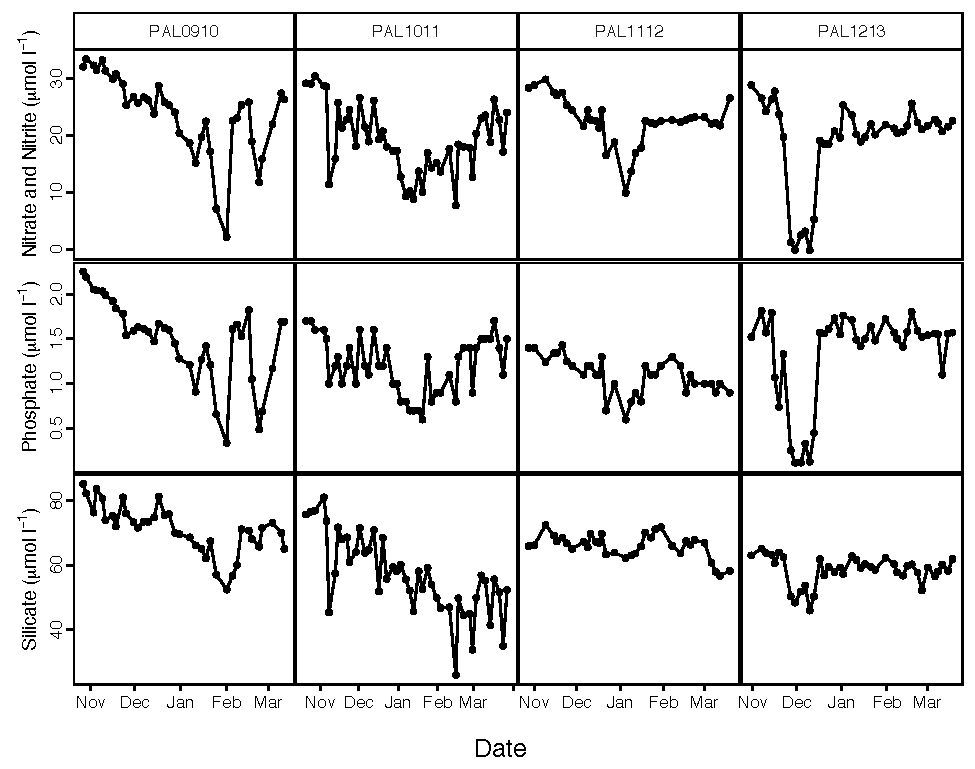
\includegraphics[width=1.0\textwidth]{Chapter_5_LTER/Figures/Figure_1_inorganic_nutrients}
\caption[Inorganic nutrients (nitrate and nitrite, phosphate, and silicate) at Station B across four LTER seasons (PAL0910-PAL1213).]{Inorganic nutrients (nitrate and nitrite, phosphate, and silicate) at Station B (0 m depth) in Arthur Harbor, for four LTER seasons (PAL0910-PAL1213)} 
\label{fig:ch4:inorganic_nuts} 
\end{figure}

\begin{figure}[htbp] 
\centering 
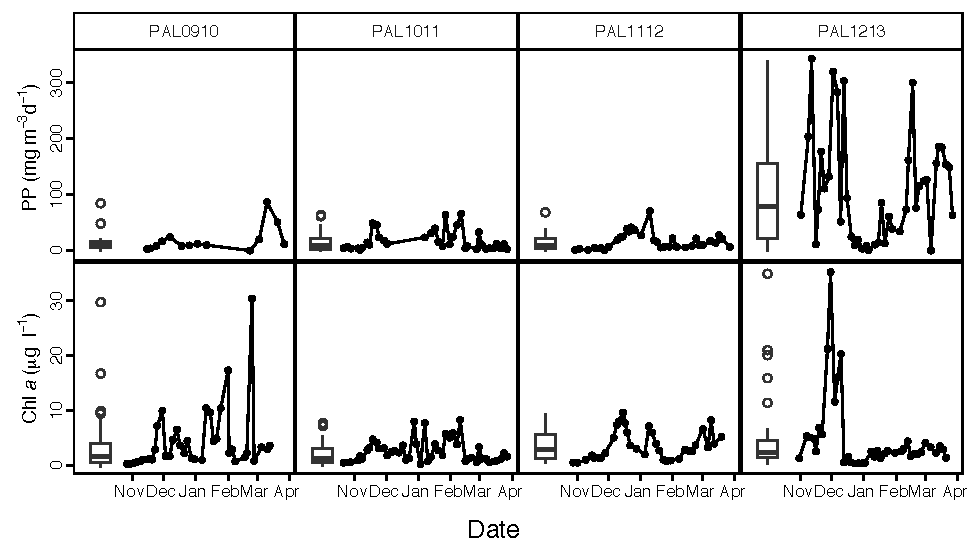
\includegraphics[width=1.0\textwidth]{Chapter_5_LTER/Figures/Figure_2_PP_Chl}
\caption[Phytoplankton dynamics (primary production and chl \emph{a}) at Station B  across four LTER seasons (PAL0910-PAL1213).]{Phytoplankton dynamics (primary production and chl \emph{a}) at Station B (0 m depth) in Arthur Harbor, for four LTER seasons (PAL0910-PAL1213).} 
\label{fig:ch4:pp_chl} 
\end{figure}

Inorganic nutrient drawdown corresponded to periods of increased chl \emph{a} (Figure \ref{fig:ch4:ba_bp}). Nitrate and nitrite and phosphate decreased substantially during the PAL0910 January and PAL1213 December blooms. Some silicate drawdown was evident at these times, as well as during the PAL1011 season when primary production and chl \emph{a} were relatively low. DOC generally oscillated between $45$ and \SI{60}{\micro\mole \per\liter} with no temporal trends evident (Figure \ref{fig:ch4:doc_poc_pon}). POC and PON peaked sharply after a chl \emph{a} peak in PAL0910 (Figure \ref{fig:ch4:doc_poc_pon}), but were surprisingly low during PAL1213, given the magnitude the PAL1213 December phytoplankton bloom. PON was relatively high during the period of sustained bacterial production and silicate drawdown in PAL1011. 

\begin{figure}[ht!] 
\centering 
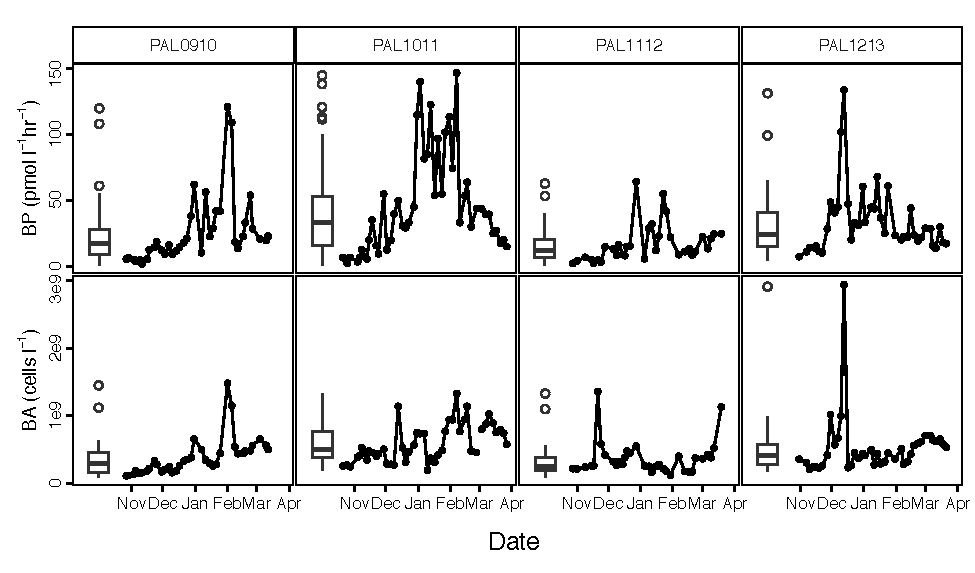
\includegraphics[width=1.0\textwidth]{Chapter_5_LTER/Figures/Figure_3_BA_BP}
\caption[Bacterial dynamics (production and abundance) at Station B across four LTER seasons (PAL0910-PAL1213).]{Bacterial dynamics (production and abundance) at Station B (0 m depth) in Arthur Harbor, for four LTER seasons (PAL0910-PAL1213)} 
\label{fig:ch4:ba_bp} 
\end{figure}

\begin{figure}[ht!] 
\centering 
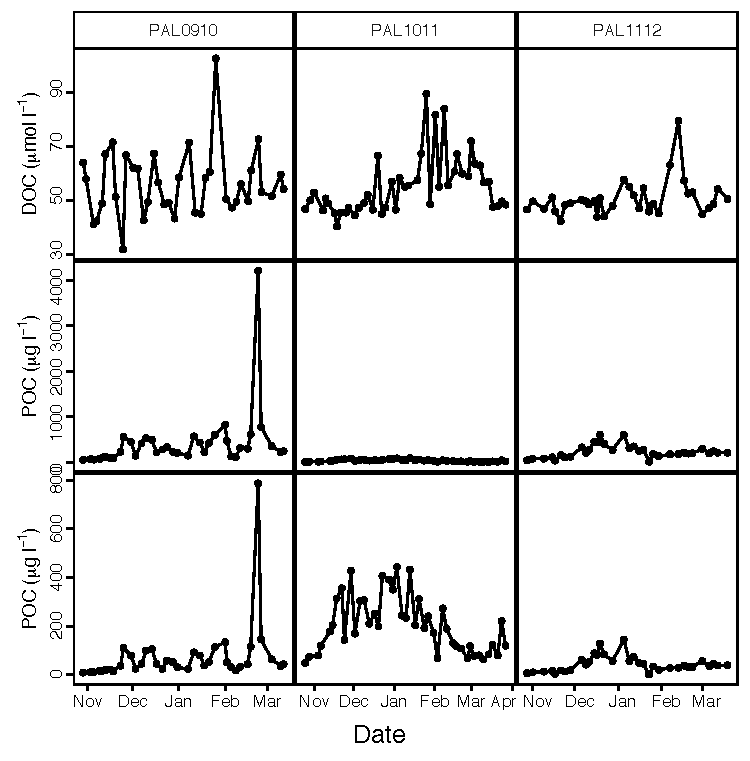
\includegraphics[width=1.0\textwidth]{Chapter_5_LTER/Figures/Figure_4_DOC_POC_PON}
\caption[Dissolved organic carbon and particulate organic carbon and nitrogen at Station B across three LTER seasons (PAL0910-PAL1112).]{Dissolved organic carbon (DOC) and particulate organic carbon (POC) and nitrogen (PON) at Station B (0 m depth) in Arthur Harbor, for three LTER seasons (PAL0910-PAL1112). Data from PAL1213 is not yet available.} 
\label{fig:ch4:doc_poc_pon} 
\end{figure}

The high levels of bacterial production, PON, and silicate drawdown for PAL1011 are surprising given the moderate levels of chl \emph{a} which we observed. This discrepancy was previously noted \citep{kim2016decedal}. \citet{saba2014winter}, pooling data from Station B and Station E and integrating chl \emph{a} and bacteria production for the top 50 m of the water column over almost 25 LTER seasons (PAL8788-PAL1112, December-February only), report a large, positive chl \emph{a} anomaly for PAL0910, a smaller positive anomaly for PAL1011 and a negative anomaly for the PAL1112 season. They attribute the positive anomalies to conditions favored under the negative phase of the SAM: increased winter ice extent and duration, reduced spring/summer winds, and increased water column stratification. Phytoplankton community composition during positive chl \emph{a} anomalies is generally dominated by diatoms, in accordance with the silicate drawdown we observed for PAL1011, whereas the relative abundance of cryptophytes increases in low chl \emph{a} years \citep{saba2014winter}.

\subsection{Persistence and seasonality of individual OTUs} 

Observed richness, or the number of OTUs present in rarefied libraries, varied between 349 and 876 OTUs, with a median of 585 (Figure \ref{fig:ch4:richness}). November had significantly greater richness than December, January, and March ($p < 0.05$) on average, but we did not observe robust seasonal trends, with midsummer richness minima, as previously reported for the WAP, as well as temperate systems \citep{luria2016seasonal,Ladau2013-ro,Gilbert2012-ta}. The lack of winter samples with presumably higher richness may have emphasized otherwise relatively minor fluctuations in richness between our summer samples. Chao-Jost estimated richness, based on un-rarefied libraries, ranged from 1098 to 4163 OTUs with a median of 2347 and was four times greater on average than observed richness based on rarefied libraries (Table \ref{table:ch5:richness}).


\begin{landscape}
\begin{table}[htbp]
\centering
\caption{Observed richness (number of OTUs) for rarefied sequence libraries and Chao-Jost estimated true OTU richness based on un-rarified sequence libraries with 95\% upper and lower confidence intervals (CI).}
\label{table:ch5:richness}
\tiny
\begin{tabular}{@{}lllll@{}}
\toprule
Sample Date & Observed Richness (Rarefied Libraries) & Estimated Richness (Un-rarefied Libraries) & Estimated richness 95\% Lower CI & Estimated richness 95\% Upper CI \\ \midrule
11/3/09     & 876                                    & 4163                                   & 3887                           & 4487                           \\
11/9/09     & 865                                    & 3719                                   & 3406                           & 4094                           \\
11/16/09    & 839                                    & 3423                                   & 3151                            & 3749                           \\
11/18/09    & 812                                    & 3729                                   & 3406                           & 4119                           \\
12/7/09     & 817                                    & 2716                                    & 2508                           & 2969                           \\
12/28/09    & 594                                    & 2846                                   & 2585                           & 3167                           \\
1/11/10     & 466                                    & 2007                                   & 1841                           & 2216                           \\
12/28/10    & 585                                    & 3413                                   & 3099                             & 3795                            \\
1/3/11      & 580                                    & 2547                                   & 2292                           & 2864                           \\
1/10/11     & 689                                    & 2671                                   & 2418                           & 2984                           \\
1/31/11     & 734                                    & 2402                                     & 2153                             & 2713                           \\
2/7/11      & 492                                    & 2590                                   & 2364                           & 2868                           \\
2/15/11     & 757                                    & 2594                                   & 2370                            & 2867                           \\
2/21/11     & 646                                    & 2756                                   & 2516                           & 3050                           \\
3/7/11      & 716                                    & 2781                                    & 2571                           & 3036                           \\
3/14/11     & 677                                    & 2807                                   & 2504                           & 3182                           \\
3/21/11     & 752                                    & 3792                                   & 3495                           & 4146                             \\
3/27/11     & 541                                    & 2873                                   & 2598                           & 3210                           \\
12/6/11     & 542                                    & 2308                                   & 2086                           & 2586                           \\
12/11/11    & 362                                    & 2175                                   & 1949                           & 2465                           \\
12/19/11    & 417                                    & 2176                                   & 1937                           & 2481                           \\
12/28/11    & 392                                    & 2427                                    & 2183                           & 2736                           \\
1/5/12      & 428                                    & 1884                                   & 1713                           & 2102                           \\
1/9/12      & 477                                    & 2503                                   & 2236                          & 2839                           \\
1/30/12     & 714                                    & 3083                                   & 2830                            & 3391                           \\
3/1/12      & 495                                    & 2167                                   & 1957                           & 2432                            \\
3/6/12      & 349                                    & 1329                                   & 1158                           & 1561                           \\
3/12/12     & 419                                    & 2215                                   & 1967                           & 2534                           \\
3/19/12     & 660                                    & 3219                                   & 2925                           & 3578                           \\
10/31/12    & 820                                    & 2904                                   & 2612                           & 3266                             \\
11/7/12     & 805                                    & 1865                                   & 1714                           & 2058                           \\
11/14/12    & 837                                    & 1889                                   & 1667                           & 2177                           \\
11/27/12    & 568                                    & 2015                                   & 1734                             & 2385                           \\
12/4/12     & 422                                    & 1412                                   & 1218                           & 1676                            \\
12/10/12    & 363                                    & 1687                                   & 1510                           & 1916                           \\
12/17/12    & 434                                    & 1394                                   & 1226                           & 1620                           \\
12/23/12    & 862                                    & 2727                                    & 2518                           & 2980                           \\
12/31/12    & 563                                    & 2347                                   & 2026                           & 2760                            \\
1/8/13      & 522                                    & 1672                                   & 1423                            & 2012                           \\
1/14/13     & 440                                    & 2272                                   & 1969                           & 2666                           \\
1/21/13     & 464                                    & 1098                                   & 980                            & 1257                           \\
1/31/13     & 660                                    & 1769                                   & 1569                           & 2028                           \\
2/12/13     & 393                                    & 1397                                   & 1249                           & 1594                           \\
2/18/13     & 665                                    & 1716                                   & 1507                           & 1991                           \\
3/6/13      & 427                                    & 1678                                   & 1492                           & 1922                           \\
3/11/13     & 612                                    & 1191                                    & 1045                           & 1389                           \\
3/18/13     & 843                                    & 1820                                   & 1615                           & 2084                           \\ \bottomrule
\end{tabular}
\end{table}
\end{landscape}

\begin{figure}[htbp] 
\centering 
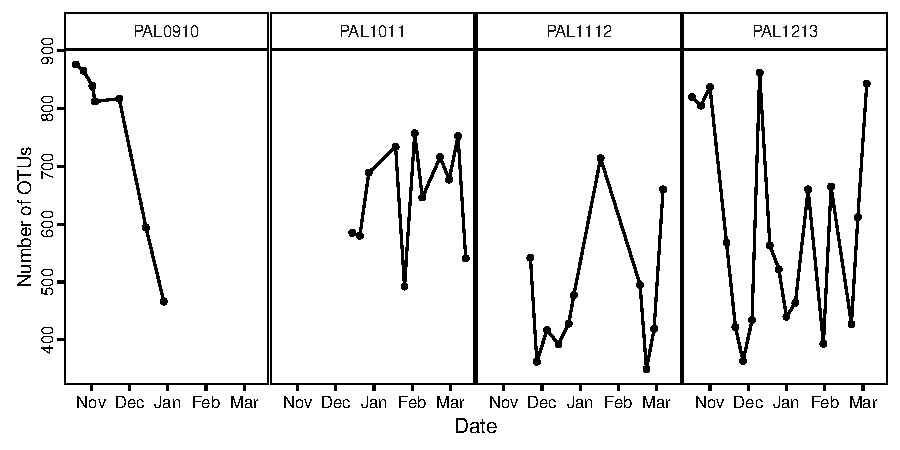
\includegraphics[width=1.0\textwidth]{Chapter_5_LTER/Figures/Figure_5_richness}
\caption[Bacterial OTU richness at Station B across four LTER seasons (PAL0910-PAL1213).]{Bacterial OTU richness at Station B in Arthur Harbor for four LTER seasons (PAL0910-PAL1213).} 
\label{fig:ch4:richness} 
\end{figure}

Throughout the time series, bacterial communities shared a common core structure. Of the 6143 total OTUs identified, 5482 were ``ephemeral'', appearing in less than 25\% of samples (Figure \ref{fig:ch4:persistence}). Only 144 were ``persistent'', present in more than 75\% of the samples; however, these OTUs accounted for 96.5\% of reads across samples. Fifty-three OTUs were found at every one of the 47 time-points, and these were exceptionally abundant in the sequence data, comprising 88\% of all reads. This pattern, in which a few persistent taxa are also consistently abundant, suggests that many of the changes we observed in community composition reflect variations in the relative abundance of these persistent taxa, as opposed to extinction and colonization processes \citep{Caporaso2011-ec}. Similar findings, in which a few persistent OTUs are also the most abundant, have been reported for the Western English Channel, station ALOHA, California coastal waters, and a freshwater lake \citep{Eiler2011-jl,Eiler2012-yh,Gilbert2009-yi,Caporaso2011-ec,chow2013temporal}. 

\begin{figure}[ht!] 
\centering 
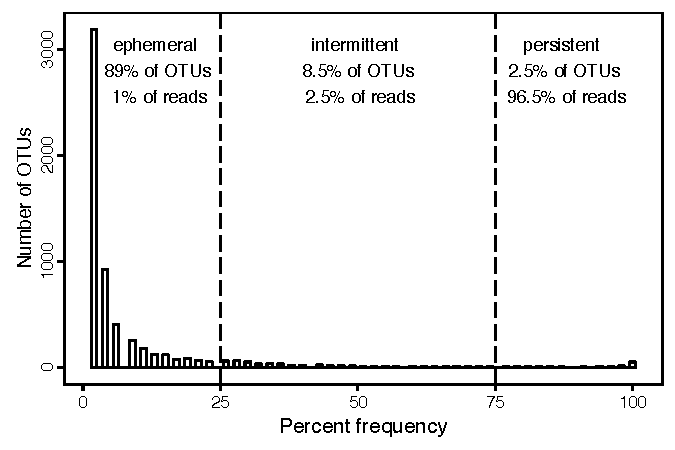
\includegraphics[width=1.0\textwidth]{Chapter_5_LTER/Figures/Figure_6_OTU_persistence}
\caption[Distribution of ``ephemeral'', ``intermittent'', and ``persistent'' OTUs.]{Number of OTUs that occur at different frequencies. Percent frequency was defined as the number of timepoints out of the total timepoints sampled (n=47) that an OTU appeared. OTUs that appeared at less than 25\%, in 25-75\%, or in more than 75\% of the total timepoints were respectively labeled as ``ephemeral'', ``intermittent'', and ``persistent''.} 
\label{fig:ch4:persistence} 
\end{figure}

Forty-three of the top 100 OTUs displayed ``seasonality'', based on a significant correlation with serial day or days since October 31 (all years pooled; $p < 0.05$). These seasonal OTUs accounted for \textasciitilde{}40\% of the community on average. The ten most abundant (by mean relative abundance) of these seasonal OTUs are shown in Figure \ref{fig:ch4:seasonal_otu}. Most but not all OTUs followed a somewhat consistent trajectory; for example, \emph{Polaribacter} (907828) always peaked during the first half of the season, while Flavobacteriaceae (1023473) always declined as the season progressed. 

\begin{figure}[htbp] 
\centering 
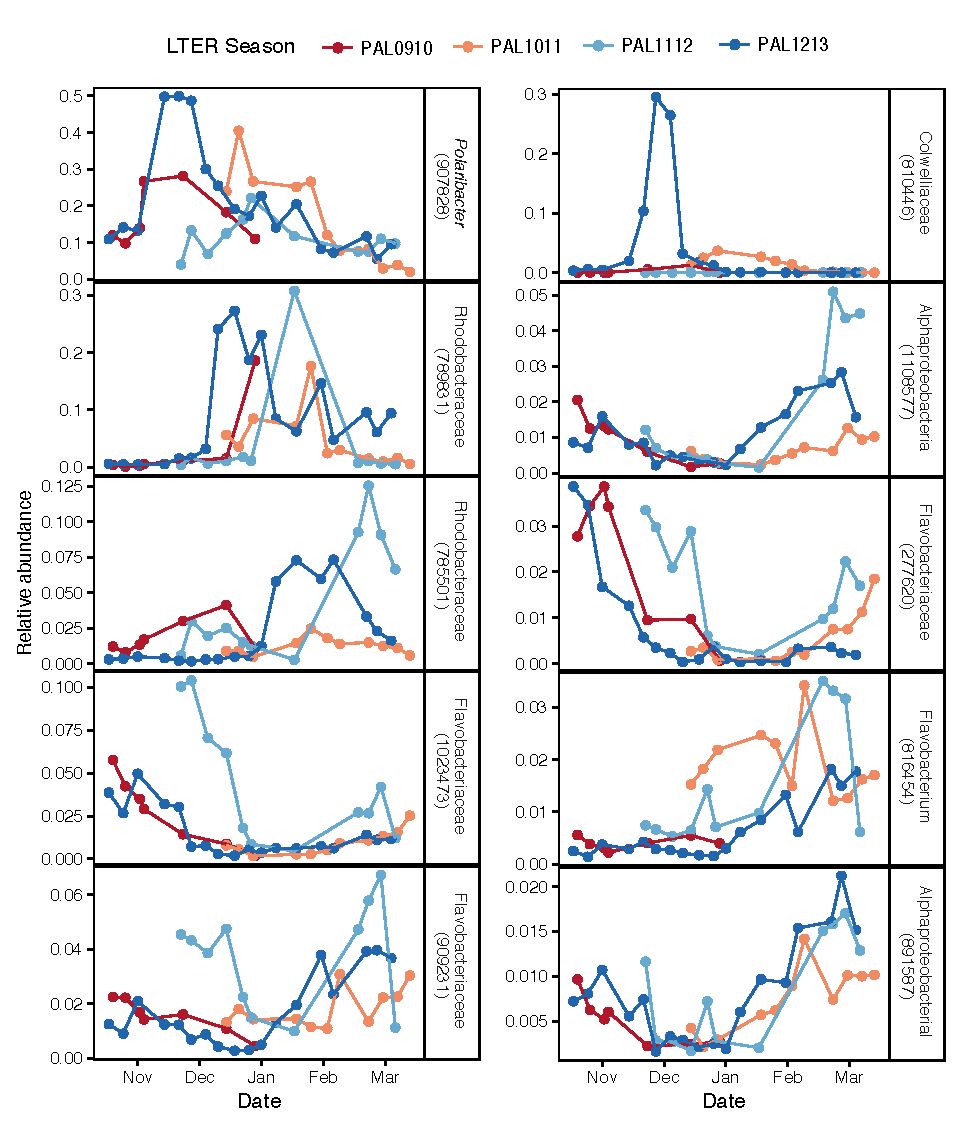
\includegraphics[width=1.0\textwidth]{Chapter_5_LTER/Figures/Figure_7_seasonal_otus}
\caption[Ten most abundant OTUs that displayed ``seasonality''.]{Ten most abundant OTUs (based on average relative abundance) that displayed ``seasonality'', with a significant correlation ($p < 0.05$) between relative abundance and serial day (days since October 31 for each season).} 
\label{fig:ch4:seasonal_otu} 
\end{figure}

\subsection{Seasonal and annual trends in overall community composition}

In general, we did not observe the same sort of robust, recurring annual patterns reported in other marine systems \citep{Gilbert2012-ta,Nelson2008-fn,chow2013temporal,fuhrman2006annually}. Using discriminant function analysis (DFA) to search the taxa that were best able to predict month, \citet{fuhrman2006annually} and \citet{Gilbert2012-ta} were able to assign 80-100\% of samples to the correct month based solely on the distribution and abundance of OTUs, demonstrating interannual repeatability. Similarly, we used Random Forest analysis, a machine learning method of classification, to categorize samples either by individual month or by two-month period (all years pooled): October/November (spring), December/January (mid-summer), and February/March (late summer/early autumn). Unlike DFA, Random Forest analysis does not have any assumptions about the underlying distribution of data and can create models that capture nonlinearities and higher order interactions \citep{Breiman2001-og}. With samples pooled by individual month, Random Forest analysis categorized samples with a 35\% ``out of bag'' error rate. Dividing samples into three two-month categories improved the model, reducing the error rate to 11\%. This suggests that while some repetition in community structure occurs from year to year in the WAP, the patterns are less precise than those reported for other systems. Table \ref{ch4:tab:rf_top} shows the top 20 most predictive OTUs for each two-month period. Some of the predictive OTUs were relatively abundant (e.g. \emph{Polaribacter}), while others were relatively rare but nonetheless predictive of a given time period. Many of the same OTUs were identified as predictive for both the December-January and February-March time periods, while all but one of the OTUs identified for October-November were unique to that category.

\afterpage{
\begin{landscape}
\begin{table}[htbp]
\centering
\caption[Results from Random Forest analysis, identifying OTUs that are predictive of different temporal periods across multiple years.]{Random Forest analysis results. Top 20 predictive OTUs and their nearest taxonomic affiliation for each of three two-month periods (all years pooled): October/November, December/January and February/March.}
\label{ch4:tab:rf_top}
\footnotesize
\begin{tabular}{@{}llllll@{}}
\toprule
\multicolumn{2}{c}{October/November}      & \multicolumn{2}{c}{December/January}        & \multicolumn{2}{c}{February/March}            \\ \midrule
1057746             & Alphaproteobacteria & 1108577             & Alphaproteobacteria   & 1108577             & Alphaproteobacteria     \\
145979              & Acidimicrobiales    & 1110047             & Alteromonadaceae      & 1110047             & Alteromonadaceae        \\
146541              & Cryomorphaceae      & 171966              & Flavobacteriales      & 234515              & Flavobacteriales        \\
158564              & Arctic97B-4         & 234515              & Flavobacteriales      & 3549277             & Rhodobacteraceae        \\
2287192             & Rhizobiales         & 251424              & Rhodobacteraceae      & 3751007             & Flavobacteriales        \\
3223711             & Alphaproteobacteria & 3223711             & Alphaproteobacteria   & 4296166             & \textit{Sediminicola}   \\
339872              & Rhodobacteraceae    & 3751007             & Flavobacteriales      & 541534              & Flavobacteriaceae       \\
4411525             & Rhodospirillaceae   & 396244              & Cryomorphaceae        & 590937              & Rhodobacteraceae        \\
553079              & \textit{Nitrospina} & 4296166             & \textit{Sediminicola} & 594314              & Chromatiales            \\
562219              & Rhodospirillaceae   & 590937              & Rhodobacteraceae      & 741808              & Pelagibacteraceae       \\
567397              & Rhodospirillaceae   & 591094              & Candidatus Portiera   & 752629              & ZD0117                  \\
594314              & Chromatiales        & 752629              & ZD0117                & 792985              & HTCC2089                \\
639731              & \textit{Rubritalea} & 786176              & Rhodobacteraceae      & 816454              & \textit{Flavobacterium} \\
789831              & Rhodobacteraceae    & 792985              & HTCC2089              & 823476              & Alteromonadaceae        \\
830414              & Rhodobacteraceae    & 835045              & Rhodobacteraceae      & 835045              & Rhodobacteraceae        \\
833561              & Pelagibacteraceae   & 891587              & Alphaproteobacteria   & 891587              & Alphaproteobacteria     \\
921366              & \textit{Nitrospina} & 907828              & \textit{Polaribacter} & 907828              & \textit{Polaribacter}   \\
936371              & \textit{Nitrospina} & New.ReferenceOTU481 & Pelagibacteraceae     & New.ReferenceOTU481 & Pelagibacteraceae       \\
New.ReferenceOTU498 & Alphaproteobacteria & New.ReferenceOTU495 & Colwelliaceae         & New.ReferenceOTU495 & Colwelliaceae           \\
New.ReferenceOTU763 & Rhodospirillaceae   & New.ReferenceOTU725 & Unassigned            & New.ReferenceOTU725 & Unassigned              \\ \bottomrule
\end{tabular}
\end{table}
\end{landscape}
}

We also considered how overall community composition varied across different temporal scales. A Mantel test comparing community dissimilarity (Bray-Curtis) and serial day (Euclidean) distance matrices found a statistically significant, but weak relationship between community composition and elapsed time ($r = 0.26$, $p = 0.001$). A PERMANOVA comparison of mean group Bray-Curtis dissimilarities showed that community composition in the months of November ($r = 0.29$), December ($r = 0.67$), January ($r = 0.48$), and March ($r = 0.63$) varied significantly between years (all $p < 0.05$) with the greatest differences observed for December and March. It should be noted that we also observed significant variance in group dispersion among December samples, which violates the implicit assumption of roughly constant within-group multivariate dispersion and could have contributed to the significant PERMANOVA result for that month. Taken together, these results indicate that community composition for a given day or month varies from year to year.

Non-metric multidimensional scaling suggests that while bacterial succession is somewhat predictable from year to year, interannual variability is substantial. (Figure \ref{fig:ch4:nmds}). Some grouping by month across multiple years is evident along NMDS axis 2, indicating a degree of interannual repetition. Spring/early summer (October and November) samples are relatively close to each other, while mid-summer (December, January, and February) samples are more widely scattered. Late summer (March) samples fall at an intermediate point between the two other groups. Some clustering of samples by year is also apparent, especially for PAL1011 and PAL1112, along NMDS axis 1. 

\begin{figure}[htbp] 
\centering 
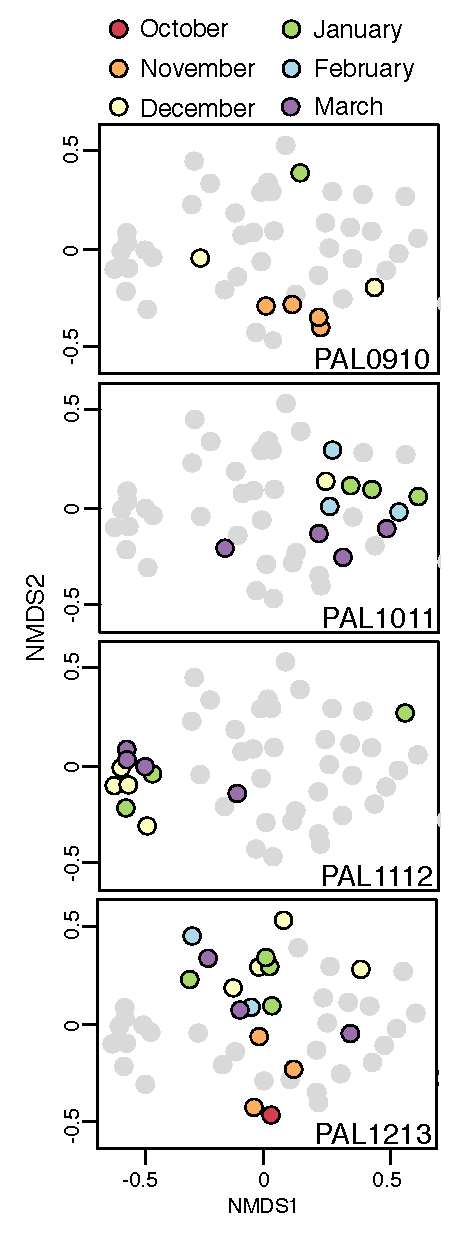
\includegraphics[width=0.5\textwidth]{Chapter_5_LTER/Figures/Figure_8_NMDS}
\caption[Non-metric multidimensional scaling of Bray-Curtis similarity indices based OTU relative abundance.]{Non-metric multidimensional scaling of Bray-Curtis similarity indices of bacterial community composition based OTU relative abundance. A different Palmer LTER season is highlighted in each panel with samples from seasons that are not highlighted shown in grey. Stress = 0.20.} 
\label{fig:ch4:nmds} 
\end{figure}


Finally, we compared pairwise Bray-Curtis similarity versus time elapsed between samples in months (Figure \ref{fig:ch4:bray_curtis}). \citet{chow2013temporal} performed a similar analysis showing annual recurrence as evidenced by Bray-Curtis similarity maxima every 12 months and a slight but significant erosion of community similarity over the course of a decade. We did not observe a similar cyclical pattern in our dataset, nor a significant long term trend. Samples collected even 3 months apart were more similar on average than samples collected exactly 12 months apart, providing little evidence of a repeated annual cycle. However, it is important to note that our time series only spanned the October-March period and did not include the austral winter. Therefore, even ``opposite'' samples, i.e. samples separated by six months, would have been collected in the spring and fall, when communities are relatively similar. The addition of winter samples to our time series would presumably decrease Bray-Curtis similarity between samples collected 6, 18, and 30 months apart and the Bray-Curtis similarity between samples collected exactly 12 months apart would be greater by comparison, perhaps revealing a cyclical pattern. 

\begin{figure}[htbp] 
\centering 
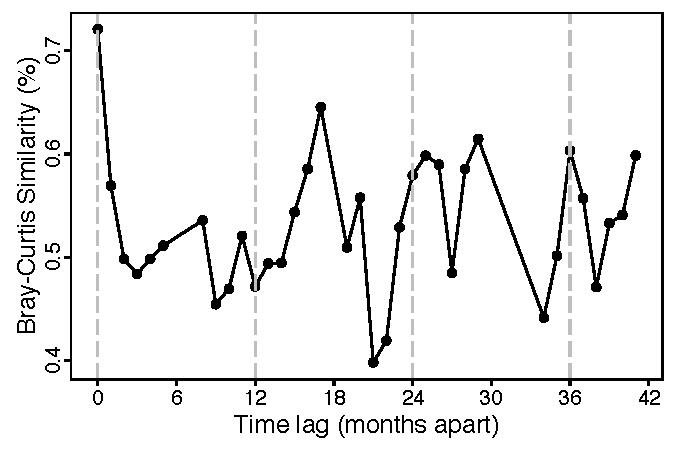
\includegraphics[width=0.8\textwidth]{Chapter_5_LTER/Figures/Figure_9_bray_curtis_over_time}
\caption[Mean pairwise Bray-Curtis community similarity over elapsed time.]{Seasonal and interannual patterns in Bray-Curtis community similarity. Average pairwise community similarity is shown on the Y-axis while the X-axis indicates time lag, the number of months between the communities compared.} 
\label{fig:ch4:bray_curtis} 
\end{figure}

\subsection{Coupling Bacterial Community Structure with Environmental Changes}

Some broad trends in taxonomic succession emerged over the course of several seasons that can be attributed to environmental changes. Among the more prevalent taxa, Pelagibacteraceae, Oceanospirillales, NS9, Rhodospirillales, SAR324, SAR406, and \emph{Nitrospina} tended toward lower relative abundance at mid-summer, while Flavobacteriales, including \emph{Polaribacter} and Rhodobacteraceae, tended toward greater relative abundance at mid-summer (Figure \ref{fig:ch4:taxa} ). The relatively high abundance of SAR406, \emph{Nitrospina}, and SAR324 earlier in the season reflects previous suggestions that chemolithoautotrophy is an important component of bacterial metabolism during the winter \citep{grwddecm12,williams2012metaproteomic,manganelli2009major,wright2014genomic,Spieck2014-sp,Sheik2014-yg}. Certain groups of bacteria (e.g., Flavobacteria and Rhodobacteraceae) have been shown previously to increase in abundance during phytoplankton blooms, while other groups such as \emph{Pelagibacter} are better adapted to non-bloom conditions \citep{williams2013role,Buchan2014-yh,Voget2015-ch}. 

\begin{figure}[ht!] 
\centering 
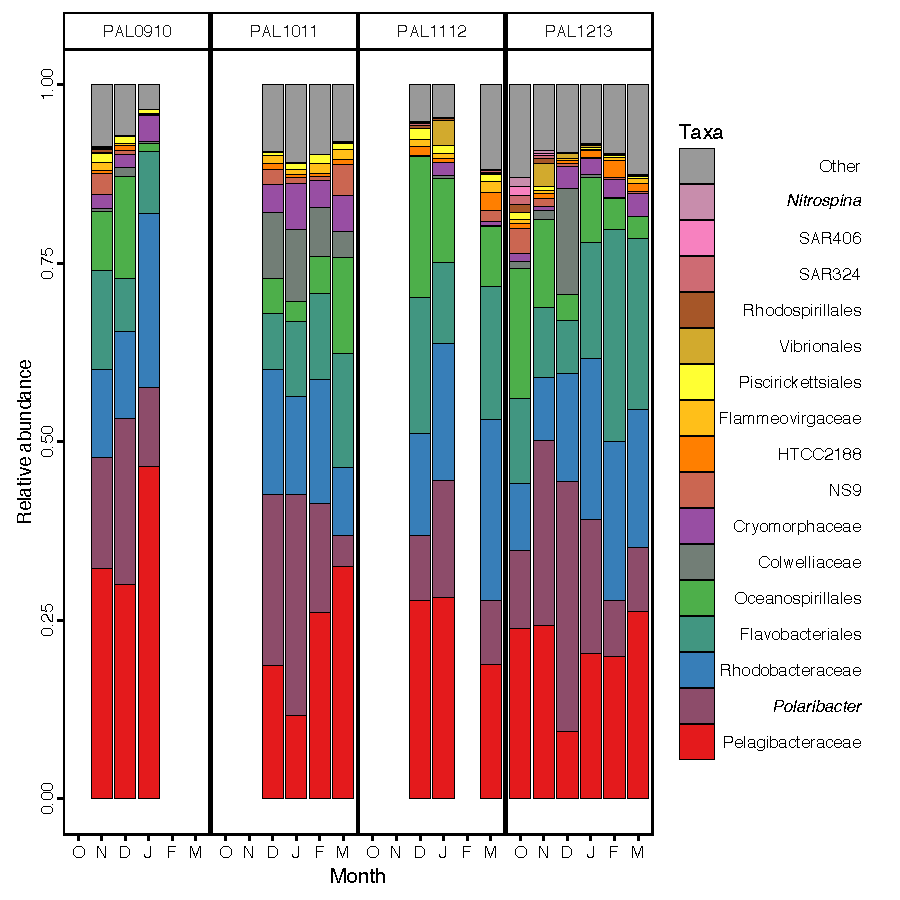
\includegraphics[width=0.8\textwidth]{Chapter_5_LTER/Figures/Figure_10_taxa_barplot}
\caption[Relative abundance of the 16 most common taxa.]{Relative abundance of the 16 most common taxa by mean relative abundance. Mean abundance is shown when more than one library is present for the month shown.} 
\label{fig:ch4:taxa} 
\end{figure}

In contrast to these broad trends, some individual taxa varied widely in abundance from year to year. For example, Colwelliaceae, although relatively rare in most of our samples, was fairly abundant throughout the PAL1011 season, and one Colwelliaceae OTU (810446) ``bloomed'' in December 2012, going from a {\textless}1\% relative abundance to a 30\% relative abundance in the course of one month (Figure \ref{fig:ch4:seasonal_otu} and \ref{fig:ch4:taxa}). Colwelliaceae responded very strongly to diatom-derived DOM during a series of mesocosm experiments (Chapter 4) and their abundance during PAL1011 may reflect the dominance of diatoms during that season and potentially again in December 2012 \citep{saba2014winter}. While PAL0910 was also a high chl \emph{a} year, our DNA time series did not encompass the late January 2010 phytoplankton bloom. During PAL1112, a low chl \emph{a} year, Colwelliaceae had very low relative abundance and we did not observe the midsummer shift between Pelagibacteraceae and \emph{Polaribacter} that occurred in other years.

A stepwise linear regression model based on serial day, daylength, and chl \emph{a} explained 43\% of the variation in richness ($p < 10^{-5}$). Bacterial production was eliminated during variable selection, despite its close association with bacterial community characteristics in our previous study \citep{luria2016seasonal}. Overall community similarities were correlated with a combination of abiotic (day length) and biotic (bacterial production and chl \emph{a}) factors (BIOENV, \emph{rho} = 0.38). BIOENV analysis results were stronger when seasons were considered individually (Table \ref{ch4:tab:bioenv}). For each season, either serial day or day length was an important factor, signaling ``seasonality''. Chl \emph{a} was an important variable in all but one season (PAL1011). Bacterial production was a significant variable in PAL0910, PAL1011, and PAL1213, while bacterial abundance was significant in PAL1112. Surprisingly, one or more macronutrients, which are seldom depleted in the WAP region, were significant for each season. Covariance with other factors may explain the inclusion of nutrients in final BIOENV models. Alternatively, while macronutrients are seldom depleted in the WAP region, they may become more limiting in years with positive chl \emph{a} anomalies \citep{Ducklow2007-ns,saba2014winter}. Overall, these relationships suggest that community structure is linked to both temporal factors with no interannual variability (e.g. day length and serial day) and biotic factors with a high degree of interannual variability (e.g. chl \emph{a} and bacterial production). 

\begin{table}[]
\centering
\caption[Results from BIOENV analysis, linking environmental variables to overall community similarity.]{Results from BIOENV analysis for individual LTER seasons and for all seasons pooled. Only environmental factors for which data was available for almost all dates were considered. These included: serial day, day length, bacterial abundance (BA), bacterial production (BP), phosphate, silicate, nitrate and nitrite, chlorophyll \emph{a} (chl \emph{a}), and phaeopigment.}
\label{ch4:tab:bioenv}
\small
\begin{tabular}{@{}lll@{}}
\toprule
Season     & Environmental factors                                    & BIOENV rho \\ \midrule
All pooled & Day length, BP, chl \emph{a}                             & 0.38       \\
PAL0910    & Serial day, BP, phosphate, silicate, chl \emph{a}, phaeopigment & 0.94       \\
PAL1011    & Serial day, day length, BP, phosphate                    & 0.81       \\
PAL1112    & Day length, BA, nitrate and nitrite, chl \emph{a}        & 0.58       \\
PAL1213    & Serial day, day length, BP, nitrate and nitrite, chl \emph{a}   & 0.66       \\ \bottomrule
\end{tabular}
\end{table}


To explore the relationship between community structure and biotic factors in greater depth, we tested the relationship between relative abundance for the top 100 individual OTUs (by mean relative abundance) and chl \emph{a} and bacterial production. Sixty OTUs correlated significantly with bacterial production, while just 10 correlated significantly with chl \emph{a}, the presumed underlying driver of bacterial production and community structure. A co-occurrence network analysis of individual OTUs associated with key predictive environmental parameters yielded similar results, with several OTUs from the Flavobacteria and Gammaproteobacteria clades associated with bacterial production while just one OTU, classified as \emph{Polaribacter}, was associated directly with chl \emph{a} (Pearson's \emph{r} {\textgreater} 0.5; Figure \ref{fig:ch4:network}). Pelagibacteraceae, which is more competitive under oligotrophic conditions, was negatively associated with bacterial production \citep{Tripp2013-zg}. 

\begin{figure}[ht!] 
\centering 
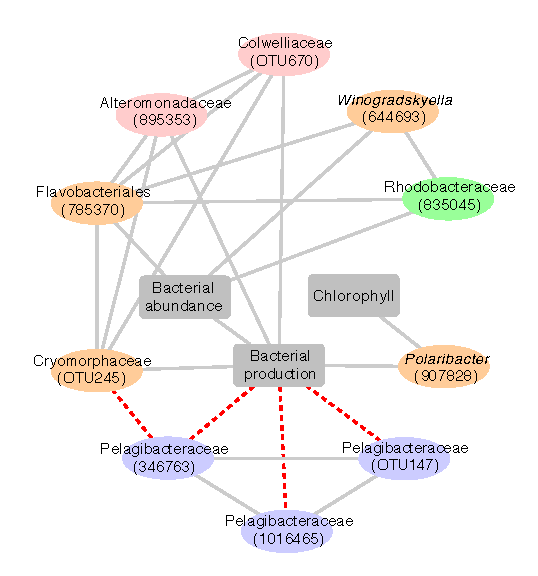
\includegraphics[width=0.8\textwidth]{Chapter_5_LTER/Figures/Figure_11_network_top100otus_minocc0_pearson5_subset_BA_BP_Chl}
\caption[Sub-networks of highly correlated OTUs built around chl a and bacterial production and abundance.]{Sub-networks of highly correlated OTUs built around chl \emph{a} and bacterial production and abundance ($r > 0.5$). Solid, grey lines represent positive correlations; dashed, red lines represent negative correlations. Closest taxonomic identification and reference number (in parentheses) are given for each OTU.} 
\label{fig:ch4:network} 
\end{figure}


While we hypothesized that changes in bacterial community structure would correspond strongly with phytoplankton dynamics, chl \emph{a} and primary production alone did not explain a large fraction of the observed variance in richness and community composition, nor were they significantly linked to many individual OTUs. \citet{kim2016decedal} report considerable interannual variability in the degree of chl \emph{a} control of bacterial production. Furthermore, varying temporal lags between Antarctic phytoplankton blooms and subsequent bacterial responses may confound efforts to model these relationships \citep{billen1991phytoplankton,ducklow2001seasonal,luria2016seasonal}. Such lags are attributed to the need for extracellular hydrolysis of high molecular weight phytoplankton-derived organic matter prior to bacterial uptake \citep{billen1991phytoplankton,ducklow2001seasonal,lancelot1991modelling,kirchman2001glucose}. Additionally, some DOM fractions may only become available through intermediate trophic processes (e.g. zooplankton sloppy feeding or excretion; \citealt{dsvse12}). Therefore, while chl \emph{a} may have been an underlying driver of bacterial community structure, intermediate modulating factors may have obscured its influence. 


We did not consider the influence of ``top-down'' controls, mortality due to bacteriophage induction and predation, which may increase as the season progresses. In the spring, when phytoplankton production and hence DOM availability are low, bacterial community structure is most likely governed by bottom-up controls \citep{bowman2016segmentation}. \citet{Brum2016-ig} report that most phage are in lysogenic phase in the spring and there may be insufficient grazers present to exert substantial top-down control at this point \citep{bowman2016segmentation}. Later in the year, phytoplankton growth may somewhat relieve DOM limitation, while viral abundance and predation may increase \citep{garzio2013microzooplankton,bird1999uncoupling}. As bacterivores and marine viruses disproportionately target rapidly growing cells, top-down controls have the potential to exert a significant control on midsummer bacterial community composition \citep{Fuhrman1993-zk,garzio2013microzooplankton}. 

\section{Conclusions}

Our time series of four LTER seasons encompassed considerable variability in winter/spring physical forcing of phytoplankton dynamics, and subsequently, in bacterial production and biomass, nutrient drawdown, and organic matter availability. Perhaps as a result, we did not observe robust seasonal patterns in OTU richness or strongly recurring annual successional trends for the overall community. Given the interannual variability in phytoplankton growth and a possible mid-season shift between bottom-up and top-down controls, it will be difficult to build robust models for bacterial community composition across multiple years in this dynamic system. However, seasonal trends emerged for individual taxa and OTUs, hinting at diverse ecological niches. The high degree of interannual variability that we observed suggests that multiple years of data encompassing complete SAM and ENSO cycles are needed to capture the range of bacterial community structures that occur in this system.
 

\chapter{Testing the impacts of cells, nutrients, and organic matter released into the water column during sea ice melt}\label{ch:seaice}


\chapterdisclaimer{This work was performed in collaboration with Hugh Ducklow, Linda Amaral-Zettler, and Jeremy Rich.\\
\\
Catherine Luria, Linda Amaral-Zettler, Hugh Ducklow, and Jeremy Rich designed and conducted the study. Catherine Luria analyzed data and wrote this chapter with guidance from Jeremy Rich. 
}


\section{Abstract}

Sea ice is a key driver of seasonal and interannual ecosystem variability in the coastal waters of the Antarctic Peninsula. When sea ice, which harbors a rich microbial community, melts in the spring, microbes, organic material, and nutrients are released into the water column. We conducted a series of four mesocosm experiments during two austral springs to test the impacts of these inputs on water column bacteria. We found little support for the ``seeding hypothesis,'' the conjecture that algae released during ice melt form the basis of the intense algae blooms often seen in the marginal ice zone (MIZ). However, we did observe increased bacterial abundance and production in response to both whole and filtered sea ice additions, suggesting that bacteria responded favorably to a dissolved component of sea ice meltwater. The variation in results across our experiments was notable and reflects the heterogeneous nature of our sea ice inocula. 

\section{Introduction}

Sea ice is an integral part of polar ecosystems \citep{thomas2003sea, wywabdlc13}. It covers 7\% of the Earth's surface on a seasonal basis and plays a vital role in physical regulation of the marine environment and hence the marine food web \citep{Maycut1985-ng}. The pelagic ecosystem west of the Antarctic Peninsula (WAP) has experienced a 40\% decline in sea ice extent over the past few decades, with an overall trend toward later advance and earlier retreat, shortening the annual duration of sea ice cover by over 80 days \citep{Stammerjohn2008-nj}. Because the annual retreat and advance of sea ice profoundly influence numerous WAP ecosystem processes, as well as many species, minor shifts in temperature, which cause declines in sea ice duration and extent, can dramatically impact ecosystem function \citep{Clarke2008-zv}. In addition, decreased sea ice extent and duration reduces surface albedo and ice thickness, allowing for greater ocean winter heat flux, positively feeding back into trends toward warmer air temperatures and sea ice decline \citep{Ducklow2007-ns}.

Sea ice advance begins in the austral autumn with the formation of frazil ice crystals which incorporate carbon- and microbe-rich summer surface waters \citep{Garrison1996-ro}. As sea ice continues to coalesce, numerous microhabitats form including brine channels that perforate the bottom surface of the ice. These brine channels provide a stable growth platform for winter phytoplankton, allowing phytoplankton to remain near the surface and maximize exposure to limited light. The sea ice microbial community accounts for 9-25\% of primary production in the ice-covered Southern Ocean \citep{Arrigo1997-bj}. Ice algae form the base of a winter food web, creating a nutrient and carbon enriched niche that supports ice-inhabiting bacteria and zooplankton \citep{Garrison1989-sn}. The algae also support a winter population of juvenile krill that live directly under the ice and in turn support a variety of marine birds and mammals \citep{Ducklow2007-ns}. As such, declines in sea ice have the potential to impact all levels of the marine food web. Previous studies have examined the effects of sea ice extent and duration on primary production \citep{Vernet2008-on}, krill \citep{Ross2000-mm}, and seabirds \citep{Croxall2002-ja}. Summer phytoplankton biomass, and hence bacterial production are lower in years with less winter sea ice \citep{saba2014winter, dsvse12}. However, we know little about the direct impacts of annual sea ice retreat on bacteria in the WAP water column.

 

When sea ice retreats in the austral spring, in addition to releasing freshwater that contributes to water column stratification, it releases phytoplankton, bacteria, organic matter and nutrients. The ``seeding hypothesis'' proposes that the release of phytoplankton seeds the water column, forming the basis of spring phytoplankton blooms. Although the seeding hypothesis has not been extensively tested, previous microcosm experiments suggest that seeding alters phytoplankton abundance and community composition \citep{Kuosa1992-vk,Giesenhagen1999-kq}. The effects of the release of dissolved organic matter (DOM) and seeding by either bacteria or phytoplankton on bacterial community composition remain uncharacterized. Because microbes form the basis of the marine food web and contribute disproportionately to ecosystem function, the impact of sea ice retreat on the microbial community could have far-reaching effects. Furthermore, without understanding these impacts, we cannot predict how rapid declines in sea ice extent and duration may alter the WAP ecosystem. We conducted a series of mesocosm experiments to test the impacts of both filtered and unfiltered sea ice additions on microbial community production, biomass, and abundance. We hypothesized that while the release of DOM would enhance bacterial production and abundance, sea ice algae and bacteria are uniquely adapted to the sea ice environment and would not flourish in the water column after sea ice retreat. 

\section{Methods}

Mesocosm experiments were conducted in October and November of 2012 and 2013 at Palmer Station, Antarctica. For sea ice ``treatments,'' brown sea ice (i.e. sea ice that visibly contained algae and/or organic matter) was collected in acid-washed buckets from the surface at either Station B or from the shoreline around Palmer Station. The sea ice was melted in \SI{0.2}{\micro\meter} filter-sterilized seawater (50\% w/v) in order to avoid cell lysis at \textasciitilde{}1$^{\circ}$C or at room temperature while ensuring that the water temperature never rose above 0$^{\circ}$C. After the ice was completely melted, half of the meltwater was passed through \SI{0.22}{\micro\meter} polyethersulfone (EMD Millipore, Billerica, MA) filters for the ``filtered ice'' treatment, while the remainder of the melted sea ice solution was left unfiltered for the ``whole ice'' treatment. The filtered seawater, filtered sea ice solution and unfiltered sea ice solution were sampled prior to initiating experiments for chlorophyll \emph{a} (chl \emph{a}) and phaeopigment, bacterial and phytoplankton abundance, and bacterial production as previously described \citep{Luria2014-dj}.

For each experiment, acid-washed 50 L polycarbonate carboys were filled directly from a seawater intake located at a depth of 6 m, 16 m from the shore. The intake was sampled prior to any filtering on station. The mesocosm experiments contained three groups: 1) control (no amendments), 2) 1\% v/v filtered sea ice solution addition (testing the effects of dissolved carbon and nutrient additions), and 3) 1\% v/v unfiltered sea ice solution (testing the effects of microbial seeding). For each group, triplicate 50-L carboys were incubated at ambient seawater temperatures for 10 days. A volume ratio of 1:100 represents the melting of a 10-cm-thick layer of sea ice in a 10-m deep mixed layer. We sampled the carboys on days 0, 2, 4, 6, 8 and 10 for phytoplankton abundance through flow cytometry (2012 only), chl \emph{a} (2013 only), and bacterial abundance and production (both 2012 and 2013). All sampling took place at incubation temperatures. Chl \emph{a} and bacterial production were measured as described in Chapter 3. Autofluorescent particles (i.e. phytoplankton) were counted live immediately after sampling on an Accuri C6 flow cytometer (BD Biosciences, San Jose, CA) equipped with a blue laser beam (50 mW, 488 nm). Particle size was determined by forward scatter versus side scatter comparison with fluorescent microspheres (Polysciences, Inc., Washington, PA) of varying size (\SIrange{0.5}{20}{\micro\meter}) as previously described \citep{garzio2013microzooplankton}. Bacteria were stained with SYBR\textsuperscript{\textregistered} Green I (Invitrogen, Carlsbad, CA) as described in Chapter 3 and were counted using an Accuri C6 flow cytometer (BD Biosciences, San Jose, CA) in 2012 and a Guava easyCyte flow cytometer (EMD Millipore, Billerica, MA) in 2013. 

\section{Results} 

In 2012, sea ice nanophytoplankton (\SIrange{2}{20}{\micro\meter}) were very abundant, ranging from $1.5 \text{ to } 7.0 \times 10^{6}$ cells ml$^{-1}$, about two orders of magnitude greater than abundance in the underlying water column (Figure \ref{fig:ch5:exp2012}). Likewise, in 2013, sea ice chl \emph{a} ranged from \SIrange{19}{29}{\micro\gram\per\liter}, as opposed to \SIrange{0.1}{0.2}{\micro\gram\per\liter} in the underlying water column. Bacterial abundance ranged from $1.1 \text{ to } 1.4 \times 10^{9}$ cells ml$^{-1}$ in 2012 and from $9.5 \times 10^{5}$ to $3.4 \times 10^{6}$ cells ml$^{-1}$ in 2013. In the water column, bacterial production averaged around \SI{6}{\pico\mole \per\liter \per\hour}. In sea ice, production was higher in November of both years, reaching almost \SI{700}{\pico\mole \per\liter \per\hour} in November 2013. Filtration reduced nanophytoplankton abundance by 100\% (2012), chl \emph{a} concentration by 99.9\% or more (2013), and bacterial abundance by 99\% or more. Bacterial production was reduced by more than 99\% during the 2012 experiments and by 92-94\% during the 2013 experiments.


\begin{figure}[htbp] 
\centering 
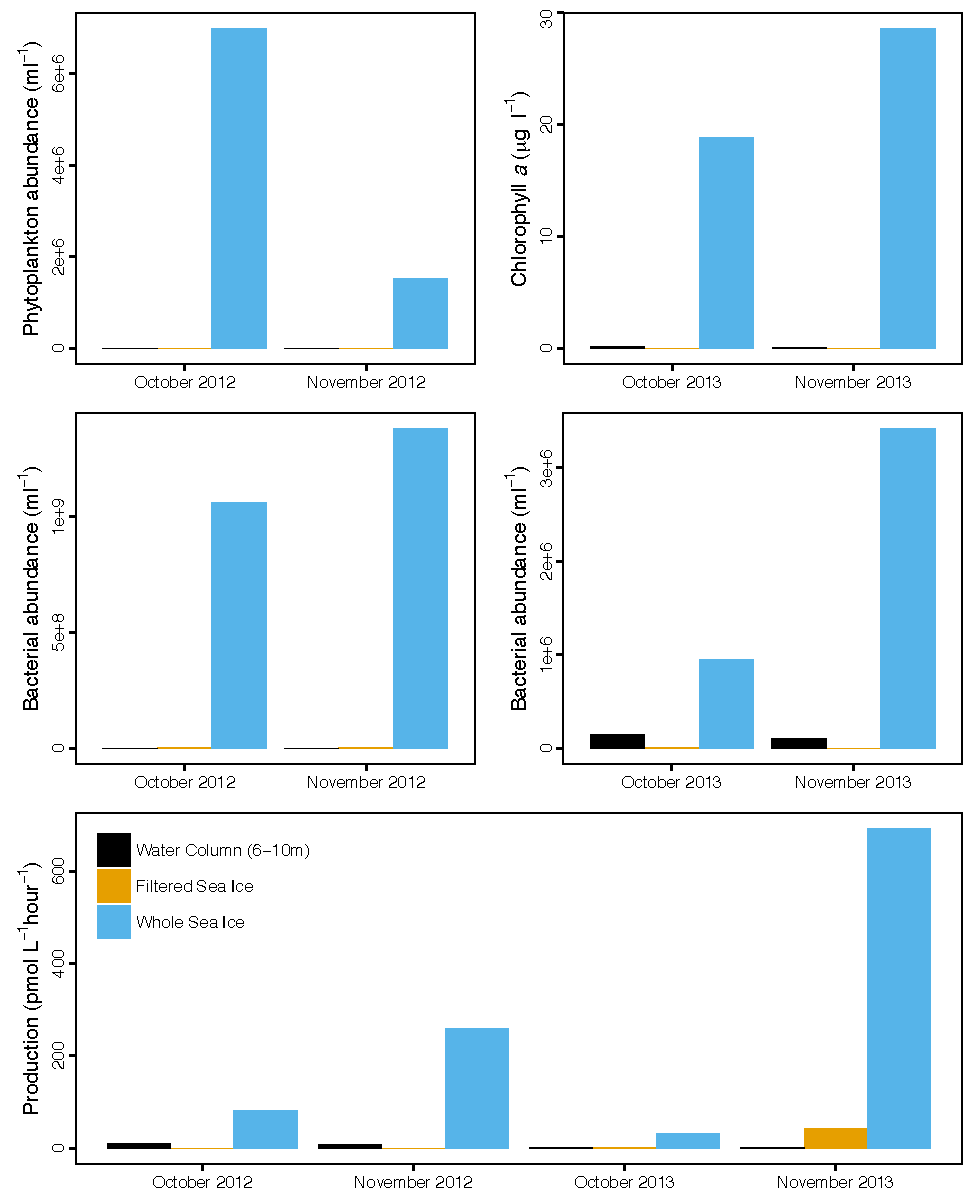
\includegraphics[width=0.9\textwidth]{Chapter_6_SeaIce/Figures/initial_values}
\caption{Initial phytoplankton abundance/biomass, bacterial abundance, and bacterial production values for filtered and unfiltered melted sea ice and the underlying water column.} 
\label{fig:ch5:exp2012} 
\end{figure}


During the October 2012 experiments, bacteria responded despite an apparent lack of phytoplankton growth under ice treatments (Figure \ref{fig:ch5:exp2013}). Nanophytoplankton abundance was actually greater in the control mesocosms for most of the experiment. Nonetheless, bacterial abundance and production increased substantially by Day 4 in both the filtered sea ice and whole sea ice mesocosms and remained higher through the rest of the incubation period. Likewise, in November 2012, nanophytoplankton abundance did not increase under sea ice treatments. Bacterial abundance was largely consistent across treatments. Bacterial production was greater on some days in the filtered ice mesocosms than in the control mesocosms. It was greater still in the whole sea ice mesocosms, and remained so throughout the experiment.

\begin{figure}[htbp] 
\centering 
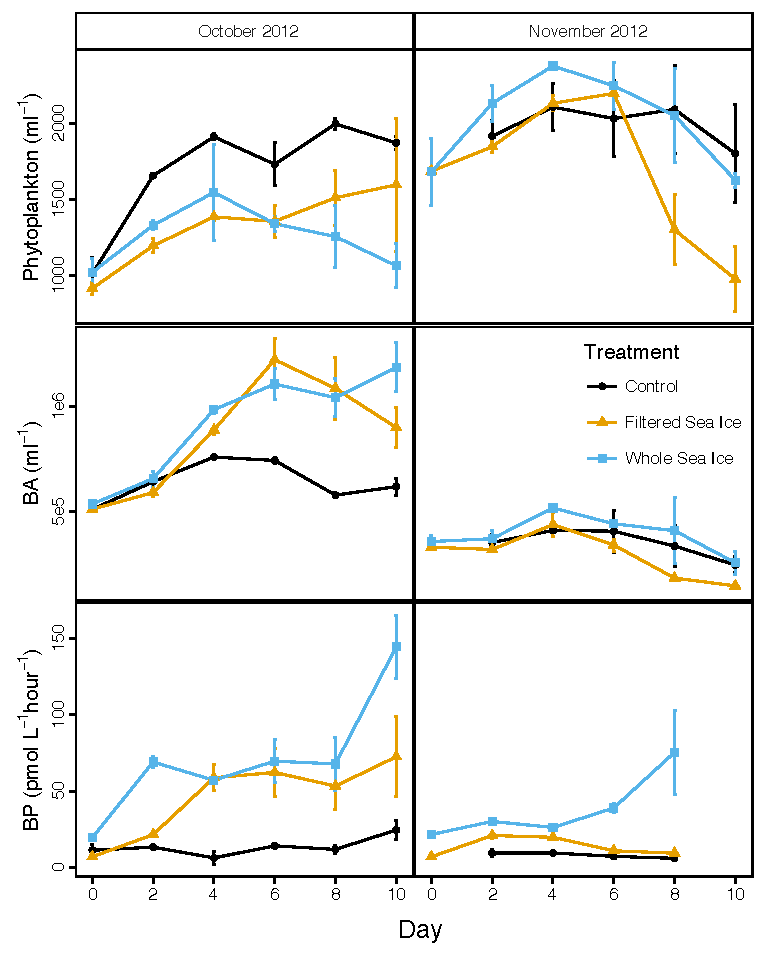
\includegraphics[width=0.9\textwidth]{Chapter_6_SeaIce/Figures/Experiments_2012}
\caption{Changes over a 10-day incubation period in phytoplankton abundance, bacterial abundance, and bacterial production in response to filtered and unfiltered sea ice additions, October and November 2012.} 
\label{fig:ch5:exp2013} 
\end{figure}

In contrast with the 2012 experiments, chl \emph{a} increased 2- to 7-fold under sea ice additions in both of the 2013 experiments (Figure \ref{fig:ch5:initial}). Chl \emph{a} was \textasciitilde{} \SI{0.2}{\micro\gram\per\liter} in the control and \textasciitilde{}\SI{0.8}{\micro\gram\per\liter} in the whole sea ice mesocosms at the initiation of the October experiment. It remained fairly stable in the control mesocosms, but reached \SI{1.3}{\micro\gram\per\liter} in the whole sea ice mesocosms by the end of the experiment. Chl \emph{a} started and ended lower in both the control and whole sea ice mesocosms in the November experiment compared to the October experiment, but levels in the whole sea ice mesocosms were still higher than in the control. Bacterial abundance was higher in both the filtered ice and whole ice mesocosms in October 2013. It was higher in the whole ice mesocosms only on days 2 and 4 in November 2013. Bacterial production was greatest in the filtered sea ice mesocosms on Day 2 in October 2013 and in the whole sea ice mesocosms in November 2013, but the trends were inconsistent and any changes were minor relative to those observed during the 2012 experiments.

\begin{figure}[htbp] 
\centering 
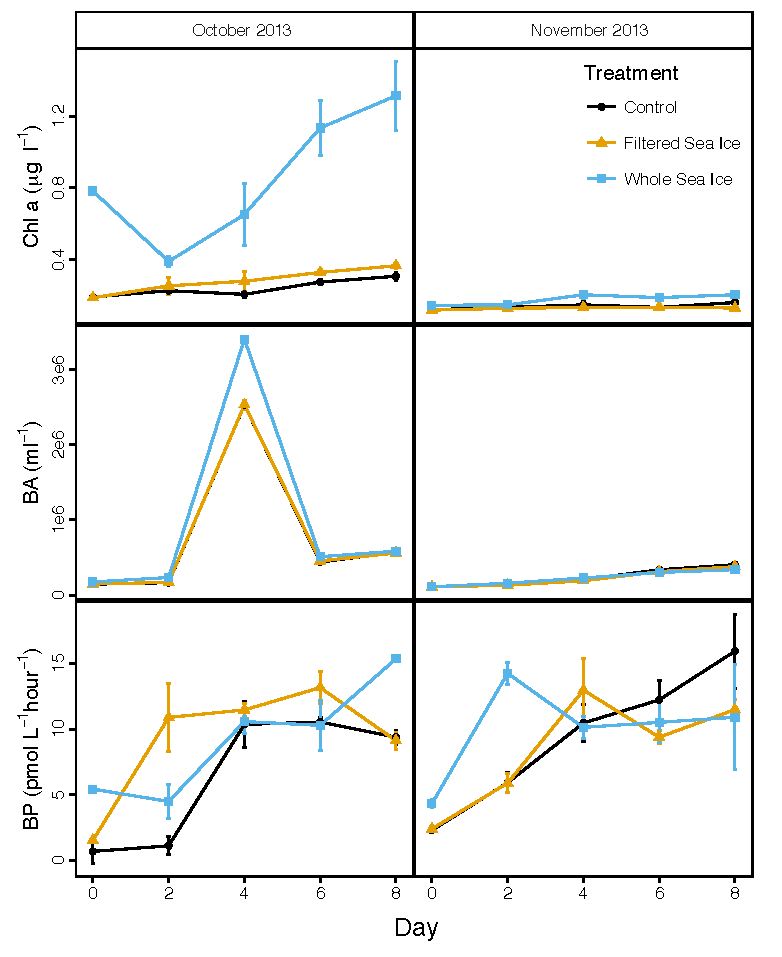
\includegraphics[width=0.9\textwidth]{Chapter_6_SeaIce/Figures/Experiments_2013}
\caption{Changes over a 8-day incubation period in phytoplankton biomass (chlorophyll \emph{a}), bacterial abundance, and bacterial production in response to filtered and unfiltered sea ice additions, October and November 2013.} 
\label{fig:ch5:initial} 
\end{figure}

\section{Discussion}

Phytoplankton blooms often track the receding ice edge in the spring \citep{Smith1985-lx,Smith1986-en} and summer phytoplankton biomass is greater in areas and in years with heavy winter sea ice \citep{Nicol2000-gd,saba2014winter}, giving rise to the ``seeding hypothesis'' in which inoculation of the water column by cells released from sea ice initiates phytoplankton blooms \citep{Garrison1989-sn,Garrison2007-ea}. Shared dominant species in sea ice and the neighboring MIZ provide support for this hypothesis \citep{Garrison1989-sn,Garrison1985-yg,Lannuzel2013-gk,Smith1986-en}. The increased chl \emph{a} in whole sea ice mesocosms in our 2013 experiments suggests that phytoplankton released from sea ice do in fact proliferate to an extent in the water column. However, the changes in phytoplankton biomass and abundance that we recorded were minor compared to changes during phytoplankton blooms in the environment. 

Sea ice contains abundant algal populations, with chl \emph{a} concentrations that can reach tens and hundreds of mg m$^{-3}$, and the presence of similar species in the MIZ suggests that sea ice is not necessarily populated by organisms that thrive exclusively in ice \citep{Garrison2007-ea}. However, numerous factors could influence the viability of potential seed populations within the ice. Meteorological and oceanographic conditions can affect the physical structure of sea ice \citep{Ackley1994-ld}, and subsequently algal access to nutrients and inorganic carbon \citep{Fritsen1994-zw,Gleitz1995-un}. Salinity varies greatly in sea ice; very high salinities can inhibit phytoplankton growth while very low salinity may lead to cell lysis \citep{Etheridge2005-vg,Garrison1985-yg}. The accumulation of low-salinity meltwater within or beneath the ice could lead to mass algal mortality during the melting process \citep{Lizotte2008-un}. In addition, a large fraction of ice algae have been shown to form aggregates, resulting in rapid sedimentation during melting \citep{Giesenhagen1999-kq,Riebesell1991-xy}. Perhaps, as a result, some studies have found that only small ice algae (<\SI{10}{\micro\meter}) persist in the water column \citep{Mathot1991-nv}. Together, these factors may alter the viability and species composition of the sea ice biota and the likelihood that this community will proliferate upon release into the water column. 

Whole sea ice additions actually reduced phytoplankton abundance in one of our experiments. \citet{Mathot1991-nv} and \citet{Lannuzel2013-gk} attribute reduced phytoplankton abundance during similar experiments to grazers. Heterotrophic species of chrysophytes, cryptophytes, and euglenophytes have been reported in sea ice \citep{Ikavalko1997-ak,Lizotte2008-un} and high grazing pressure was observed at the ice edge in the Weddell Sea \citep{Riebesell1991-xy}. Likewise, high virus counts were found in association with an ice algal bloom in the Arctic \citep{Maranger1994-uk}. Algal blooms within the ice itself, which can occur as light availability increases in the spring, increase the size of the potential seed community, but they may also increase the abundance of grazers just as sea ice is receding \citep{Leu2015-at}. 

Overall, our results suggest that the effects of seeding are quite minor. Previous studies based on mesocosm experiments provide conflicting evidence on this topic, reporting variously that that seeding effects are negligible \citep{Riebesell1991-xy}, patchy \citep{Kuosa1992-vk}, or substantial \citep{Giesenhagen1999-kq,Lannuzel2013-gk}. Therefore, we suspect that the physical changes wrought in the upper water column by sea ice retreat are of far greater significance to MIZ blooms. Sea ice melt freshens surface waters and subsequent shoaling of the upper mixed layer allows phytoplankton to persist and proliferate in the euphotic zone are far more significant than inconsistent seeding effects \citep{saba2014winter,Venables2013-me,Vernet2008-on}. The impact of water column stratification and potential interactions between stratification and seeding are impossible to test on the mesocosm scale.

While we found little evidence of phytoplankton seeding, we did observe bacterial responses to sea ice that were independent of sea ice-induced phytoplankton growth (c.f. \citealt{Lannuzel2013-gk} and \citealt{Giesenhagen1999-kq}). These responses were actually stronger in 2012 when we detected little, no, or even negative phytoplankton growth under sea ice treatments. Response levels were usually, but not always, similar between whole sea ice and filtered sea ice mesocosms, suggesting that bacteria reacted to an element found in the dissolved fraction of sea ice melt water (i.e. nutrients or organic matter). WAP bacterial growth is thought to be primarily limited by the availability of labile DOM \citep{dsvse12,Kirchman2009-sg}, which accounts for a large fraction of sea ice primary production \citep{Gosselin1997-qs}. Sea ice DOM might be especially abundant if mortality rates were high during melting. Ice DOM could be particularly important to bacteria as it enters the system in the spring before primary production in the water column partially relieves DOM limitation. While macronutrients are seldom limiting in the WAP region, micronutrients accumulated in sea ice may also stimulate growth \citep{Martin1990-ly}. For example, \citep{Loscher1997-ii} reported that iron concentrations were 2 to 100 times higher in sea ice than in the surrounding surface water. Therefore, sea ice melt water could have strong impacts on both bacterial and phytoplankton growth separate from the influences of seeding and water column stratification.

An insight from our results is the high degree of variability in our sea ice inocula and in subsequent impacts on bacterial growth. Phytoplankton biomass and bacterial production and abundance in the sea ice varied substantially between years and even between months within a single year. Bacteria responded more strongly to sea ice additions in 2012 than in 2013 and differences between the whole sea ice and filtered sea ice mesocosms were not consistent. A small body of papers report similar studies testing the the mechanisms controlling ice-edge plankton blooms, each tailored to address specific questions \citep{Giesenhagen1999-kq,Kuosa1992-vk,Lannuzel2013-gk,Riebesell1991-xy}. Significant variation in results between studies and between experiments within a single study is evident, and is sometimes attributed, as in our study, to differences in the original ice \citep{Kuosa1992-vk}. Experiments testing the effects of sea ice meltwater on marine microbes, as well as models of the large-scale impacts of sea ice melt on the marine environment must account for this high degree of heterogeneity in sea ice characteristics.

 

%----------------------------------------------------------------------------------------
%	THESIS CONTENT - APPENDICES
%----------------------------------------------------------------------------------------

\appendix % Cue to tell LaTeX that the following "chapters" are Appendices

% Include the appendices of the thesis as separate files from the Appendices folder
% Uncomment the lines as you write the Appendices

%\include{Appendices/AppendixA}
%\include{Appendices/AppendixB}
%\include{Appendices/AppendixC}

%----------------------------------------------------------------------------------------
%	BIBLIOGRAPHY
%----------------------------------------------------------------------------------------
\cleardoublepage
\phantomsection
\addcontentsline{toc}{chapter}{Bibliography}
\bibliography{BIB}

%----------------------------------------------------------------------------------------

\end{document}  
